\documentclass[12pt,letterpaper,final,oneside,openany,onecolumn,obeyspaces]{book} 												
\usepackage[lmargin=3.5cm,rmargin=2.5cm,tmargin=3.0cm,bmargin=3.0cm]{geometry}
%\usepackage[latin1]{inputenc}											%european 
\usepackage[table,xcdraw]{xcolor}
\usepackage[T1]{fontenc}
\usepackage{hyperref}
\hypersetup{
    colorlinks=false,
    pdftitle = {Seminario de Oscar y Thomas},
    bookmarks = true, 
    pdfpagemode = FullScreen, 
}
\usepackage[colorinlistoftodos]{todonotes}
\urlstyle{same}
\usepackage{longtable}
\usepackage{tabu}
%\usepackage{floatrow}
%\DeclareFloatFont{huge}{\huge}
%\floatsetup[table]{font=huge}
\usepackage[]{times}
\usepackage[spanish]{babel}													%español

%\usepackage{caption} 
%\captionsetup[table]{skip=10pt}
\usepackage[skip=0.5\baselineskip]{caption}

\newcommand\carlos[1]{\textcolor{red}{Nota de Carlos: #1}}
\newcommand\oscar[1]{\textcolor{blue}{Nota de Oscar: #1}}
\newcommand\thomas[1]{\textcolor{green}{Nota de Thomas: #1}}

\usepackage{amsmath}	%math package
\usepackage{graphicx}
\usepackage{multicol}
\usepackage{url}
\usepackage[utf8]{inputenc}
\usepackage{amssymb}
\usepackage{array}
%\usepackage{algorithm_spa}
\usepackage{algpseudocode}
\usepackage[footnotesize]{subfigure}
\usepackage{makeidx}
\usepackage{color}

\makeindex
\renewcommand{\baselinestretch}{1}
\renewcommand{\contentsname}{Índice General}%{Tabla de Contenidos}
\renewcommand{\listfigurename}{Lista de Figuras}
\renewcommand{\listtablename}{\'Indice de Tablas}
\renewcommand{\chaptername}{Capítulo}
\renewcommand{\bibname}{Bibliografía}
\renewcommand\floatpagefraction{.9}
\renewcommand\topfraction{.9}
\renewcommand\bottomfraction{.9}
\renewcommand\textfraction{.1}
\addto\captionsspanish{%
  \renewcommand{\tablename}%
    {Tabla}%
}

\setcounter{totalnumber}{50}
\setcounter{topnumber}{50}
\setcounter{bottomnumber}{50}

% Different font in captions
\newcommand{\captionfonts}{\small}
\newcommand{\tabitem}{\textbullet~~}
\makeatletter  % Allow the use of @ in command names
\long\def\@makecaption#1#2{%
  \vskip\abovecaptionskip
  \sbox\@tempboxa{{\captionfonts #1: #2}}%
  \ifdim \wd\@tempboxa >\hsize
    {\captionfonts #1: #2\par}
  \else
    \hbox to\hsize{\hfil\box\@tempboxa\hfil}%
  \fi
  \vskip\belowcaptionskip}
\makeatother   % Cancel the effect of \makeatletter

%Inicio de documento
\begin{document}
\hyphenation{pa-la-bra}

\renewcommand{\contentsname}{Tabla de Contenidos}
\renewcommand{\listfigurename}{Lista de Figuras}
\renewcommand{\listtablename}{Lista de Tablas}
	\frontmatter
		\label{ch:portada}
\thispagestyle{empty}

%\vspace{-2.0cm}
	\begin{figure}[t]
						\centering
							\includegraphics[height=0.15\textwidth]{./images/logoUCV.jpg}
	\end{figure}
					\begin{center}
						Universidad Central de Venezuela\\
						Facultad de Ciencias\\
						Escuela de Computaci\'on\\
					\end{center}
					
					\vspace{2.2cm}
					\begin{center}
						\huge{\textbf{Diseño e implementación de tests para simular fallos en entornos de cómputo híbrido}}
					\end{center}

					\vspace{2.2cm}
					\begin{center}
						Trabajo Especial de Grado \\
						presentado ante la Ilustre\\
						Universidad Central de Venezuela\\
						Por los Bachilleres\\
						Oscar Gerdel Sirit\\
						Thomas Alfonso\\
						para optar el título de \\
						Licenciado en Computaci\'on
					\end{center}
					
					\begin{center}
						Tutores:\\
						Prof. Robinson Rivas\\
						Dr. Carlos D. Camacho Gonz\'alez
					\end{center}
					
					\vspace{1.0cm}
					\begin{center}
						Caracas, Abril de 2021
					\end{center}
						
					
%\newpage
		\chapter{Agradecimientos}

En primer lugar queremos agradecer a nuestros tutores el Prof. Robinson Rivas y al Dr. Carlos Camacho quienes nos brindaron tutoría, apoyo y tiempo, además de retar nuestras habilidades a lo largo de todas las etapas de este proyecto para lograr los objetivos que deseábamos; sin lugar a duda son un gran ejemplo de docencia.\\

También queremos agradecer a la Universidad Central de Venezuela y sus profesores, que representaron una fuente de inspiración y aprendizaje, cuya calidad docente y humana es innegable, siendo nuestra guía para vencer la sombra.\\

Por último, queremos agradecer a todos nuestros compañeros y familia, por apoyarnos aún cuando nuestros ánimos decaían. En especial, queremos hacer mención de nuestros padres, que siempre estuvieron ahí para darnos palabras de apoyo y un abrazo reconfortante para renovar energías.\\

Muchas gracias a todos.\\

	%opcional
		%\input{dedicatoria}		%opcional
		\chapter*{Resumen}



\noindent \textbf{Titulo:}\\ 
Diseño e implementación de tests para simular fallos en entornos de cómputo híbrido \\
\noindent \textbf{Autores:}\\
Thomas Alfonso, Oscar Gerdel \\ 
\noindent \textbf{Tutores:}\\
Prof. Robinson Rivas, Dr. Carlos D. Camacho González\\

En la actualidad, la computación en la nube exhibe un gran auge. La migración de sistemas monolíticos a arquitecturas basadas en microservicios, obliga a los desarrolladores a proporcionar soluciones cuando surgen problemas en un sistema por fallas en el entorno de computo híbrido. Por lo tanto ha surgido la
 tendencia de inyectar fallas a los sistemas y estudiar su comportamiento. Por lo expuesto previamente, en el presente trabajo de investigación se realizó un amplio estudio sobre nube híbrida, inyección de fallas, ingeniería del caos y algunas herramientas de configuración en computación, destacándose en Kubernetes y Ansible, 
%  que se usaron para establecer un entorno de pruebas, 
 que permitió diseñar e implementar fallas automatizadas y controladas que afectan la latencia, el CPU, el Disco y la memoria RAM de pods en un único nodo de Kubernetes, y así poder analizar el comportamiento del sistema ante fallas, obteniendo como resultado un degrado en la eficiencia del pod pero no hubo interrupción del servicio.\\    

% Esbozo sucinto del contenido del TEG, presentando objetivos, resultados y conclusiones (m\'aximo media p\'agina). \\

\noindent \textbf{Palabras Claves:}\\ 
Inyección de fallas, Kubernetes, Computo híbrido,
		\tableofcontents %indice
		\listoffigures	%opcional
		\listoftables		%opcional
		\chapter{Introducci\'on}

\par El impacto de la globalización en todas nuestras tareas, nos ha llevado a cambiar la manera  de realizarlas. El mundo de las comunicaciones y la informática no escapa a ello, las transformaciones requeridas por el constante avance tecnológico exige a los proveedores de servicios de computación a través de Internet, ofrecer a los usuarios sistemas confiables que reporten amplios beneficios. \\
 
\par En la actualidad, la computación en la nube exhibe un gran auge. La migración de sistemas monolíticos a arquitecturas basadas en microservicios, obliga a los desarrolladores a proporcionar soluciones cuando surgen problemas en un sistema por fallas en el entorno de computo híbrido. Es por ello, que la aplicación de técnicas para la detección de fallas que permitan el monitoreo del sistema, evitarían pérdidas de servicio y de dinero tanto para los proveedores de servicios como para los usuarios y empresas contratantes.\\


\par El presente trabajo de investigación, plantea la problemática del comportamiento del sistema en un entorno de nube híbrida ante una falla eventual. El problema se propone tratar desarrollando una herramienta para insertar fallas en el sistema y evaluar su respuesta.\\ %,con el fin de generar útiles reportes de falla-impacto.\\

\par Las grandes empresas como Netflix, Uber y WeChat aplican actualmente la ingeniería del caos en sus servicios. Esta nueva disciplina, basada en la inyección de fallas, agrega pruebas de tolerancia a fallas y confiabilidad del sistema, en un ambiente de producción con datos y eventos reales.\\

\par El presente estudio está conformado por cuatro (4) capítulos. El Capítulo 1 presenta el planteamiento del problema, la justificación y las limitaciones para la realización del mismo. En el Capítulo 2 se presenta el marco teórico continuativo de todos aquellos conceptos y procesos asociados con la nube hibrída y la inyección de fallas, además de una comparación de variantes de aplicación de esta técnica y la revisión de algunas herramientas de configuración en computación. El Capítulo 3 contiene el marco procedimental y en el se explica las metodologías más utilizadas en el desarrollo de software. En el Capítulo 4 se presenta la propuesta de Trabajo Especial de Grado, se plantea el objetivo general, los objetivos específico, la metodología propuesta, el alcance de la investigación, la arquitectura propuesta, las actividades realizadas para la implementación y a su vez los experimentos con sus resultados.


	\mainmatter
		\chapter{Planteamiento del Problema}
\par El auge de la computación en la nube ha propiciado, una nueva forma de interacción con los datos en el campo de la Tecnología de la Información (TI), que mejora la colaboración entre los desarrolladores, así como el escalado y la disponibilidad del sistema, al mismo tiempo que reduce de manera efectiva el costo y el mantenimiento de algún  proyecto que requiera de cómputos distribuidos. El uso extensivo de los servicios basados en la nube para alojar aplicaciones empresariales, conduce a problemas de disponibilidad y confiabilidad del servicio tanto para los proveedores  como para los usuarios de los mismos \cite{PLAN01,PLAN03}. Estos problemas son intrínsecos a la computación en la nube debido a su naturaleza altamente distribuida, la heterogeneidad de los recursos y la escala masiva de operación. En consecuencia, pueden ocurrir varios tipos de problemas en el entorno de la nube que conducen a fallas y degradación del rendimiento.\\

\par Los principales tipos de fallas \cite{PLAN04,PLAN05} son:
\begin{itemize}
    \item Falla de red : Una causa predominante de fallas en la computación en la nube son las de red, ya que el acceso a los recursos de computación en la nube se realiza a través de ella, verbigracia  Internet.  Puede ocurrir debido a particiones, pérdida o corrupción de paquetes, congestión, falla del nodo o enlace de destino, entre otras.
    \item Fallos físicos: Son aquellos que se producen principalmente en recursos de hardware, como fallos en CPU, memoria, almacenamiento, fallo de alimentación, etc.
    \item Fallos del proceso: Pueden producirse fallos en los procesos debido a la escasez de recursos, errores en el software, capacidades de procesamiento incompetentes, etc.
    \item Fallo de caducidad del servicio: Este tipo de falla ocurre, cuando el tiempo de servicio de un recurso caduca mientras una aplicación que lo arrendó lo está usando.
\end{itemize}

\par De modo que,  las fallas antes descritas conducen a problemas o al apagado de un sistema. Sin embargo,  la computación distribuida y por consiguiente, la computación en la nube se caracterizan por la noción de fallas parciales que pudiesen ocurrir en cualquier nodo constituyente, proceso o componente de red y en consecuencia, a una degradación del rendimiento en lugar de una falla completa. Aunque esto da como resultado sistemas robustos y confiables, las fallas deben manejarse de manera efectiva mediante mecanismos adecuados de tolerancia a fallas para la computación de alto rendimiento que permitan que el sistema atienda la solicitud, incluso si algunos de los componentes no funcionan correctamente. \cite{PLAN01,PLAN06}.\\

\par  El despliegue de sistemas de monitoreo de tolerancia de fallas en arquitectura de nubes, especifícamente las híbridas es un tema de actualidad \cite{PLAN02}, propiciado por la amplia aceptación e introducción durante la última década de aplicaciones con este tipo de infraestructura en la nube en base a contenedores, que posibilitan ventajas en portabilidad, escalabilidad y eficiencia.\\
 
\par Es por ello, que con la amplia utilización de nube híbrida llega la necesidad de monitorear y testear dichas aplicaciones, no solamente las tecnologías de desarrollo que utilizan, sino también las redes y el hardware que permiten el funcionamiento del sistema. Los softwares alojados en contenedores usan comúnmente un enfoque de microservicios, lo que si bien propicia mayor eficiencia también exige un conocimiento más detallado y especifico de la arquitectura utilizada.\\
\par Así, para monitorear estos sistemas es común utilizar una gran cantidad de comandos específicos, requiriendo mayor conocimiento y consumo de tiempo para poder comprender y estructurar el sistema de monitoreo.
%%%%%%%%%%%%%%%%%%%%%%
\section{Justificación y Limitaciones}

\par En la actualidad, la computación en la nube se ha convertido en un gran mercado y es por ello, que los proveedores se han apresurado a promocionar los éxitos en la nube resaltando los enormes beneficios que han obtenido determinadas compañías, al adoptar la computación en la nube.\\

\par Sin embargo, no todos los despliegues en la nube son exitosos.  Algunas  fallas, como cortes e incidentes de seguridad han afectado a los entornos de nube tanto públicos como privados, impactando de forma negativa a los proveedores de servicios en la nube puesto que aseguran, proporcionar servicios altamente disponibles y rentables pero estos no siempre funcionan así.\\
\par En efecto, la computación en la nube está sujeta a fallas que enfatizan la necesidad de abordar la disponibilidad del usuario, la cual está referida a la capacidad del sistema para operar continuamente.\\

\par  Es oportuno mencionar, algunos casos bastante emblemáticos que pueden ilustrar situaciones como las antes descritas como son por ejemplo, lo acontecido el 1 de octubre de 2013, cuando el gobierno federal de EE. UU. lanzó HealthCare.gov, un nuevo sitio web destinado a permitir que las personas se inscriban para comprar un seguro de salud en virtud de la Ley de Protección al Paciente y Cuidado de Salud Asequible\cite{PLAN09}. Casi de inmediato, los usuarios comenzaron a experimentar dificultades y algunos informes indicaron que menos del 1 por ciento de las personas que querían registrarse en línea pudieron hacerlo. Aunado a esto, no solo el proyecto superó el presupuesto acumulando más de US\$1.7 mil millones en costos por encima de un presupuesto original de solo US\$ 93.7 millones, sino que también, muchos observadores señalaron entonces, que el gobierno podría haber evitado estos problemas si hubiera utilizado un conocido proveedor de computación en la nube, en lugar de tratar de construir la infraestructura sobre equipos heredados. Más aun, criticaron a los desarrolladores por pruebas inadecuadas y falta de supervisión y responsabilidad \cite{PLAN09}.\\

\par Otros casos significativos, fueron  los  que experimentaron Amazon S3 y Google Gmail en el 2008, cuando la primera tuvo dos interrupciones de servicios: dos (2) horas en el mes de febrero y ocho (8) horas en el mes de agosto, mientras la segunda sufrió dos interrupciones de dos (2) horas cada una  en el mes de agosto \cite{PLAN11}.\\

\par Cabe destacar también, cuando en el 2009 en Salesforce.com, una de las empresas líderes que ofrecen software en la nube, sufrió una interrupción del servicio debido a una falla del dispositivo de red causada por errores de asignación de memoria, que impidió el procesamiento de datos en Europa, Japón y América del Norte durante 38 minutos. Unos pocos meses después, ocurrió una incidencia similar, que afectó a Europa y América del Norte durante algunas horas y causó que los clientes cuestionaran fuertemente la disponibilidad de servicios en la nube \cite{PLAN08,PLAN10}. A ello se suma, que en el año 2016 se produjo una gran interrupción que provocó inestabilidad en el servicio, durante dos (2) días hábiles.\\

\par Ahora bien, algunas de las principales soluciones implementadas por  empresas de alto perfil como AWS y las antes mencionadas  Google AppEngine y Salesforce, a las  fallas ocurridas fueron: alta calidad y mantenimiento regular del componente de hardware, redundancia de datos, detección de fallas, respaldo, autoescalado, uso de BigTable para almacenamiento de datos, escalabilidad de infraestructura, alto nivel de abstracción, plataforma de bloqueo y arquitectura redundante.\\

\par Por consiguiente, las fallas pueden ocurrir tanto en la nube como en un entorno tradicional de tecnología de la información (TI). Por lo antes expuesto esta investigación se justifica, porque aun cuando la nube permanecerá sujeta a fallas y no se puede garantizar una infinita disponibilidad, se puede aumentar y mejorar, evitando fallas comunes del sistema mediante el despliegue de diferentes soluciones  y técnicas \cite{PLAN09}.\\

\par Asimismo, es importante abordar esta investigación ya que permite comprobar la idoneidad  de la herramienta de inyección de fallas para la detección  y la tolerancia a ellas, no solo en un entorno tradicional de TI \cite{LIB01}, sino también su utilización en uno de computo  híbrido como la nube \cite{PLAN08,PLAN12} . En efecto, la mayoría de las aplicaciones modernas  se desarrollan en plataformas ubicuas, es decir, nubes y se diseñan como microservicios. Tal es el caso de empresas como Uber, WeChat, y Netflix, entre otras que  utilizan este tipo de plataformas y hacen uso extensivo de ellas . Es por ello, que al usar inyección de fallas se puede determinar si el sistema se comporta como es debido \cite{LIB12}.\\

\par  Además, es relevante porque permitirá  prevenir fallos en las plataformas al determinar de manera fiable, el comportamiento del sistema ante una eventual falla  y de esta manera, evitar pérdidas de servicio que se traducen en costos expresados en dinero, tanto para los proveedores de servicios en la nube como para las empresas contratantes de los mismos.\\

\par Por lo que respecta a las limitaciones, los autores expresan que en el curso de su investigación no han encontrado obstáculos para su realización, aun cuando  no se encontró mucha literatura especializada y referencias a la utilización de la herramienta de inyección de fallas en nube híbrida, lo que refuerza la novedad de la investigación.\\


%%%%%%%%%%%%%%%



		\chapter{Marco Teórico}

%%%%%%%%%%%%%%%
\par Los conceptos teóricos son fundamentales porque son las bases que sustentan una investigación. Es por ello, que conocer  los mismos permitirá una mayor comprensión global del trabajo investigativo.\\

\par Por consiguiente, en este capítulo se describen los conceptos y procesos asociados con el tema de estudio, su vinculación, comparación de variantes de aplicación  y revisión de algunas herramientas de configuración en computación.  


\section{Nube Híbrida}

\par La computación en la nube se refiere a la tecnología que permite mover y/o alojar servicios, cómputo o datos, fuera del sitio a una instalación o proveedor centralizado, externo o transparente, de ubicación centralizada, para obtener un costo y una ventaja comercia al hacer que los datos estén disponibles más fácilmente. La computación en la nube se puede desplegar de la siguiente manera \cite{LIB21}:\\

\begin{itemize}
    \item Nube privada: la infraestructura de la nube es exclusiva de una organización. Puede ser administrada por la organización o por un tercero y puede existir dentro o fuera de su establecimiento.
    \item Nube pública: la infraestructura de la nube se pone a disposición del público o de un grupo industrial y por lo general es propiedad de una organización que vende servicios en la nube.
    \item Nube híbrida: la infraestructura de la nube es una composición de dos o más nubes que siguen siendo entidades únicas pero están unidas.
\end{itemize}

\par Un entorno de nube híbrida, comprende un recurso de procesamiento para desplegar y administrar una aplicación en varios entornos de nube. En la figura \ref{fig:cloud01} se muestran los tipos de servicios mas comunes para la computación en la nube.\\
\begin{figure}[htpb!]
	\centering
	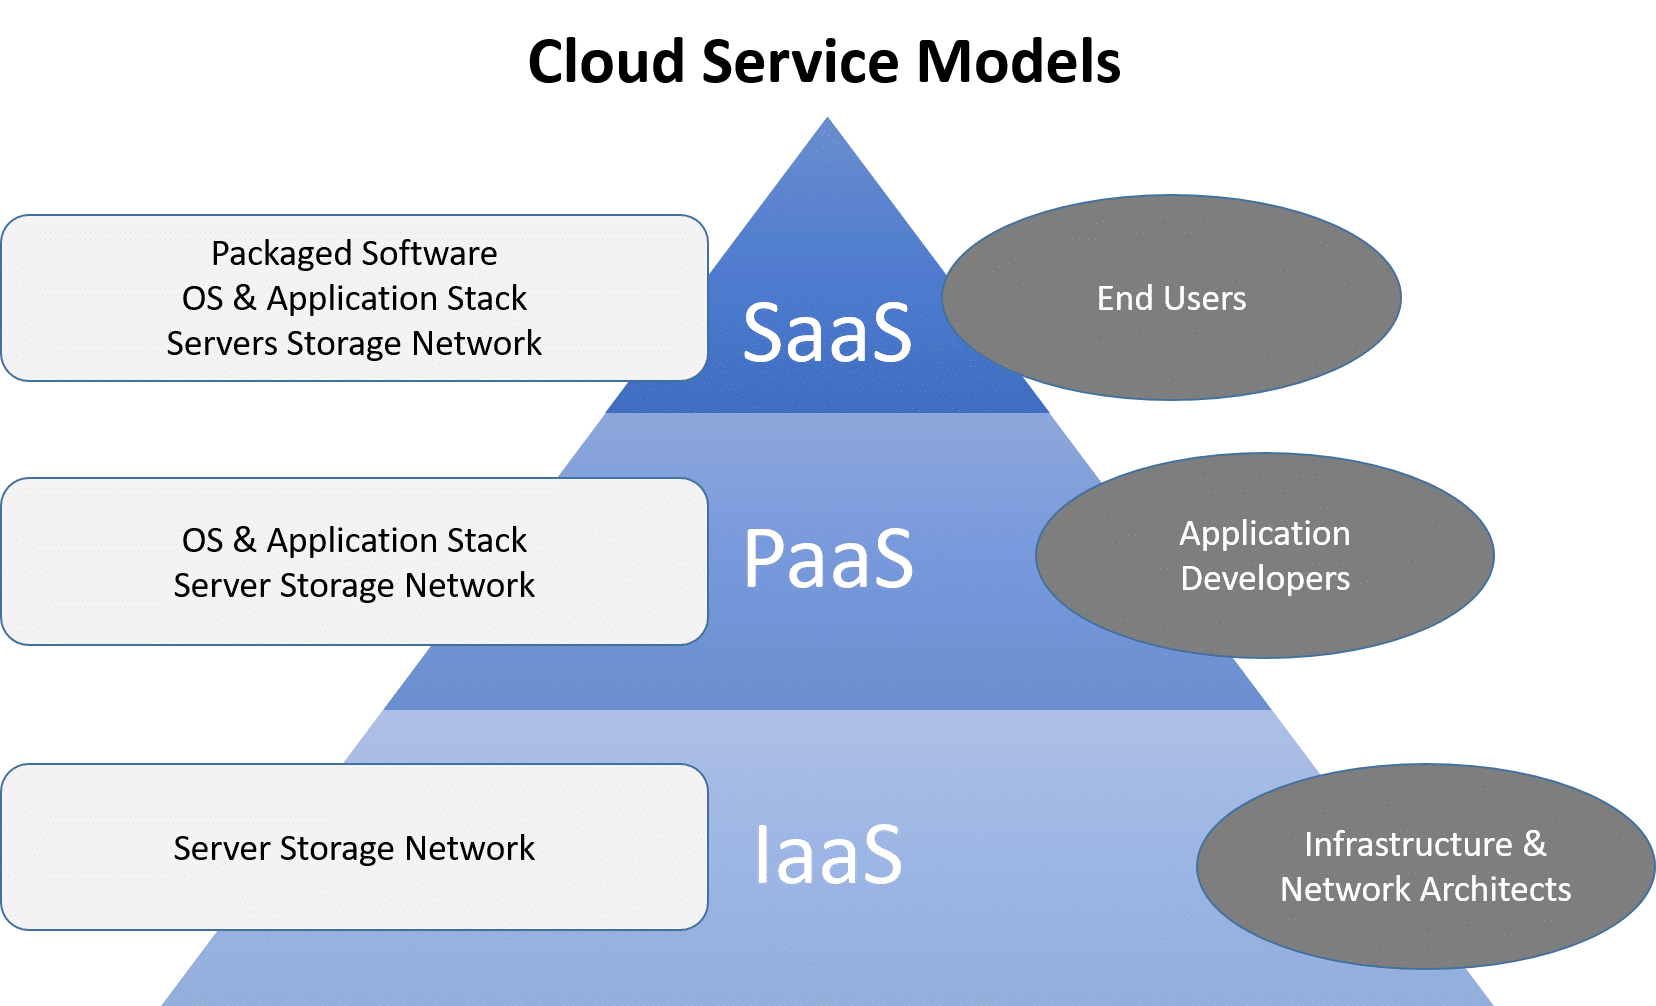
\includegraphics[width=0.8\columnwidth]{images/cloud01.png}
	\caption{Tipos de Servicios de la Nube.}
	\label{fig:cloud01}
\end{figure}

\par Hoy en día es común el despliegue de  Nube híbrida entre las empresas, ya que ella ofrece flexibilidad para combinar entre nubes públicas y privadas, dependiendo de sus necesidades de seguridad y accesibilidad de los datos, ubicación de los datos almacenados y otros servicios asociados a estos despliegues \cite{LIB21}.\\

\par La nube híbrida se define como una composición de dos o más infraestructuras de nubes (privadas, comunitarias o públicas), que siguen siendo entidades únicas pero están unidas por tecnología estandarizada o patentada que permite la portabilidad de datos y aplicaciones (combinación de nubes para el equilibrio de carga entre estas, Ver Figura \ref{fig:cloud02}) \cite{LIB21}.\\

\begin{figure}[htpb!]
	\centering
	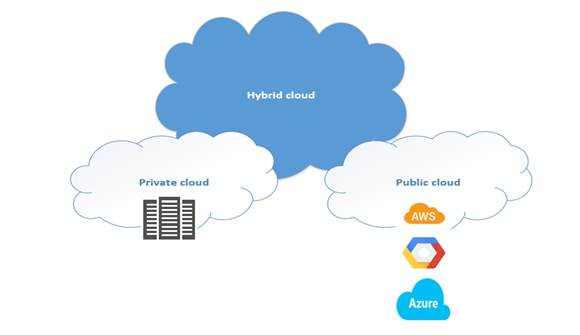
\includegraphics[width=0.8\columnwidth]{images/cloud02.png}
	\caption{Representación de la Nube Híbrida.}
	\label{fig:cloud02}
\end{figure}

\par La nube híbrida ofrece un enfoque simple donde las nubes unidas, se combinan como una plataforma que brinda el máximo valor y efectividad de cada componente de una carga de trabajo. En el paradigma híbrido, el sistema vive donde tiene más sentido: in situ o alojado, virtualizado o en la nube.\\

\par En la actualidad, el paradigma de la nube híbrida es utilizado para dar soporte a arquitecturas basadas en microservicios, las cuales hacen uso de contenedores, tal es el caso de Dockers, así como herramientas para la orquestación como Kubernetes y Dockers Swarm, de dicha virtualización ligera.\\


\subsection{Microservicios}

\par Cuando el uso de una aplicación crece, su propietario la escala para manejar el aumento del tráfico. Para compensar la rigidez de la escala vertical, se esta promoviendo la arquitectura de microservicio, que ve las aplicaciones desacopladas en unidades lógicas y divididas en microservicios \cite{LIB08}.\\

\par En la arquitectura basada en microservicios, la aplicación es una colección de servicios web, cada uno con un único propósito. Cada microservicio se desarrolla, despliega y administra de manera independiente, sus nuevas características y actualizaciones se agregan continuamente.\\
\par Por otra parte, las aplicaciones de microservicio suelen ser políglotas: los desarrolladores escriben microservicios individuales en el lenguaje de programación de su elección y la comunicación entre servicios se realiza mediante llamadas API remotas\cite{LIB08}. Los servicios se empaquetan en imágenes de contenedores de Docker y se despliegan haciendo uso de un orquestador como Kubernetes o Docker Swarm, que maneja el alojamiento, la escala y la supervisión.\\

\par Las aplicaciones de Internet a gran escala como Netflix, Facebook, la tienda de Amazon y otras, han demostrado que para lograr escalabilidad, robustez y agilidad es necesario dividir una aplicación web monolítica en una colección de servicios web o microservicios especializados \cite{LIB08}.\\

\begin{figure}[htpb!]
	\centering
	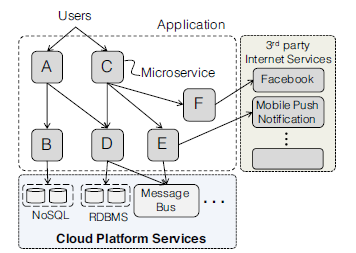
\includegraphics[width=0.8\columnwidth]{images/mserv01.png}
	\caption{Arquitectura típica de una aplicación basada en micro servicios \cite{LIB08}}
	\label{fig:mserv01}
\end{figure}

\par En la Figura \ref{fig:mserv01} se muestra una aplicación basada en microservicios. La aplicación aprovecha los servicios proporcionados por la plataforma de alojamiento en la nube (por ejemplo, bases de datos administradas, análisis de datos) y se integra con servicios de Internet, como redes sociales, geolocalización, etc.

\subsection{Kubernetes}
\par En los centros de datos modernos, los contenedores han cambiado la forma en que las aplicaciones se empaquetan, distribuyen y despliegan. Los contenedores proporcionan la abstracción perfecta para aplicaciones complejas en forma de una imagen, que agrupa las aplicaciones junto con sus dependencias en un ente único fácil de distribuir y ejecutar bajo un motor en tiempo de ejecución de contenedor como \textit{Docker}.\\
\par Los contenedores ofrecen una alternativa más ligera y ágil a las máquinas virtuales para el aislamiento entre aplicaciones y elevan su potencial en términos de rendimiento, utilización de recursos y portabilidad entre plataformas. La facilidad para construir y ejecutar contenedores ha propiciado el despliegue de aplicaciones de muy alta densidad y con esto, la necesidad de herramientas más robustas para la administración de contenedores \cite{BOOK04}.\\
\par Para desplegar ciertas aplicaciones, algunos contenedores deben desplegarse y administrarse. Para optimizar este proceso, el despliegue de estos contenedores se puede automatizar. Esto es especialmente útil si se utiliza un alto número de hosts. 
como Kubernetes, Mesos y Docker swarm, entre otras. Kubernetes es una de las herramientas de orquestación más ricas en características, con mayor documentación y se usa ampliamente en la actualidad \cite{BOOK02}.

\subsubsection{Funciones de Kubernetes}
\begin{itemize}
    \item Preparar y equipar hosts.
    \item Instanciar un conjunto de elementos deseados.
    \item Mantener pods fallidos, por ejemplo, mediante la reprogramación de los mismos.
    \item Fusionar contenedores a través de interfaces acordadas.
    \item Exposición de servicios a máquinas fuera del clúster.
\end{itemize}
\subsubsection{Principales características de Kubernetes}
\begin{itemize}
    \item \textbf{Extensibilidad:} Esta es la capacidad de una herramienta para permitir una extensión de su(s) capacidad(es), sin modificaciones serias en la infraestructura.
    \item \textbf{Portabilidad:} En su sentido más amplio, esto significa, la capacidad de una aplicación para moverse de una máquina a otra.
    \item \textbf{Autocuración:} Kubernetes le  aporta resistencia a las aplicaciones, a través de las operaciones que realiza como: el inicio automático (útil cuando una aplicación falla), la replicación automática de contenedores y las escalas automáticas según el tráfico.
    \item \textbf{Balanceo de carga:} Kubernetes optimiza las tareas a pedido al hacerlas disponibles y evita una presión excesiva sobre los recursos. En el contexto de Kubernetes, tenemos dos tipos de equilibradores de carga: equilibrador de carga interno y externo.
    \item \textbf{Despliegue automatizado y replicación \cite{BOOK02}.}
\end{itemize}

\subsubsection{Unidades de Trabajo y Componentes}
\par Para comprender como opera Kubernetes, se necesita una buena base sobre los conceptos básicos de sus componentes principales. En la figura \ref{fig:kub01} se muestra un diagrama de la estructura básica de un clúster de kubernetes.  \\ 
\vspace{\baselineskip}
\begin{figure}[htpb!]
	\centering
	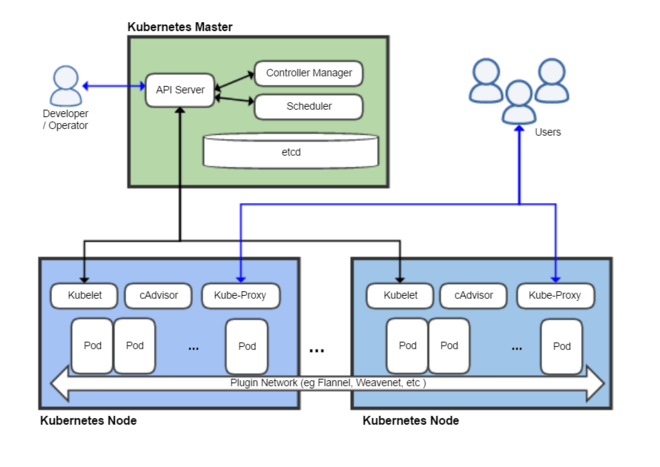
\includegraphics[width=0.8\columnwidth]{images/kubernetes01.png}
	\caption{Estructura de un clúster de Kubernetes \cite{BOOK02}.}
	\label{fig:kub01}
\end{figure}
\par Un clúster de Kubernetes es un conjunto de recursos informáticos, de almacenamiento y de red donde los pods se despliegan, administran y escalan. El grupo (clúster) esta formado por nodos conectados a través de una red "plana", en la que cada nodo y pod pueden comunicarse entre sí. Un tamaño de clúster de Kubernetes típico varía de 1 a 200 nodos \cite{BOOK04}. Los componentes de un clúster de Kubernetes y sus funciones principales se presentan a continuación:\\ 

\textbf{Pods:} Un pod es un grupo de uno o más contenedores estrechamente relacionados que se ejecutan juntos en el mismo nodo de trabajo y en los mismos \textit{namespaces} de Linux. Cada pod es como una máquina lógica con su propia IP, nombre de host, procesos, etc., ejecutando una sola aplicación. Dichos pods tienen volúmenes, los cuales son directorios, posiblemente con algunos datos en estos, que es accesible para los contenedores del pod. La aplicación puede ser un solo proceso ejecutándose en un solo contenedor o varios procesos de soporte adicionales, cada uno ejecutándose en su propio contenedor. Todos los contenedores en un pod parecerán estar ejecutándose en la misma máquina lógica, mientras que los contenedores en otros pods, incluso si se están ejecutando en el mismo nodo de trabajo, parecerán estar ejecutándose en uno diferente  \cite{BOOK01}. En la figura \ref{fig:kub02} se muestra un esquema que ayuda a comprender la relación entre contenedores, pods y nodos. \\


\begin{figure}[htpb!]
	\centering
	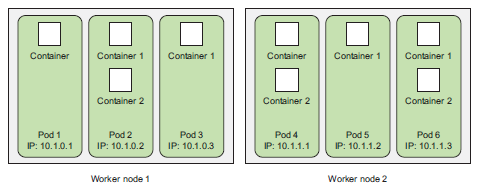
\includegraphics[width=0.8\columnwidth]{images/kubernetes02.PNG}
	\caption{Relación entre contenedores, pods y nodos \cite{BOOK01}.}
	\label{fig:kub02}
\end{figure}

\textbf{Controladores:} El controlador principal es el controlador de replicación, que funciona para garantizar que se ejecute un número específico de réplicas de pod en cualquier momento. Se asegura de que un pod o un conjunto homogéneo de pods esté siempre activa y disponible. Cuando hay demasiados pods, el controlador de replicación terminará los pods innecesarios. Si el número de pods es demasiado bajo, el controlador de replicación iniciará más pods. Lo hace utilizando métricas proporcionadas por la aplicación, como la utilización de la CPU. La ventaja de tener los pods controlados por el controlador de replicación es que si un pod falla por algún motivo, creará automáticamente otro pod para reemplazar uno que falla. Los controladores de replicación brindan la capacidad de escalar pods en una flota de máquinas y garantizar que el número deseado de Pods esté siempre en funcionamiento. Existen otras funciones a nivel del clúster que se manejan con otros controladores, por ejemplo, la gestión de puntos finales de servicio, se maneja mediante el controlador de puntos finales, y la gestión del ciclo de vida del nodo, se maneja mediante el controlador de nodo. Cada uno de estos controladores se ejecutan en un solo proceso llamado Controller Manager. \cite{BOOK02,BOOK04}.\\

\textbf{Servicios:} Un servicio de Kubernetes es un recurso que crea un único punto de entrada constante a un grupo de pods que brindan el mismo servicio. Cada servicio tiene una dirección IP y un puerto que nunca cambian mientras el servicio existe. Los clientes pueden abrir conexiones a esa IP y puerto, y esas conexiones se enrutan a uno de los pods que respaldan ese servicio. De esta manera, los clientes de un servicio no necesitan conocer la ubicación de los Pods individuales que brindan el servicio, lo que permite que esos pods se muevan alrededor del clúster en cualquier momento \cite{BOOK01}.En figura \ref{fig:kub03} se presenta el esquema de un ejemplo de servicio.\\

\begin{figure}[htpb!]
	\centering
	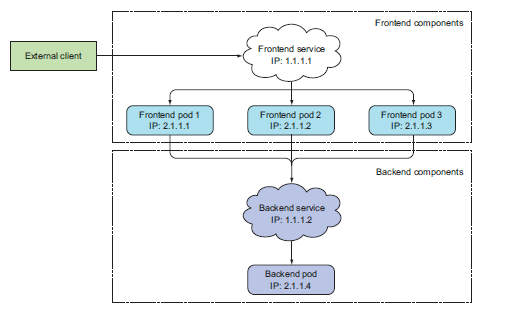
\includegraphics[width=0.8\columnwidth]{images/kubernetes03.png}
	\caption{Esquema ejemplo de un servicio. Los clientes internos y externos generalmente se conectan a Pods a través de servicios \cite{BOOK01}.}
	\label{fig:kub03}
\end{figure}

\textbf{etcd:} etcd es un almacén de valores clave, distribuido y consistente para la configuración compartida y el descubrimiento de servicios, enfocado en ser simple, seguro, rápido y confiable. Etcd utiliza el algoritmo de consenso Raft para lograr tolerancia a fallas y alta disponibilidad. Proporciona la capacidad de ``observar'' los cambios, permitiendo una rápida coordinación entre los componentes de Kubernetes. Todo el estado del clúster persistente se almacena en etcd \cite{BOOK04}.\\


\textbf{Kubernetes API Server:} El apiserver es responsable de servir la API de Kubernetes y los componentes del clúster de proxy, como la interfaz de usuario web de Kubernetes. El apiserver expone una interfaz REST que procesa operaciones como la creación de pods, los servicios y la actualización de los objetos correspondientes en etcd \cite{BOOK04}.\\

\textbf{Planificador:} Se encarga de observar el apiserver en busca de pods no programados y los programa en nodos saludables según los requisitos de recursos \cite{BOOK04}.\\

\textbf{Container runtime:} 

Software encargado de ejecutar y manejar los contenedores, se ejecuta en cada nodo para llevar a cabo el inicio de las imágenes de contenedores y administrar su funcionamiento. Docker es el container runtime mas común, y es controlado localmente a través de su API por Kubelet \cite{BOOK04}.\\



\textbf{Kubelet:} Cada nodo ejecuta el Kubelet que es responsable del registro del nodo y la gestión de los pods. El Kubelet observa el servidor de la API de Kubernetes en busca de pods para crear, según lo programado por el planificador, o pods para eliminar, en función de los eventos del clúster. Kubelet también maneja la utilización de recursos de informes y la información del estado de salud para un nodo específico y los pods que está ejecutando \cite{BOOK04}.\\

\textbf{Proxy:} Cada nodo también ejecuta un proxy de red simple con soporte para el reenvío de flujo TCP y UDP, a través de un conjunto de pods como se define en la API de Kubernetes \cite{BOOK04}.\\


%%%%%%%%%%%%%%%

% %%%%%%%%%%%%%%%

\section{Fault Injection (inyección de fallas)}

\par Es posible que un sistema no siempre realice la función para la que está destinado. Las causas y consecuencias de las desviaciones de la función esperada de un sistema se denominan factores de confiabilidad \cite{LIB05}:
\begin{itemize}
    \item La \textbf{falla} es un defecto físico, imperfección o interrupción que ocurre dentro de algún componente de hardware o software.
    \item El \textbf{error} es una medida de la diferencia estimada entre el valor observado y su valor verdadero.
    \item El \textbf{fracaso} es el incumplimiento de alguna acción que se debe o se espera.
\end{itemize}


\par Cuando una falla causa un cambio en una etapa de la máquina, se produce un error. Una falla localizada en un código o circuito especifico, puede provocar múltiples errores desde el sitio de falla que se propagan por todo el sistema. Cuando los mecanismos de tolerancia a fallas detectan un error, pueden iniciar varias acciones para manejar las fallas y contener sus errores. De lo contrario, el sistema finalmente funciona mal y se produce un fracaso.\\

\par No es suficiente diseñar un circuito con un conjunto de mecanismos de detección de fallas cuidadosamente seleccionados, para garantizar poder evitar los efectos críticos de las fallas, ya que los mecanismos implementados en general no pueden detectar todas las fallas posibles. En la fase del diseño de inyección de fallas debe establecerse un equilibrio entre la cobertura de fallas obtenida para los diferentes tipos de fallas y los diversos costos inducidos. La evaluación final de la confiabilidad del circuito y del sistema se realiza de manera clásica mediante inyección de fallas en un prototipo del sistema \cite{LIB05}.\\
\par Fault injection o la inyección de fallas, proporciona un método para evaluar la confiabilidad de un sistema bajo prueba. Consiste en insertar fallas en un sistema y monitorearlo para determinar su comportamiento en respuesta a una falla. Se han propuesto y experimentado varias técnicas de inyección de fallas. Mediante la inyección de un rango definido de fallas, se intenta determinar si la respuesta del sistema coincide con sus especificaciones. Normalmente, las fallas se inyectan en estados y puntos del sistema, previamente determinados en un análisis inicial de este \cite{LIB05}.\\

\par Las técnicas de inyección de fallas posibilitan tanto la eliminacion de fallas (la corrección de posibles deficiencias de tolerancia a fallas en el sistema), como el pronóstico de fallas (la evaluación de la distribución de cobertura -factor de cobertura y latencia- proporcionada por el sistema probado). Para la eliminación de fallas, la prueba debe estar dirigida a lograr una alta cobertura de las posibles configuraciones del sistema a validar. La selección de las fallas/errores a aplicar y los errores a propagar se basa principalmente en el análisis del modelo que describe el sistema y el flujo de información en la simulación del sistema \cite{LIB05}.

\subsection{Entorno de inyección de fallas}

\par Un entorno de inyección de fallas generalmente consta de los siguientes componentes \cite{LIB07}:
\begin{itemize}
    \item Inyector de fallas (\textit{Fault Injector}): inyecta fallas en el sistema de destino mientras ejecuta comandos del generador de carga de trabajo.
    \item Biblioteca de fallas (\textit{Fault Library}): almacena tipos, ubicaciones y tiempos de las fallas, asi como semántica de hardware y estructuras de software apropiadas.
    \item Generador de carga de trabajo (\textit{Workload Generator}): genera la carga de trabajo para el sistema de destino.
    \item Biblioteca de carga de trabajo (\textit{Workload Library}): almacena cargas de trabajo de muestra para el sistema de destino.
    \item Controlador (\textit{Controller}): controla el experimento.
    \item Monitor: realiza un seguimiento de la ejecución de los comandos e inicia la recopilación de datos siempre que sea necesario.
    \item Recopilador de datos (\textit{Data Collector}): realiza la recopilación de datos en línea.
    \item Analizador de datos (\textit{Data Analyzer}): realiza el procesamiento y análisis de datos.
\end{itemize}

\begin{figure}[htpb!]
	\centering
	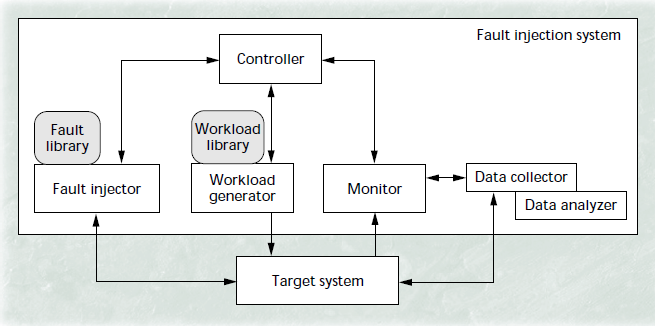
\includegraphics[width=0.8\columnwidth]{images/fi01.PNG}
	\caption{Entorno clásico de la inyección de fallas \cite{LIB07}.}
	\label{fig:fi01}
\end{figure}

\par En la Figura \ref{fig:fi01} se presenta un entorno clásico de inyección de fallas, el cual consiste en: el sistema de destino, un inyector de fallas, la biblioteca de fallas, un generador de carga de trabajo y la biblioteca de carga de trabajo.

\subsection{Tipos de Inyección de Fallas}

\par En general la inyección de fallas se utiliza para probar la tolerantes a fallas en sistemas o componentes. La inyección de fallas prueba la detección de fallas, el aislamiento de fallas y las capacidades de reconfiguración y recuperación. La elección entre inyección de fallas de hardware o de software, depende del tipo de fallas que interesen y del esfuerzo requerido para crearlas. Por ejemplo, si se está interesado en fallas atascadas (fallas que fuerzan un valor permanente en un punto de un circuito), es preferible utilizar un inyector de fallas de hardware, ya que el podría identificar la ubicación de la falla y controlarla. La inyección de fallas permanentes utilizando métodos de software, dependiendo de la falla, provoca una sobrecarga elevada o es imposible realizar. Sin embargo, si se está interesado en la corrupción de datos, el enfoque de software podría ser suficiente \cite{LIB07}.

\subsubsection{Inyección de Fallas por Hardware}
\par Las fallas físicas/de hardware que surgen durante la operación del sistema se clasifican mejor por su duración: permanente, transitoria o intermitente \cite{LIB05}.\\
\par La inyección de fallas en hardware consiste en agregar al sistema bajo análisis, un hardware de prueba especialmente diseñado para la inyección de fallas y examinar los efectos. Dependiendo de las fallas y sus ubicaciones, los métodos implementados de inyección de fallas por hardware se dividen en dos categorías \cite{LIB05}:
\begin{itemize}
    \item Inyección de falla por hardware con contacto. El inyector tiene contacto físico directo con el sistema objetivo, produciendo cambios de voltaje o corriente externamente al chip objetivo, por ejemplos los métodos que usan sondas y sockets a nivel de pin.
    \item Inyección de falla por hardware sin contacto. El inyector no tiene contacto físico directo con el sistema de destino. En cambio, una fuente externa produce algún fenómeno físico, como interferencia electromagnética o radiación de partículas pesadas, causando corrientes espurias dentro del chip objetivo.
\end{itemize}
\par Generalmente se modelan métodos de hardware en modelos de fallas de bajo nivel, por ejemplo, una falla de puente podría ser un cortocircuito. El inyector de fallas por hardware desencadena fallas y monitorea su impacto, proporcionando así alta resolución temporal y baja perturbación. Normalmente, el inyector de fallas por hardware desencadena fallas después de un tiempo específico controlado en un temporizador de hardware o después de haber detectado un evento, como una dirección especificada en el bus de direcciones \cite{LIB07}.\\

\subsubsection{Inyección de Fallas por Software}

\par Las fallas de software son generalmente consecuencia de un diseño incorrecto en la especificación o en el momento de la codificación. Muchas de estas fallas están latentes en el código y se muestran solo durante la operación, especialmente bajo cargas de trabajo pesadas o inusuales y contextos de tiempo determinados. Como son el resultado de un mal diseño, se podría suponer que todas las fallas del software serían permanentes, sin embargo, la práctica a demostrado fallas de software con comportamiento transitorio: a veces cuando se produce un mal comportamiento del sistema, este no se puede volver a observar, incluso si se tiene mucho cuidado de repetir la situación en la que se produjo. Este comportamiento se denomina comúnmente falla del sistema \cite{LIB05}.\\


\par Las fallas pueden crearse en los distintos pasos del proceso de desarrollo de un software: definición de requisitos, especificaciones de requisitos, diseño, implementación y pruebas.\\


\par En los últimos años, los investigadores han tomado más interés en desarrollar herramientas de inyección de fallas implementadas por software. Las técnicas de inyección de fallas por software son atractivas porque no requieren hardware costoso. Además, pueden usarse para apuntar a aplicaciones y sistemas operativos, lo cual es difícil de hacer con la inyección de fallas por hardware. Si el objetivo es una aplicación, el inyector de fallas se inserta en la aplicación o se coloca entre la aplicación y el sistema operativo. Si el objetivo es el sistema operativo, el inyector de fallas debe estar integrado en el sistema operativo, ya que es muy difícil agregar una capa entre la máquina y el sistema operativo \cite{LIB07}.\\

\par Los métodos de implementación de inyección de fallas, se pueden separar según siguientes los modelos de fallas:

\begin{itemize}
    \item Corrupción de datos de almacenamiento (como registro, memoria y disco).
    \item Corrupción de datos de comunicación (como bus y red de comunicación).
    \item Manifestación de defectos de software (como nivel de máquina y niveles superiores).
\end{itemize}.


\par Los tipos de inyección de fallas, se establecen los siguientes mecanismos:
\begin{itemize}
    \item \textbf{Inyección de fallas basada en hardware}: estas se realizan a nivel físico, perturbando el hardware con parámetros del entorno (radiación de iones pesados, interferencias electromagnéticas, etc.), inyectando caídas de voltaje en los rieles de alimentación del hardware (perturbaciones de la fuente de alimentación), modificando el valor de los pines del circuito o inyectando una falla vía láser. \cite{LIB07}.
    \item \textbf{Inyección de fallas basada en software}: en este mecanismo consiste en reproducir a nivel de software los errores consecuencias de fallas en el hardware \cite{LIB05}.
    \item \textbf{Inyección de fallas híbrida}: este mecanismo utiliza un enfoque que combina una implementación de fallas inyectadas por software y por hardware \cite{LIB07}.\\
\end{itemize}
\par Desde otro punto de vista, los mecanismos de inyección de fallas pueden agruparse en mecanismos invasivos y no invasivos. El problema con los sistemas suficientemente complejos, particularmente los que dependen del tiempo, independientemente de la falla inyectada, es que puede ser imposible eliminar la huella del mecanismo de prueba del comportamiento del sistema. Los mecanismos invasivos son aquellos que dejan una huella durante la prueba. Los mecanismos no invasivos pueden enmascarar su presencia, para evitar cualquier otro efecto en el sistema que no sean las fallas que inyectan \cite{LIB05}.\\
\vspace{\baselineskip}

\par En la tabla \ref{tab:tablafi} se presenta un resumen de las ventajas y desventajas de los distintos mecanismos de inyección de fallas.\\


\begin{table}[ht!]
\centering
\caption{Tabla comparativa entre los principales mecanismos de inyección de fallas \cite{LIB05}.}
\vspace{0.5\baselineskip}
\resizebox{\linewidth}{!}{%
\huge
\begin{tabular}{|l|c|c|}
\hline
\rowcolor[HTML]{34CDF9} 
{\color[HTML]{000000} \textbf{Mecanismos}} & \multicolumn{1}{l|}{\cellcolor[HTML]{34CDF9}{\color[HTML]{000000} \textbf{Ventajas}}} & \multicolumn{1}{l|}{\cellcolor[HTML]{34CDF9}{\color[HTML]{000000} \textbf{Desventajas}}} \\ \hline
{\color[HTML]{000000} \textbf{Basado en Hardware}} & \begin{tabular}[c]{@{}c@{}}
    \tabitem Puede acceder a ubicaciones a las que \\ es difícil acceder por otros medios.\\ 
    \tabitem Alta resolución de tiempo para activación \\ y supervisión de hardware.\\ Muy adecuado para los modelos de \\ fallas de bajo nivel.\\ 
    \tabitem Los experimentos son rápidos.\\ 
    \tabitem No se requiere desarrollo o validación \\ del modelo.\\ \tabitem Capaz de modelar fallas permanentes a \\ nivel de pin.
\end{tabular} & \begin{tabular}[c]{@{}c@{}}
    \tabitem Puede introducir un alto riesgo de daños para \\ el sistema inyectado.\\ 
    \tabitem El alto nivel de integración del dispositivo, \\ el circuito híbrido de múltiples chips y las \\ tecnologías de empaquetado denso limitan la \\ accesibilidad a la inyección.\\ 
    \tabitem Baja portabilidad y observabilidad.\\ Conjunto limitado de puntos de inyección \\ y conjunto limitado de fallas inyectables.\\ 
    \tabitem Requiere hardware de propósito especial \\ para realizar los experimentos de inyección \\ de fallas.
\end{tabular} \\ \hline
{\color[HTML]{000000} \textbf{Basado en Software}} & \begin{tabular}[c]{@{}c@{}}
    \tabitem Puede ser dirigido a aplicaciones y sistemas \\ operativos.\\ 
    \tabitem Los experimentos se pueden ejecutar en tiempo \\ casi real.\\ 
    \tabitem No requiere ningún hardware de propósito \\ especial; baja complejidad, bajo desarrollo y \\ bajo costo de  implementación.\\ 
    \tabitem No se requiere desarrollo o validación del modelo.\\ Se puede ampliar para nuevas clases de fallas.
\end{tabular} & \begin{tabular}[c]{@{}c@{}}
    \tabitem Conjunto limitado de instantes de inyección.\\ 
    \tabitem No puede inyectar fallas en ubicaciones \\ inaccesibles para el software.\\ 
    \tabitem Requiere una modificación del código fuente \\ para admitir la inyección de falla.\\ 
    \tabitem Observabilidad y controlabilidad limitadas.\\ 
    \tabitem Muy difícil modelar fallas permanentes.
\end{tabular} \\ \hline
\end{tabular}%
}
\label{tab:tablafi}
\end{table}

\subsection{Inyección de fallas en Servicios Web y Redes  }

\par Dada la importancia de los servicios web en la actualidad, se requieren métodos y herramientas de prueba para garantizar que se desplieguen servicios de software robustos y tolerantes a fallas. Se necesitan pruebas no solo para descubrir problemas existentes en los sistemas, sino también para proporcionar a los usuarios métricas para comparar soluciones basadas en servicios similares \cite{LIB19}.\\

\par La aplicación de inyección de fallas en sistemas distribuidos se ha concentrado en los sistemas basados en Llamadas a Procedimiento Remoto (\textit{RPC}) estrechamente acoplados. Al definir un método de evaluación para arquitecturas orientadas a servicios (o \textit{SOA} por sus siglas en inglés), nos enfrentamos a un nuevo conjunto de desafíos que requieren soluciones diferentes. Los desafíos principales son: 1) mayor probabilidad de falla de la red; 2) mayores niveles de seguridad y encriptación; 3) plataforma de naturaleza mas genérica, que soporte múltiples lenguajes de programación; 4) restricciones de tiempo y operaciones del servicio web de naturaleza asincrónica. \cite{LIB19}.\\

\par Existe mucha mas investigación en el desarrollo de herramientas de inyección de falla implementada por software (\textit{SWIFI Software Implemented Fault Injection}), que en la inyección de falla implementada por hardware. Esto se debe en parte a que una herramienta SWIFI no requiere ningún hardware costoso. SWIFI también permite que sistemas específicos que se ejecutan en el hardware de destino, sean dirigidos efectivamente sin inyectar fallas en otras partes del sistema \cite{LIB19}.\\

\subsubsection{Calidad de Servicio (\textit{QoS})}

\par QoS cubre una amplia gama de técnicas que se combinan para formar métricas sobre la calidad de un servicio web ofrecido por un sistema. En este punto, será útil definir la mayoría de los términos de QoS:
\begin{itemize}
    \item Disponibilidad: es el aspecto de calidad de si un servicio web está presente y listo para usar. Se representa como la probabilidad de que un servicio web esté disponible. Por ejemplo, la disponibilidad puede verse afectada por el tiempo para completar una operación anterior, la carga de un servicio en particular, etc.
    \item Accesibilidad: es el aspecto de calidad que representa el grado en que el servicio web es capaz de atender una solicitud. Un servicio puede estar disponible pero no accesible. Por ejemplo, la solicitud inicial puede aceptarse pero puede no procesarse debido a alguna otra dependencia de un servicio no disponible. La accesibilidad se puede mejorar aumentando la escalabilidad del sistema.
    \item Integridad: es la calidad del servicio web que asegura la corrección de cualquier interacción. Si una transacción falla, los datos deben permanecer en un estado coherente.
    \item Rendimiento: es el aspecto de calidad que refiere a la efectividad de un servicio web y la latencia. El rendimiento es el número de solicitudes atendidas en un período determinado y la latencia es el tiempo necesario para atender una solicitud. El objetivo es producir un sistema de alto rendimiento pero baja latencia. El rendimiento y la latencia pueden verse afectados por factores tales como la velocidad del procesador, la eficiencia del código, el tiempo de transferencia de la red, etc.
    \item Fiabilidad: es el aspecto de calidad relacionado a la capacidad de mantener la calidad del servicio. Una medida de confiabilidad es el número de fallas durante un período de tiempo dado.
    \item Regulatorio: es el aspecto de calidad relacionado al cumplimiento de las normas, leyes, estándares y especificaciones establecidas. Puede tener un efecto en áreas como la disponibilidad, el rendimiento y la confiabilidad a través de los acuerdos de nivel de servicio (\textit{SLA}).
    \item Seguridad: es el aspecto de calidad que refiere a la confidencialidad para las partes que utilizan un servicio. Puede estar influenciada por factores reguladores. También puede afectar el rendimiento debido a la sobrecarga adicional incurrida en la implementación de mecanismos de seguridad.
\end{itemize}

\subsubsection{Inyección de falla a nivel de red}

\par La inyección de falla a nivel de red se refiere a la corrupción, pérdida o reordenamiento de mensajes en la interfaz de red. Es posible utilizar herramientas de inyección de fallas implementadas por software, para inyectar fallas al instrumentar la pila de protocolos del sistema operativo, pero esto corre el riesgo de ser detectado y rechazado por la pila de protocolos de los sistemas receptores, por lo tanto, es preferible inyectar la falla en el nivel de aplicación. Generalmente, las fallas inyectadas se basan en la corrupción de la información del encabezado del mensaje y la inyección de errores de bits aleatorios \cite{LIB19}.\\
%%%%%%%%%%%%%%

\section{Chaos Engineering (ingeniería del caos)}
\par Hace treinta años, Jim Gray señaló que ``una forma para mejorar la disponibilidad es utilizar hardware y software probados y luego dejarlos en paz''. Para las empresas que brindan servicios a través de Internet, ``dejarlos en paz'' no es una opción. Los proveedores de servicios, deben realizar cambios continuamente para aumentar el valor del servicio, por ejemplo agregar nuevas funciones y mejorar el rendimiento. En Netflix, los ingenieros introducen nuevos códigos en producción y modifican los parámetros de configuración de tiempo de ejecución cientos de veces al día. La disponibilidad sigue siendo importante: un cliente que no puede ver un vídeo debido a una interrupción del servicio, podría no ser un cliente por mucho tiempo. Pero para lograr altos niveles de disponibilidad, se necesita aplicar un enfoque diferente al que Gray abogó \cite{LIB02}.\\
\par Netflix ha estado ejecutando un servicio interno llamado Chaos Monkey, que selecciona aleatoriamente instancias de máquinas virtuales, que alojan los servicios de producción y los finaliza. El propósito de Chaos Monkey era alentar a diseñar servicios de software, que puedan soportar fallas de instancias individuales. Chaos Monkey sólo está activo durante las horas normales de trabajo, para que los ingenieros puedan responder rápidamente si un servicio falla debido a la finalización de una instancia. Chaos Monkey demostró ser exitoso y este éxito los alentó a extender el enfoque de inyectar fallas en el sistema de producción para mejorar la confiabilidad \cite{LIB02}.\\
\par La ingeniería del caos, la inyección de fallas y las pruebas de fallas tienen una gran superposición en las preocupaciones y muchas veces también en las herramientas. Por ejemplo, muchos experimentos de la ingeniería del caos, se basan en la inyección de fallas para introducir el efecto que se está estudiando. La diferencia principal entre la ingeniería del caos y la inyección de fallas, es que la primera es una práctica para generar nueva información, mientras que la inyección de fallas es un enfoque específico para probar una condición. Cuando se desee explorar las muchas formas en que un sistema complejo puede comportarse mal, inyectar fallas de comunicación como latencia y errores es un buen enfoque. A continuación se presentan algunos ejemplos de entradas para experimentos \cite{LIB06}:
\begin{itemize}
    \item Simulando la falla de toda una región o centro de datos.
    \item Eliminar parcialmente los temas de Kafka en una variedad de instancias para recrear un problema que ocurrió en la producción.
    \item Inyección de latencia entre servicios para un porcentaje selecto de tráfico durante un período de tiempo predeterminado.
    \item Caos basado en funciones (inyección en tiempo de ejecución): provoca aleatoriamente que las funciones arrojen excepciones.
    \item Inserción de código: Agregar instrucciones al programa de destino y permitir la inyección de fallas antes de ciertas instrucciones.
    \item Viaje en el tiempo: forzar a los relojes del sistema a sincronizarse entre sí.
    \item Ejecutar una rutina en el código del controlador emulando errores de E/S.
    \item Maximizar los núcleos de CPU en un clúster Elasticsearch.
\end{itemize}

\par Se puede establecer una distinción importante entre las pruebas y la experimentación. En las pruebas, se hace una afirmación: dadas unas condiciones específicas, un sistema emitirá una salida específica. Las pruebas suelen ser binarias y determinan si una propiedad es verdadera o falsa. Estrictamente hablando, esto no genera nuevos conocimientos sobre el sistema, solo asigna valencia a una propiedad conocida del mismo. La experimentación genera nuevos conocimientos y a menudo sugiere nuevas vías de exploración.\\

\par Organizaciones como Amazon, Google, Microsoft y Facebook, estaban aplicando técnicas similares para probar la resistencia de sus propios sistemas. Es una creencia de que estas actividades forman parte de una disciplina que está surgiendo en la industria, que se llama Ingeniería del Caos. Específicamente, la ingeniería del Caos es la disciplina de experimentar en un sistema distribuido, para generar confianza en su capacidad de soportar condiciones turbulentas en la producción. Estas condiciones pueden ser desde una falla de hardware hasta un aumento inesperado en el número de solicitudes de clientes y un valor con formato incorrecto en un parámetro de configuración en tiempo de ejecución. La Ingeniería del Caos se usa para referirse a este enfoque, discutir los principios subyacentes y cómo usarlo para realizar experimentos \cite{LIB02}.\\
\subsection{Principios de la ingeniería del caos}
\par La ingeniería del caos se basa en la ejecución de experimentos. Como en otras disciplinas experimentales, diseñar un experimento requiere especificar \cite{LIB02}:
\begin{itemize}
    \item Hipótesis.
    \item Variables independientes.
    \item Variables dependientes.
    \item Contexto.
\end{itemize}

\par Los cuatro principios fundamentales del enfoque de la ingeniería del caos para diseñar experimentos son \cite{LIB02}:
\begin{itemize}
    \item Construir una hipótesis alrededor del comportamiento de estado estable.
    \item Variar los eventos del mundo real.
    \item Realizar experimentos en producción.
    \item Automatizar los experimentos para correr continuamente.
\end{itemize}

\subsubsection{Hipótesis sobre el estado estable}

\par El término ``estado estable'', se usa para referirse a una propiedad como la temperatura interna del cuerpo, donde el sistema tiende a mantener esa propiedad dentro de un cierto rango o patrón. El objetivo en la identificación del estado estable, es desarrollar un modelo que caracterice el estado estable del sistema en función de los valores esperados. Para cualquier sistema complejo, habrá muchas partes móviles, muchas señales y muchas formas de salida. Es necesario distinguir de manera muy general entre los comportamientos sistémicos que son aceptables y los comportamientos que no son deseables \cite{LIB06}.\\

\par  Las métricas del sistema pueden ser útiles para ayudar a solucionar problemas de rendimiento y en algunos casos, errores funcionales. Las métricas son como los signos vitales del sistema.\\
\par Dependiendo del dominio, sus métricas pueden variar de manera menos predecible con el tiempo. Por ejemplo en un sitio web de noticias, el tráfico puede estar marcado por picos, cuando ocurre un evento de noticias de gran interés para el público en general. En algunos casos, el pico puede ser predecible y en otros puede ser imposible de predecir de antemano. En este tipo de casos, caracterizar el comportamiento en estado estable del sistema será más complejo. De cualquier manera, caracterizar el comportamiento en estado estable, es una condición previa necesaria para crear una hipótesis significativa al respecto \cite{LIB06}.\\

\par Cada vez que se realiza un experimento de caos, se debe tener una hipótesis en mente sobre lo que se cree que será el resultado del experimento. Puede ser tentador someter el sistema a diferentes eventos (por ejemplo, aumentar la cantidad de tráfico), para ``ver qué sucede''. Sin embargo, sin tener una hipótesis previa en mente, puede ser muy difícil sacar conclusiones si no se sabe qué se busca en los datos. Una vez seleccionadas las métricas y una comprensión de su comportamiento en estado estable, ellas pueden ser usadas para definir las hipótesis del experimento. Se debe considerar cómo cambiará el comportamiento del estado estable cuando se inyectan diferentes tipos de eventos en el sistema. Luego, se mide el cambio en el comportamiento del estado estable. Incluso cuando se define el modelo del comportamiento de estado estable, es necesario definir cómo se van a medir las desviaciones de este modelo \cite{LIB06}.

\subsubsection{Variar eventos del mundo real}

\par Todos los sistemas, tanto los simples como los complejos, están sujetos a eventos y condiciones impredecibles, tales como aumento de la carga, mal funcionamiento del hardware, implementación de software defectuoso y la introducción de datos no válidos \cite{LIB06}. Estos eventos y condiciones impredecibles se materializan generalmente a partir de:
\begin{itemize}
    \item Fallas de hardware.
    \item Errores funcionales.
    \item Errores de transmisión de estado (por ejemplo, inconsistencia de estados entre los nodos emisor y receptor).
    \item Latencia de red y partición. 
    \item Grandes fluctuaciones en la entrada (subida y bajada) y reintento.
    \item Agotamiento de recursos.
    \item Combinaciones inusuales o impredecibles de comunicación entre servicios.
    \item Fallos bizantinos (por ejemplo, un nodo que cree que tiene los datos más actuales cuando en realidad no los tiene).
    \item Condiciones de carrera.
    \item Mal funcionamiento de dependencias.
\end{itemize}

\par Quizás lo más interesante, son las combinaciones de los eventos enumerados anteriormente, las cuales causan comportamientos sistemáticos adversos. Aunque no es posible prevenir las amenazas a la disponibilidad, si es posible mitigarlas. La decisión sobre que eventos se van a inducir, se realiza comparando la frecuencia y el impacto de ellos con sus costos y complejidades \cite{LIB06}.

\subsubsection{Realizar experimentos en producción}

\par Un principio común en las pruebas clásicas, es identificar los errores lo más lejos posible de la producción. En Ingeniería del Caos, la estrategia se invierte: los experimentos se ejecutan lo más cerca posible del entorno de producción. Una forma ideal, seria ejecutar todos los experimentos directamente en el entorno de producción.\\

\par Durante las pruebas tradicionales de software se verifica la corrección del código, mientras que en los experimentos de la ingienería del caos, interesa el comportamiento de todo el sistema en general. Si bien el código es una parte importante del sistema, el sistema es mucho más complejo que el código.\\

\par Cuando un sistema despliega un servicio, el recibirá  diferentes tipos de solicitudes de sus usuarios.  El sistema puede intentar construir un modelo sintético de entrada de usuario, pero cuando los usuarios se comportan de una forma diferente a lo esperado, el sistema de producción queda sujeto a entradas no reportadas en las pruebas con datos sintéticos. La única forma de generar confianza en el sistema en cuestión, es experimentar con la entrada real recibida por el entorno de producción \cite{LIB06}.

\subsubsection{Automatizar los experimentos para ejecutar continuamente}

\par En los sistemas modernos complejos no se puede conocer a priori, cuales cambios en el entorno de producción alterarán los resultados de un experimento de caos. Debido a esto, se debe asumir que cualquier cambio en el entorno de producción pueden afectar a los experimentos. En realidad la producción esta en un estado de cambio perpetuo, a partir del estado compartido, el almacenamiento en caché, la gestión de configuración dinámica, la entrega continua, el escalado automático y el código de tiempo. Como resultado, la confianza decae con el tiempo \cite{LIB06}.\\

\par Idealmente, los experimentos deberían realizarse con cada cambio. Cuando se descubre un nuevo riesgo y el operador esta convencido de que el cambio desplegado es la causa, se debe poder elegir bloquear el despliegue del cambio y priorizar una solución. Este enfoque posibilita información del inicio y la duración de los riesgos de disponibilidad en la producción. Otro enfoque son los ejercicios anuales, ellos conducen a investigaciones más difíciles que esencialmente comienzan desde cero y no proporcionan una idea fácil de cuánto tiempo ha estado en producción el problema potencial. Una buena practica es configurar experimentos que se ejecuten de forma regular automáticamente \cite{LIB06}.

\subsection{Diseñando experimentos}
\par En la ingeniería del caos es fundamental la ejecución de experimentos, para generar confianza en el comportamiento del sistema. En base a esto, un experimento se define a través de los siguientes pasos \cite{LIB02, LIB06}:
\begin{itemize}
    \item Primero se define el estado estable, que es un resultado medible del sistema que indica un comportamiento normal.
    \item Se hipotetiza que este estado estable continuará tanto en el grupo de control como en el grupo experimental.
    \item Se introducen variables que reflejen eventos del mundo real, por ejemplo servidores que se bloquean, discos duros que funcionan mal, conexiones de red que se cortan, otros.
    \item Luego se intenta refutar la hipótesis, a partir de diferencias del estado estable en el grupo de control y en el grupo experimental.
    \item Se analizan los resultados, aumenta el alcance y automatiza.
\end{itemize}

\par La ingeniería del caos todavía es un campo muy joven y sus técnicas y herramientas asociadas todavía están evolucionando.

\section{Herramientas de Configuración}
\par  Actualmente es necesario que los administradores incorporen los servidores nuevos, a través de una intervención minina o automáticamente, en lugar de desplegar, parchear y destruir cada servidor a mano. De esta necesidad surge la gestión de configuración de software, la cual tiene una definición tradicional a partir de las siguientes funciones específicas:
\begin{itemize}
    \item Identificación de la configuración.
    \item Cambio de control.
    \item Estado contable.
    \item Despliegue.
    \item Auditoría de la configuración.
\end{itemize}

\par Estas funciones se han descrito durante mucho tiempo en los marcos y estándares de la industria, ellas posibilitan definir las siguientes metas en la gestión de la configuración por software \cite{BOOK14}: Identificación de configuraciones, elementos de configuración y líneas de base, control de configuración, contabilidad de estado de configuración, seguimiento de defectos, entre otras. Las herramientas actualmente pueden modelar y administrar recursos virtuales basados en la nube, incluidos dispositivos virtuales, unidades de almacenamiento y paquetes de software. Los roles y responsabilidades de los actores se fusionaron con los desarrolladores, que ahora pueden instanciar dinámicamente servidores virtuales y recursos relacionados. Tres de las mas relevantes herramientas de gestión de configuración utilizadas actualmente son:
%%%%%%%%%%%%%%%%%%%%%
\subsection{Ansible}

\par Ansible comúnmente se describe como una herramienta de administración de configuración y generalmente se menciona en la misma categoría que Chef, Puppet y Salt. En la gestión de configuración, generalmente se escribe algún tipo de descripción de estado para algunos servidores y luego se utiliza una herramienta para garantizar que los servidores estén en ese estado; esto es que los paquetes correctos están instalados, los archivos de configuración contienen los valores esperados y permisos esperados, se están ejecutando los servicios correctos, etc. Ansible, al igual que otras herramientas de administración de configuración, expone un lenguaje específico de dominio (o DSL por sus iniciales en inglés) que se utiliza para describir el estado de los servidores \cite{BOOK13}.\\



\par Las principales ventajas de Ansible son su simplicidad y facilidad de uso. Otras ventajas destacadas son seguridad y  confiabilidad, el uso de OpenSSH para el transporte y un lenguaje diseñado para auditar por los humanos. Ansible funciona al enviar los cambios a todos sus servidores de manera predeterminada y no requiere la instalación de ningún software adicional en sus servidores, por lo tanto, no requiere una huella de memoria adicional ni un demonio adicional para administrar, a diferencia de la mayoría de las otras herramientas de administración de configuración \cite{BOOK13}.\\

\par En la Figura \ref{fig:ansible01} se presenta un modelo de la utilización de Ansible. en este modelo un usuario está usando Ansible para configurar servidores web. En Ansible, un script se llama Playbook; un Playbook describe qué hosts (que Ansible llama servidores remotos) configurar y una lista ordenada de tareas para realizar en estos hosts. El Nodo maestro,analiza y recopila datos de cada servidor y los Playbooks son enviados hacia cada nodo. \cite{BOOK13}.\\
\begin{figure}[htpb!]
	\centering
	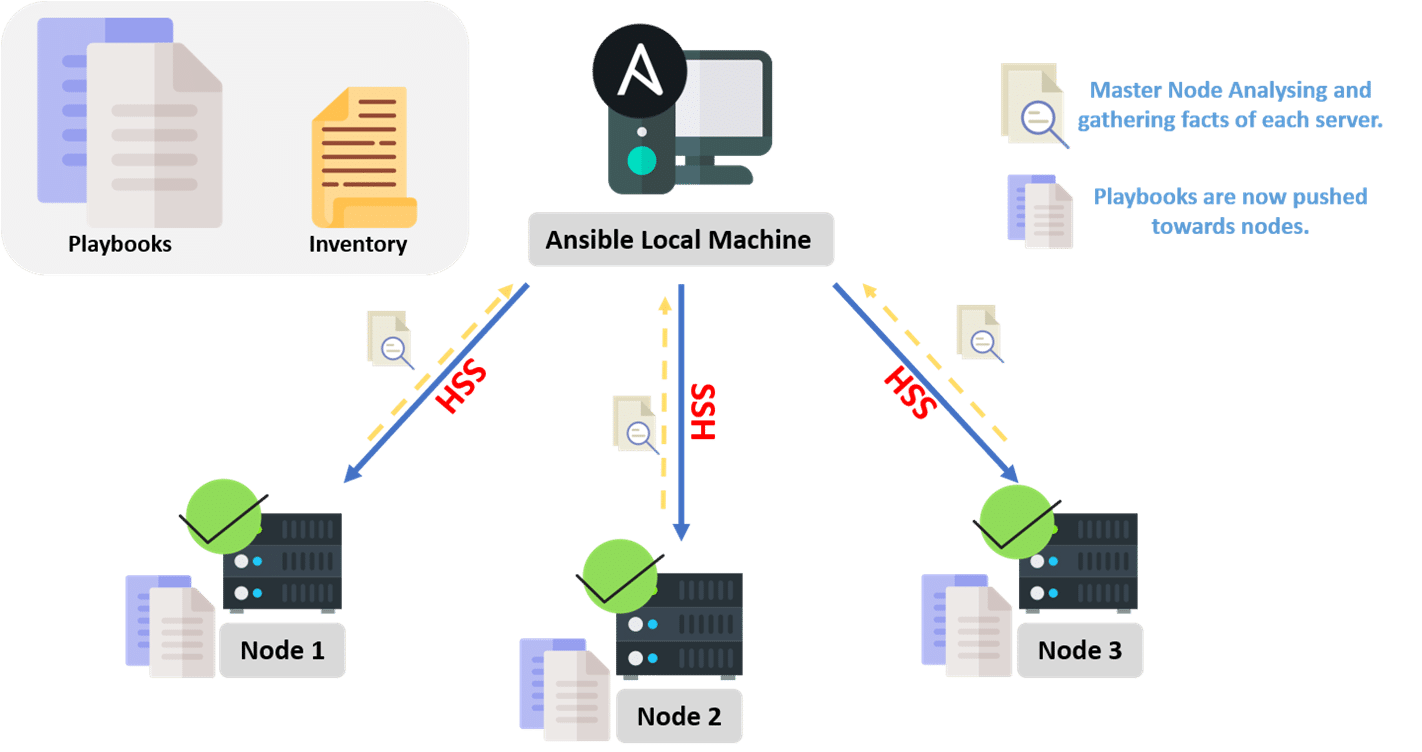
\includegraphics[width=0.9\columnwidth]{images/ansible01.PNG}
	\caption{Modelo general de funcionamiento de Ansible.}
	\label{fig:ansible01}
\end{figure}

\subsubsection{Arquitectura}
\par Al estar diseñado para despliegues de varios niveles, Ansible modela la infraestructura de TI al describir cómo todos los sistemas se interrelacionan, en lugar de solo administrar un sistema a la vez. En la Figura \ref{fig:ansible02} se presenta una arquitectura con máquinas host que se conecta a un servidor ansible y envía los Playbooks a través de SSH como Muestra la Figura \ref{fig:ansible01}.\\

\begin{figure}[htpb!]
	\centering
	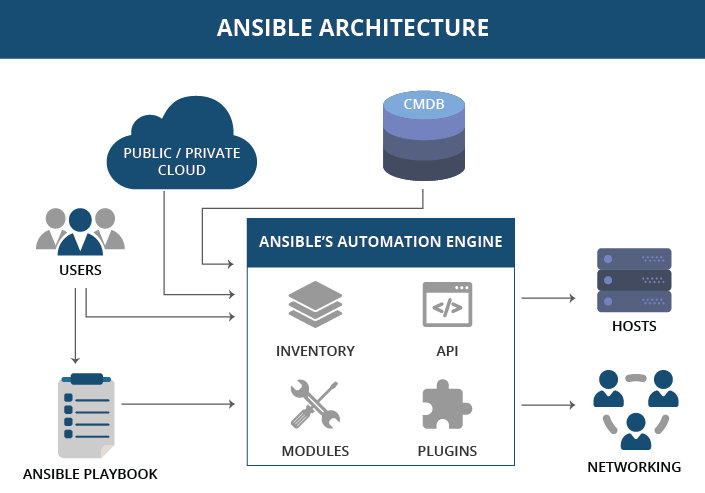
\includegraphics[width=0.8\columnwidth]{images/ansible02.PNG}
	\caption{Arquitectura de Ansible.}
	\label{fig:ansible02}
\end{figure}
\par A continuación, se explican algunos de los componentes del funcionamiento de Ansible \cite{BOOK13}:\\

\textbf{\textit{Playbooks}:} Los libros de jugadas o playbooks, son el lenguaje mediante el cual Ansible organiza, configura, administra y despliega sistemas. Los libros de jugadas definen el flujo de trabajo de las tareas en los hosts, ellos son muy simples de escribir, ya que es código YAML. El código YAML es un lenguaje de serialización de datos.\\

\textbf{\textit{Inventory}:} Un Inventario o inventory, es un archivo que describe Hosts y Grupos en Ansible. El inventario también se puede proporcionar a través de un Script de inventario, que es un programa que busca hosts, miembros de grupos para hosts e información variable de un recurso externo, ya sea una base de datos SQL o una solución CMDB.\\

\textbf{\textit{Host}:} Un host es simplemente una máquina remota que Ansible gestiona. Pueden tener variables individuales asignadas a ellos y también pueden organizarse en grupos. Todos los hosts tienen un nombre al que se puede acceder (que es una dirección IP o un nombre de dominio) y, opcionalmente, un número de puerto si no se puede acceder en el puerto SSH predeterminado.\\

\textbf{Grupo:} Un grupo consta de varios hosts asignados que pueden dirigirse juntos, así como variables dadas que comparten en común.\\

\textbf{Roles:} Los roles son unidades de organización en Ansible. Asignar un rol a un grupo de hosts (o un conjunto de grupos, o patrones de host, etc.), implica que ellos deben implementar un comportamiento específico. Un rol puede incluir la aplicación de uno o mas valores variables, tareas y controladores.\\

\textbf{\textit{Public/Private Cloud}:} La nube (publica, privada o híbrida) es el servidor. También puede actuar como repositorio para todas las configuraciones y la instalación de TI.\\

\textbf{\textit{Modules}:} Ansible funciona conectándose a sus nodos y enviando scripts llamados Ansible modules a ellos. La mayoría de los módulos aceptan parámetros que describen el estado deseado del sistema. Ansible luego ejecuta estos módulos (sobre SSH por defecto) y los elimina cuando finaliza. Su biblioteca de módulos puede residir en cualquier máquina y no se requieren servidores, demonios o bases de datos.\\

\textbf{\textit{Plugins}:} Los complementos o plugins, son un tipo especial de módulos, ellos se ejecutan en la máquina de control principal para fines de registro. Hay complementos de devolución de llamada que permiten conectarse a diferentes eventos ansibles para fines de visualización y registro. Los complementos de caché se utilizan para mantener un caché de hechos para evitar costosas operaciones de recopilación de datos. Ansible también tiene complementos de acción, que son módulos de ``front-end'' y pueden ejecutar tareas en la máquina controladora antes de llamar a los propios módulos.\\

\par En la red, Ansible hace uso de SSH para comunicarse con los distintos host. También se puede hacer uso de una API en Python para controlar nodos y responder a eventos de Python.

\subsubsection{Ansible Tower}

\par Ansible Tower es una interfaz basada en web para administrar Ansible. Una de las necesidades principales que requerian los usuarios de Ansible, era una interfaz fácil y rápida para administrar despliegues y monitorear las configuraciones. Para resolver esto, la administración de Ansible  presentó  Ansible Tower. Algunas de las características importantes de Ansible Tower se enumeran a continuación:
\begin{itemize}
    \item Control de acceso basado en roles: puede configurar equipos y usuarios en varios roles.
    \item Programación de trabajos: programa trabajos y establece opciones de repetición.
    \item Modo portal: esta es una vista simplificada de los trabajos de automatización.
    \item Tower Dashboard: permite ver la información resumida de todo el ambiente de despliegue.
    \item Integración en la nube: Tower es compatible con los principales entornos de nube.
    \item API REST completamente documentada.
\end{itemize}


%%%%%%%%%%%%%%%%%%%%%%%%
\subsection{Puppet}

\par Puppet es una herramienta de gestión de configuración de software de código abierto. Se ejecuta en muchos sistemas tipo Unix, así como en Microsoft Windows e incluye su propio lenguaje declarativo para describir la configuración del sistema. Puppet está basado en Ruby, con licencia GPLv2 y puede ejecutarse en el servidor del cliente o en modos independientes \cite{BOOK15}. Puppet se utiliza a menudo para administrar un host a lo largo de su ciclo de vida, desde su construcción e instalación inicial, durante sus actualizaciones y mantenimiento, hasta el final de su vida útil, cuando traslada servicios a otro lugar.
Puppet tiene un modelo operativo simple que es fácil de entender y desplegar. El modelo está compuesto por tres componentes: %\cite{BOOK15}:
\begin{itemize}
    \item Despliegue.
    \item Lenguaje de configuración y capa de abstracción de recursos.
    \item Capa transaccional.
\end{itemize}

\par Puppet generalmente se despliega en un modelo de servidor cliente. %(Figura \ref{fig:puppet01}). 
El servidor se llama Puppet master, el software del cliente Puppet se llama agente y el propio host se define como un nodo. Puppet master se ejecuta como un daemon en un host y contiene la configuración requerida para su entorno. Los agentes de Puppet se conectan al Puppet master a través de una conexión encriptada y autenticada usando SSL estándar y recuperan o extraen cualquier configuración que se aplique \cite{BOOK15}.\\
 
\par Puppet funciona utilizando un modo de extracción (o \textbf{pull}), donde los agentes sondean al Puppet master a intervalos regulares para recuperar configuraciones específicas del sitio y del nodo. En esta infraestructura, los nodos gestionados ejecutan la aplicación del agente Puppet, generalmente como un servicio en segundo plano.\\


\subsection{Chef}
\par Chef es otra herramienta de configuración open source, escrita en su mayoría en el lenguaje de programación Ruby. Chef es uno de los mayores sistemas de manejo de configuración usado en Linux, tambien es uno de las mas notables infraestructuras como código, es decir, administrar recursos a través del uso de scripts y código en vez configurar físicamente el hardware. Chef fue construido basándose en concepto de la computación en la nube, para permitir al usuario asignar y desasignar los recursos de la nube conforme a la demanda por el alto uso e incremento en el trafico \cite{BOOK16}.\\
\vspace{\baselineskip}

\par Chef puede ser desplegado en una arquitectura cliente servidor, mientras Chef este en modo cliente servidor, el cliente envia en mensajes cada atributo necesario del nodo al servidor, el cual hace uso de un motor de búsqueda para indexar dichos atributos y provee una API para que puedan ser consultados por los clientes, y así iniciar el proceso de configuración configuración.\\

\par El usuario escribe scripts llamados Recetas para manejar las aplicaciones, utilidades y como deben ser configurados los nodos, es decir, todas las acciones que deban ser automatizadas. Estas recetas pueden ser agrupadas para formar un libro de cocina (\textit{Cookbook}), el cual sirve  para describir el estado particular de los recursos (paquetes, servicios y archivos), Chef verifica el estado de estos y corrige si alguno no se encuentra en el estado deseado. Para realizar esta funciones Chef tiene 3 mayores componentes \cite{BOOK16}:
\begin{itemize}
    \item Chef Workstation: donde se envían los Cookbook al servidor.
    \item Chef Server: se encarga de servir de repositorio para todos los nodos.
    \item Chef Node: se comunica con el servidor para solicitar la información necesaria para realizar sus acciones de configuración sobre sus recursos.
\end{itemize}

\par Las caracteristicas de Chef permiten que sea escalable y su orientación para ser deplegado en la nube hacen que esta sea una opción popular para la automatización del proceso de configuración.

\subsection{Comparación entre Herramientas de Configuración}
\par Aunque en la actualidad existe un mucho mayor numero de herramientas de configuración, las 3 que fueron mencionadas  con anterioridad se encuentran entre las m\'as populares. Estas herramientas comparten un propósito similar, pero cabe destacar que difieren en su despliegue, por lo que presentan características distintas que se adaptan mejor a algunos casos de uso que a otros. A continuacion, se presenta una comparación entre las características de Ansible, Puppet y Chef \cite{BOOK13,BOOK15,BOOK16}:
\begin{enumerate}
    \item Lenguajes y Sintaxis: Como lenguajes de configuración Puppet y Chef se basan en Ruby, tambien en otros lenguajes propios como Puppet DSL, mientras que Ansible permite varios lenguajes como Python y Yaml, los cuales son mas utilizados en la actualidad y mas simples de comprender.
    \item Arquitectura e instalación: Puppet y Chef requieren de agentes instalados en los nodos y un servidor maestro del cual se obtienen los parámetros de configuración, lo cual es mas complejo que los requerimientos de Ansible, el cual usa una arquitectura sin agentes (no es necesario tener instalado Ansible en los nodos a configurar) y solo necesita una instalación, la cual se encarga de distribuir los Playbook.
    \item Tipo de configuración: Hay dos tipos de configuraciones, Pull y Push. La configuración de Pull implica que los nodos extraen su configuración solicitando los parámetros  a un servidor central, como funcionan Puppet y Chef. Mientras que, en una Push, todas las configuraciones de los nodos se enviarán a estos con comandos desde un equipo, este tipo de configuración es utilizado por Ansible.
    \item Escalabilidad y capacidades:  En términos de escalabilidad e interoperabilidad, las tres herramientas tienen características similares. En cuanto a sus capacidades, Chef permite la configuración de infraestructuras, Puppet tiene la posibilidad  de emitir gráficos que proporciona la visualización de todo lo que administra. Ansible permite una simple configuración e integración, con lo que permite considerarla como la herramienta mas adaptable entre las 3.
    \item Modelo: en la gestión de la configuración por software existen 2 modelos principales en los que se basan las herramientas de configuración, el modelo Declarativo y el Imperativo. En el modelo declarativo, el administrador describe el estado final deseado de la infraestructura y la herramienta intenta alcanzar dicho estado. En el imperativo, los usuarios definen comandos y el orden en que estos son ejecutados para realizar la configuración. Entre las herramientas declarativas se encuentra Puppet, mientras que Ansible (con los Playbooks) y Chef (con los Cookbooks) son herramientas que se basan en el modelo imperativo, aunque estas dos ultimas pueden llegar a utilizarse de manera declarativa también.
\end{enumerate}

\par Al comparar estas herramientas, se observan lo beneficios de una sobre las otras  y se justifica el uso de una de estas (en el cap\'itulo 4).

\section{Herramientas para la Experimentación}

\par En cuanto a las herramientas adicionales utilizadas en el proceso de experimentación necesarias para alcanzar los objetivos propuestos en capitulo 4 de este trabajo, fueron seleccionadas las siguientes:\\

\subsection{Nginx}

\par Nginx es un servidor web que también se puede utilizar como un servidor proxy para correo electrónico (IMAP, POP3 y SMTP), un proxy inverso y balanceador de carga para servidores HTTP, TCP y UDP. Nginx es un software gratuito y de código abierto \cite{WEB01}. La arquitectura modular impulsada por eventos de Nginx puede proporcionar un rendimiento predecible bajo cargas de trabajo elevadas. Nginx también posee las siguientes características:\\
\vspace{\baselineskip}
\begin{itemize}
    \item Capacidad para manejar muchas conexiones simultáneas.
    \item Manejo de archivos estáticos, archivos de índice e indexación automática.
    \item Proxy inverso con almacenamiento en caché.
    \item Compatible con IPv6.
    \item Servidores virtuales basados en nombre y dirección IP.
    \item Actualización HTTP / 1.1, compatibilidad con el protocolo HTTP / 2.
    \item Reescritura y redirección de URL.
    \item Arquitectura basada en módulos con soporte para módulos centrales y de terceros.
    \item Capacidad para registrar logs de accesos y de errores.
    \item Otras características incluyen la actualización del ejecutable y la configuración sin pérdida de conexiones del cliente.
\end{itemize}

\par Otro beneficio de Nginx es facil depliegue imagenes de este en contenedores de dockers o pods de Kubernetes, por esto su uso como herramienta en los experimentos.\\




		\chapter{Marco Procedimental}
\par Para realizar exitosamente un proyecto de desarrollo de software, es necesario escoger un método y establecer un plan de trabajo con el fin de organizar el flujo de las actividades, definir las metas y sus lapsos de tiempo de ejecución, en otras palabras, establecer una metodología de desarrollo que posibilite completar las tareas correspondientes eficientemente. \\
\par Una metodología de desarrollo de software puede ser definido como un conjunto estandarizado de conceptos, prácticas y criterios con la finalidad de estructurar, planear y controlar un proceso de desarrollo de software de calidad, a menudo ella es vinculada a algún tipo de organización, la cual promueve su uso y hace los refinamientos requeridos. A continuación, se procederá a explicar brevemente las metodologías mas utilizadas para el desarrollo de software.

\section{Metodologías Tradicionales}
\par Las metodologías Tradicionales refieren a la forma ``tradicional'' de desarrollar un software. Ellas se basan en seguir una serie secuencial de pasos, tales como definición de requisitos, creación de soluciones, pruebas e implementación. Estos requisitos deben ser definidos y documentados al comienzo del proyecto.\\
\par  Debido a estos requisitos y aspectos, estas metodologías tradicionales también son conocidas como metodologías ``pesadas''. Algunos profesionales encontraron frustrante esta visión centrada en el proceso del desarrollo de software y reportan dificultades aún cuando las tasas de cambio son relativamente bajas. Las metodologías pesadas tienen las siguientes características similares \cite{BOOK08}:
\begin{itemize}
    \item Enfoque predictivo: las metodologías pesadas tienden a primero planificar en detalle gran parte del proceso, consumiendo un largo periodo de tiempo. Este enfoque sigue una disciplina de ingeniería donde el desarrollo es predictivo y repetible. Se pone mucho énfasis en los diagramas, enfocándose en la necesidad del sistema y en cómo resolver las necesidades de manera eficiente.
    \item Documentación integral: el desarrollo de software tradicional, considera el documento de requisitos como la pieza clave de la documentación. Un proceso principal en las metodologías pesadas, es el largo proceso inicial de diseño, en el que se considera, que es posible reunir todos los requisitos por adelantado, antes de escribir cualquier código.
    \item Orientado a procesos: el objetivo de las metodologías pesadas es definir un proceso que funcione bien. El proceso consistirá en ciertas tareas que deben realizar los gerentes, diseñadores, programadores, testers, otros.
    \item Orientado a herramientas: las herramientas de gestión de proyectos, editores de código, compiladores y otras, se deben utilizar para completar y entregar cada tarea.
\end{itemize}

\section{Metodologías Ágiles}
\par En las metodologías tradicionales, no se toma en cuenta el factor humano en el desarrollo de software, así como tampoco se hace énfasis en los problemas y cambios que pueden surgir a lo largo del proyecto, por este motivo nace el término ``ágil'' aplicado al desarrollo de software. El objetivo principal de las metodologías ágiles, es destacar un nuevo grupo de valores y principios, que permitieran dar respuesta rápida a los problemas surgidos durante el desarrollo. \\
\par \textit{The Agile Alliance} es una organización sin fines de lucro, dedicada a promover los conceptos relacionados con el desarrollo ágil del software, su punto de partida fue el Manifiesto Ágil, un documento que resume su filosofía y plantea los siguientes principios \cite{BOOK06,BOOK07}:
\begin{itemize}
    \item   La mayor prioridad es satisfacer al cliente, mediante la temprana y continua entrega de software de calidad.
    \item	Los cambios en los requerimientos son bienvenidos, incluso en fases tardías del desarrollo.
    \item	Entregas frecuentes de software funcional, en intervalos de dos semanas a dos meses, dando preferencia a los tiempos más cortos.
    \item	Los clientes y los desarrolladores deben trabajar diariamente y en conjunto a lo largo del proyecto.
    \item	Construir proyectos alrededor de individuos motivados. Darles el ambiente y el apoyo que necesitan y confiar que realizarán el trabajo de manera correcta.
    \item	El método más eficiente y efectivo de comunicación entre los miembros del equipo de trabajo es la conversación cara a cara.
    \item	La principal métrica del progreso es que el software funcione correctamente.
    \item	Los procesos ágiles promueven un desarrollo sostenible.
    \item	Atención continua a la excelencia y el buen diseño.
    \item	La simplicidad es esencial.
    \item	Las mejores arquitecturas, requerimientos y diseños surgen de equipos de trabajo organizados por sí mismos.
    \item	El equipo analiza cómo ser más efectivo y adecua su comportamiento al resultado de discusiones realizadas regularmente. 

\end{itemize}
\subsection{Scrum}

\par Scrum es un modelo referencial, define un conjunto de prácticas, roles y el punto de partida para la creación del proceso a ejecutar según la duración del proyecto \cite{BOOK11}. \\

\par Scrum no requiere ni proporciona métodos/prácticas de desarrollo de software específicos para ser utilizados. En cambio, requiere ciertas prácticas y herramientas de gestión en diferentes fases de Scrum, para evitar el caos por impredecibilidad y complejidad.
\subsubsection{Prácticas Principales}
\begin{itemize}
    \item Backlog del Producto: es la lista priorizada de todas las características y cambios que aún deben realizarse en el sistema, requerido por múltiples actores.
    \item Sprints: Las herramientas de gerencias del equipo son las reuniones de planificación de Sprint, la revisión del Sprint y las reuniones diarias de Scrum.
    \item Reunión de planificación de Sprint.
    \item Sprint Backlog: es la lista de funciones que realmente se asigna a un Sprint en particular. 
    \item Scrum diario: es una reunión diaria de aproximadamente 15 minutos. 
\end{itemize}

\par El proceso Scrum puede cambiar considerablemente la descripción del trabajo y las costumbres del equipo del proyecto Scrum \cite{BOOK08,BOOK11}.
%%%%%%%%%%%%%%%

\subsection{XP: \textit{Extreme Programming}}

\par El proceso XP se caracteriza por ciclos cortos de desarrollo, planificación incremental, retroalimentación continua, dependencia de la comunicación y diseño evolutivo \cite{BOOK10}. Los miembros del equipo XP dedican muchas veces al día unos minutos a la programación, unos a la gestión del proyecto, otros al diseño, a la retroalimentación y al trabajo en equipo \cite{BOOK09}. A continuación se muestra un resumen de los términos y prácticas de XP \cite{BOOK09,BOOK10}:
\begin{itemize}
    \item \textbf{Planificación:} el programador estima el esfuerzo necesario para la implementación, el cliente decide el alcance y el momento de los lanzamientos en función de las estimaciones.
    \item \textbf{Lanzamientos cortos:} la aplicación se desarrolla en una serie de versiones pequeñas y frecuentemente actualizadas. Se lanzan nuevas versiones en frecuencia desde diario a mensual.
    \item \textbf{Diseño simple:} el énfasis está en el diseño de la solución más simple posible. La complejidad innecesaria y el código adicional se eliminan de inmediato.
    \item \textbf{Metáfora:} el sistema se define mediante un conjunto de metáforas entre el cliente y los programadores, que describen cómo funciona el sistema.
    \item \textbf{Refactorizar:} implica la reestructuración del sistema simplificándolo, eliminando la duplicación, mejorando la comunicación y agregando flexibilidad.
    \item \textbf{Programación en pares:} todo el código de producción lo realizan dos programadores en una computadora.
    \item \textbf{Integración continua:} todo código nuevo se integra con el sistema tan pronto como esté listo. Al integrarse, el sistema se construye nuevamente y los cambios son aceptados una vez que pasan todas las pruebas.
    \item \textbf{Cliente en el sitio:} el cliente debe estar disponible en todo momento con el equipo de desarrollo.
    \item \textbf{Estándares de codificación:} existen reglas para la escritura de todo código y los desarrolladores las siguen para brindar consistencia y mejorar la comunicación entre el equipo de desarrollo.
\end{itemize}

\par El ciclo de vida de un proyecto XP se divide en seis fases: exploración, planificación, iteraciones para el lanzamiento, producción, mantenimiento y muerte, Ver figura \ref{fig:xp01}. 

\begin{figure}[htpb!]
	\centering
	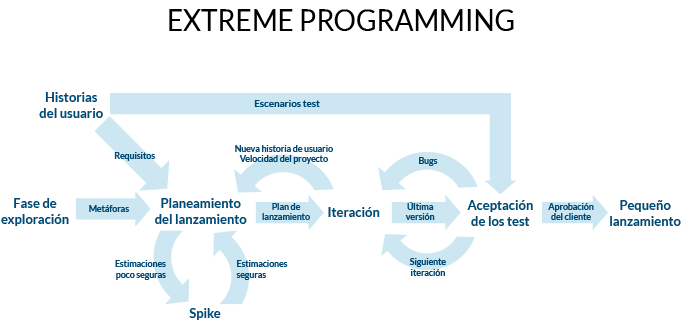
\includegraphics[width=0.91\columnwidth]{images/xp01.png}
	\caption{Ciclo de vida de XP.}
	\label{fig:xp01}
\end{figure}

\subsection{Kanban}

\par El enfoque Kanban es una de las adiciones más reciente al desarrollo de software ágil, pero fue introducida por la industria Japonesa en el año 1950. El método Kanban en el desarrollo de software se originó en 2004 y se basa en impulsar a los equipos de proyectos a visualizar el flujo de trabajo, limitar el trabajo en progreso (WIP o Work In Progress por sus siglas en ingles) en cada etapa del flujo de trabajo y medir el tiempo del ciclo \cite{LIB22}.\\ 

\par Kanban se basa en el uso de un tablero o panel llamado tabla Kanban  (Ver \ref{fig:xp01}), que  proporciona visibilidad al proceso de software, porque muestra el trabajo asignado a cada desarrollador, comunica claramente las prioridades y destaca los cuellos de botella. Además, su objetivo es minimizar el WIP, es decir, desarrollar solo los elementos que se solicitan. Esto produce un flujo constante de elementos de trabajo liberados a los clientes, ya que los desarrolladores se centran solo en esos pocos elementos en un momento dado. El método Kanban tiene como objetivo adaptar rápidamente el proceso mediante el uso de ciclos de retroalimentación más cortos \cite{LIB22}.\\

\par Los siguientes son los principios básicos de Kanban, los cuales son necesarios resaltados en el tablero, para el desarrollo de software son \cite{LIB23}:
\begin{itemize}
    \item Limitación del trabajo en proceso (WIP).
    \item Tirando valor a través del proceso de desarrollo.
    \item Hacer visible el proceso de desarrollo.
    \item Aumento del rendimiento.
    \item Utilizando un listado de tareas fijo (tablero).
    \item Calidad de acoplamiento.
\end{itemize}

\begin{figure}[htpb!]
	\centering
	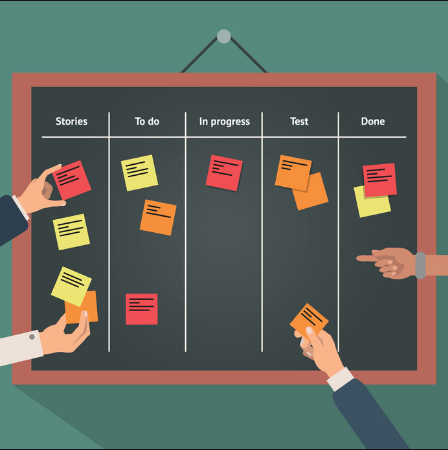
\includegraphics[width=0.875\columnwidth]{images/kanban01.PNG}
	\caption{Tablero Kanban.}
	\label{fig:kanban01}
\end{figure}

\par La metodología Kanban se enfoca en hacer el trabajo correcto en el momento adecuado, dados los conjuntos de habilidades de los desarrolladores y velocidades de trabajo. Estos comienzan implementando componentes del proyecto que agregan valor al proyecto. También se evita implementar funciones innecesarias, escribir más especificaciones de las que puedan codificar y  código del que pueda probar, para no probar mas código del que se pueda implementar. Por esto Kanban elimina cualquier desperdicio en cada paso \cite{LIB23}.

		\chapter{Marco Aplicativo}

\par En la investigación presentada se destaco la importancia de realizar pruebas de los sistemas de computo antes, durante y después de su desarrollo, los beneficios y dificultades que conlleva el despliegue de una nube híbrida, así como la relevancia de la inyección de fallas y la tendencia actual de este tipo de actividades de pruebas, debido a su importancia en los sistemas para mejorar el comportamiento de estos en caso de fallas.\\\\\\\\\\\\\\\\\\\\\\\\\\\\\\\\\\\\\\\\\\\\\\\\\\\\\\\\\\\\\\\\\\\\\\\\
\par Se planteo el desarrollo de un sistema automatizado con herramientas previamente definidas y comparadas, para obtener un entorno de pruebas e inyectar fallas a un clúster de Kubernetes, posteriormente con la respuesta obtenida podremos comparar el comportamiento del clúster al sufrir la falla con un estado óptimo previamente capturado, y establecer la respuesta del sistema a la falla tratada. Se utilizo Ansible para la automatización de las pruebas y así el usuario que utilice el sistema pueda escoger de manera controlada las fallas que desea inyectar. Con la ayuda de Minikube se desplegó un clúster de Kubernetes con un único nodo. Se despliega el clúster de Kurbenetes haciendo uso del container runtime Dockers para el despliegue de los Pods. El uso de estas herramientas sobre otras de similar propósito es respaldado por el hecho que son ampliamente utilizadas, son open source, existe el fácil acceso a la documentación y se posee conocimiento previo en el uso de estas.\\
%%%%%%%%%%%
\section{Objetivos}\label{sec:41}
\par Para el trabajo especial de grado se presentaron los siguientes objetivos:

%%%%%%%%%%%
\subsection{Objetivo General}


\par Estudiar la respuesta de un cluster de Kubernetes a fallas controladas en recursos de red, procesamiento y almacenamiento.

%%%%%%%%%%%
\subsection{Objetivos Específicos}
\begin{itemize}    
    \item Implementar un entorno básico que permita la ejecución de pruebas de inyección de fallas en un cluster de Kubernetes basadas en colecciones y roles de Ansible.
    \item Diseñar pruebas de inyección de fallas para causar interrupciones de servicio en un cluster de Kubernetes.
    \item Aplicar pruebas de inyección de fallas basadas en colecciones de Ansible para:
    \begin{itemize}
        \item Simular sobrecarga de CPU.
        \item Simular saturación de disco. 
        \item Introducir sobrecarga en las interfaces de red.
        \item Introducir latencia en la comunicación entre aplicaciones.
    \end{itemize}
    \item Caracterizar el comportamiento del cluster de Kubernetes en respuesta a la inyección de las fallas consideradas.
    \item Generar los resultados de las pruebas de inyección de fallas:
    \begin{itemize}
        \item Determinar si el sistema es capaz de recuperarse.
        \item Evaluar el posible tiempo de recuperación.
        \item Identificar, cuantificar y recolectar datos en caso de perdida de paquetes.
    \end{itemize}
\end{itemize}
%%%%%%%%%%%
\section{Metodología para el Desarrollo}


\par Las metodologías ágiles son ampliamente utilizadas en las operaciones de desarrollo por muchas organizaciones en la actualidad, su utilidad puede ser aplicada a la implementación de pruebas de inyección de fallas.\\ %\cite{LIB03}
\par En este se selecciono y aplico una metodología de desarrollo ágil, con las respectivas modificaciones que se mencionan posteriormente, con el fin de fomentar el proyecto. De las metodologías ágiles se selecciono Kanban, ya que ella fue la que mejor se adapto a los requerimientos de los experimentos de inyección de fallas a realizados. Su similar simplicidad con XP y uso en la actualidad en el desarrollo de software justifica el uso de Kanban, a su vez la carencia de tener que rellenar roles específicos y realizar eventos, lo ubica por encima sobre Scrum para su uso en el proyecto. La metodología Kanban, tiene principio y características  que justifican su utilización en el proyecto, entre los que destacan:
\begin{itemize}
    \item Flexibilidad en su aplicación: como marco de trabajo, Kanban es flexible y solo deben seguirse sus lineamientos y principios, en ningún caso limita las herramientas que se pueden utilizar, brindando notable independencia en el trabajo al equipo.
    \item Simplicidad: entre los mayores beneficios que tiene Kanban es su simplicidad, ya que contiene relativamente pocos roles a llenar y sólo requiere que se implementen unos pocos artefactos para almacenar la información necesaria y atender algunos eventos.
    \item Amplia flexibilidad a los cambios: Kanban acepta la posibilidad de modificaciones simples en su proceso y en las prioridades de desarrollo de éstos durante alguna iteración.
    \item Eficiencia: Kanban permite al equipo auto-organizarse y al integrar un diseño simple, permite incrementar la eficiencia del equipo de trabajo.
    \item Trabajo en equipo: el trabajo en equipo es aceptado en el método Kanban, que permite que exista una retroalimentación, mejorando la comunicación y optimizando el uso del tiempo.
\end{itemize} 
\par El marco de trabajo Kanban requirió de la siguiente modificación para adaptarse a las necesidades del proyecto:
\begin{itemize}
    \item Documentación y análisis de resultados: aunque muchos procesos ágiles como Kanban contemplan la documentación del trabajo mediante ciertos artefactos, ellos no inducen la recopilación de información de manera exhaustiva. Para poder adaptar este marco a nuestras necesidades de conveniente gestión del conocimiento, es necesario reunir y documentar toda la información posible en cada una de las etapas, analizar los resultados y compararlos con estados estables y/o anteriores. 
\end{itemize}
 
%%%%%%%%%%%
\section{Alcance}


\par En la actualidad, las organizaciones, sin importar su tamaño, requieren probar la fiabilidad de su entorno de cómputo híbrido en sus operaciones de desarrollo, para asegurar un servicio estable y confiable. Este proyecto propone estudiar la respuesta de un cluster de Kubernetes a fallas controladas en recursos de red, procesamiento y almacenamiento. Especificamente se consider\'o la inyecci\'on de las siguientes fallas: i) estr\'es por CPU; ii) estr\'es por latencia; iii) estr\'es por memoria RAM y iv) estr\'es por disco; y se evaluo el efecto de cada una de ellas por separado en un entorno de Kuberenetes con deployments de dos replicas. Estas son las fallas que comunmente pueden afectar la calidad de servicio en sistemas desplegados en una red, o mas a\'un, en la internet, donde m\'ultiples usuarios intentan acceder a un recurso, aumentando la carga del sistema, y as\'i el uso de los recursos. Se realiza con dos replicas para estudiar el comportamiento de Kubernetes en el caso de poseer un pod ``sano'' y uno ``enfermo'' y en el caso de que ambas replicas se encuentran afectadas. \\ %(insertar justificacion de pq esas fallas y porque dos replicas nada mas). \\  

\par El estudio está dirigido a aquellas organizaciones que deseen implementar experimentos de inyección de fallas en la nube híbrida, utilizando herramientas que pueden ser obtenidas con facilidad y a su vez probar la capacidad de sus servicios, en caso de eventos indeseables a lo largo de su desarrollo. \\

% \par A su vez en el estudio se plantearan ciertas incógnitas sobre como se comporta Kubernetes ante ciertas fallas y se buscara responderlas.

%%%%%%%%%%%
\section{Arquitectura Propuesta}

\par El usuario ejecutara módulos de Ansible, lo cual
desencadenara la ejecución de un código de python en el nodo maestro de Kubernetes y así se inyectaran las fallas, apoyándonos con la API server de Kubernetes para acceder a todo el clúster. En la figura \ref{fig:arq02} se presenta la arquitectura básica propuesta.
\begin{figure}[htpb!]
	\centering
	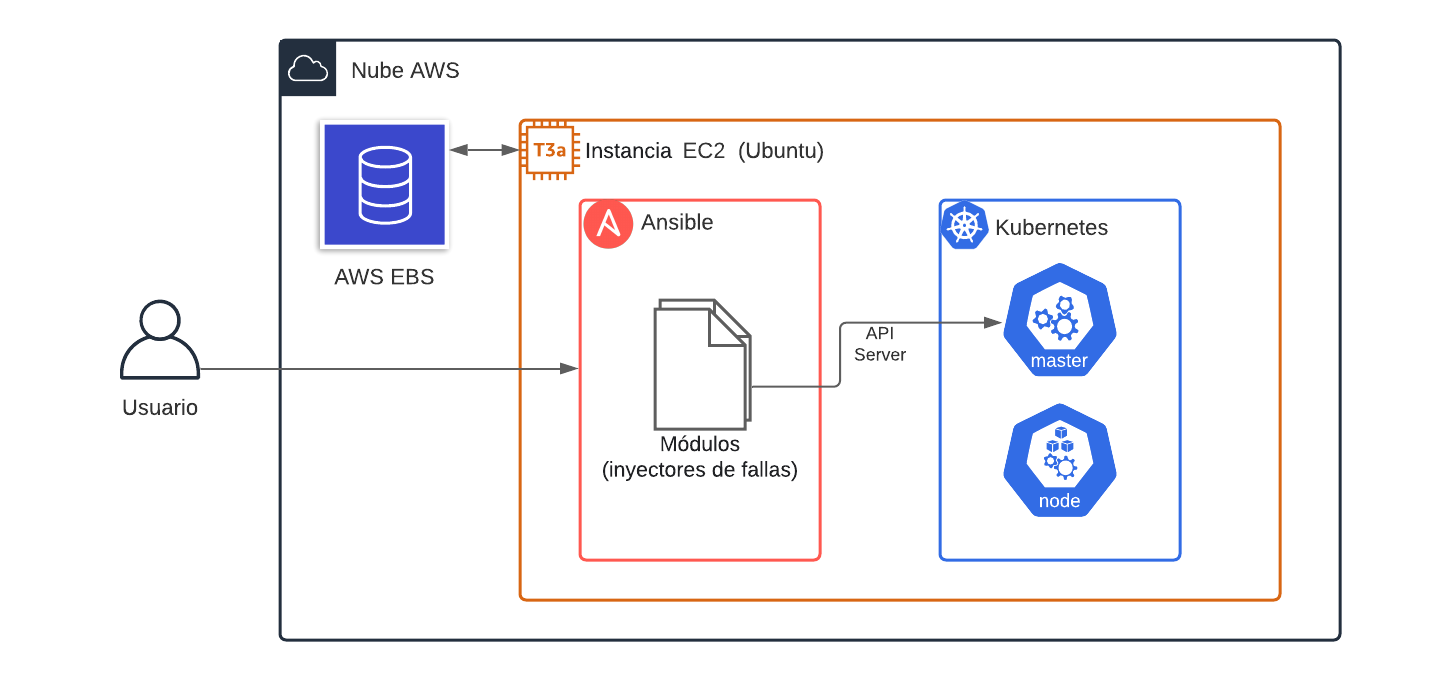
\includegraphics[width=0.95\columnwidth]{images/arq02.png}
	\caption{Arquitectura de la propuesta para el trabajo de grado.}
	\label{fig:arq02}
\end{figure}

\par Para la implementación anterior se plantea el uso de maquinas virtuales (VM), creando %2 instancias
una (1) instancia EC2 de AWS (Amazon Web Services) debido a que se posee conocimientos sobre este servicio y es de fácil acceso. La m\'aquina se configura con las siguientes características:

\begin{itemize}
    \item Para la instalación de Kubernetes de un solo nodo (Minikube) se configura una EC2 t3a.medium de AWS, con 2 vCPUs AMD EPYC 7000 de 2.5 GHz, 4GB de memoria RAM y sistema operativo Linux Ubuntu 20.04, a su vez se configura un AWS EBS de 8GB SSD para que funcione como la memoria en disco de dicha EC2.
\end{itemize}

\par A su vez fue necesaria la implementación de un ambiente local, en un equipo con capacidades de 32Gb de RAM, CPU de 4 núcleos y disco HDD. Fue configurada una maquina virtual para implementar un ambiente similar a la instancia de pruebas creada en AWS, la cual tiene las siguientes características:
\begin{itemize}
    \item La configuración cuenta también con la instalación de Kubernetes de un solo nodo (Minikube), la VM cuenta con dos 2 núcleos de CPU, a su vez cuenta con 4GB de memoria RAM, sistema operativo Linux Ubuntu 20.04 server, el adaptado de red fue configurado en modo puente (bridge) y cuenta con un almacenamiento de 20GB de disco virtual.
\end{itemize}
%%%%%%%%%%%

\section{Desarrollo de un sistema de inyecci\'on de fallas dirigido a Kubernetes}

\par Para la implementación del entorno y de los test de inyección de fallas, fue necesario realizar las actividades que se expondrán a continuación, que a su vez fueron divididas en subtareas, conforme a lo requerido al marco metodológico Kanban para poder diseñar y desarrollar dichos test. Algunas macro actividades derivan de los objetivos propuestos anteriormente en este capitulo y consistieron en:

\subsection{Implementación y despliegue del entorno de pruebas}

\par Para la implementación y despliegue del entorno de pruebas, propuesto en la arquitectura señalada anteriormente en este cap\'itulo, fue necesario el desarrollo de las tareas que se describen a continuación:\\

\subsubsection{Configuración de maquinas}
\par En lo que se refiere a la configuración de las maquinas necesarias para el desarrollo de este trabajo de investigación, se realizo la configuración de las maquinas expuestas con anterioridad en la sección 4.4 de este cap\'itulo, las cuales comparten características similares respecto a:
\begin{itemize}
    \item La instancia de AWS posee 2 vCPU y la instancia local tiene 2 núcleos de cpu, de 4 que posee el hardware.
    \item Ambas instancias poseen 4GB de memoria Ram configurada.
    \item Fue instalado el sistema operativo Linux Ubuntu 20.04 LTS para sevidores en ambas instancias (El sistema operativo fue seleccionado debido a que era una de las versiones mas actuales al momento de iniciar la investigación, siendo Ubuntu una de las distribuciones mas populares y usadas de Linux). 
\end{itemize}
\par Fue necesario el uso de un hypervisor (capa de software para realizar una virtualización de hardware) para configurar la m\'aquina virtual local. Se utilizo Vmware Workstation 15 Player como el hypervisor de preferencia, aunque otro hypervisor que permita el mismo nivel de configuración y personalizaci\'on de máquinas virtuales puede ser utilizado (como VirtualBox de Oracle), el Workstation 15 Player fue seleccionado solo porque  ya se posee conocimiento previo de esta herramienta.\\

\par Para disco, la m\'aquina local posee 20GB de disco virtual sobre un disco duro HDD, a diferencia de la instancia de AWS que solo se le configuro un EBS de 8GB de SSD.\\

\par En el ambiente local fue necesario la configuración del adaptador de red en modo Bridge para poder asignar a la maquina una dirección ip dentro de una red local para las pruebas, lo que permitió el fácil acceso al equipo a través de SSH, para la ejecución de comandos en esta maquina. El resumen de la configuración de la m\'aquina virtual local se puede observar en la imagen \ref{fig:vm01}, todos los demás aspectos de la configuración del hardware se aceptaron por defecto  de la herramienta de virtualizaci\'on.

\begin{figure}[htpb!]
	\centering
	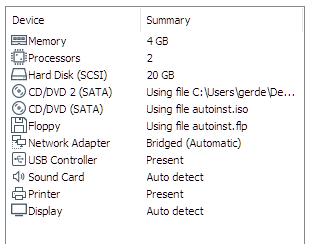
\includegraphics[width=0.70\columnwidth]{images/vm01.PNG}
	\caption{Arquitectura de la propuesta para el trabajo de grado.}
	\label{fig:vm01}
\end{figure}

\subsubsection{Instalación de herramientas: Minikube}

\par Las maquinas previamente mencionadas fueron configuradas con los requerimientos mínimos necesarios para la instalación de Minikube (Kubernetes de un solo nodo), también es necesario un container runtime como Docker (o similarmente compatible) o un entorno de máquina virtual. Para la instalación de Minikube se realizaron los siguientes pasos (todos los comandos son para el sistema operativo Linux Ubuntu 20.04 LTS server, para otros sistemas usar el comando de función similar):
\begin{enumerate}
    \item Se instala el container runtime (en este caso Docker), para este despliegue se realizo lo siguiente:
    \begin{itemize}
        \item Se actualiza la lista de paquetes existentes, usando el manejador de paquetes apt de Ubuntu:\begin{itemize}
            \item \textbf{sudo apt update}
        \end{itemize}
        \item Se instala algunos paquetes de requisitos previos que permitan a apt usar paquetes a través de HTTPS:
        \begin{itemize}
            \item \textbf{sudo apt install apt-transport-https ca-certificates curl software-properties-common}
        \end{itemize}
        \item Se añade la clave de GPG para el repositorio oficial de Docker en su sistema, tranferimos la llave desde curl que es una herramienta para tranferir data desde un servidor o a un servidor (con las banderas -fsSL, f para que en caso de falla no proporcione la salida, s para que no proporcione ningún mensaje del progreso, S solo despliegue un mensaje de error y L para seguir a la nueva ubicación en caso de que esta haya cambiado):
        \begin{itemize}
            \item \textbf{curl -fsSL https://download.docker.com/linux/ubuntu/gpg | sudo apt-key add -}
        \end{itemize}
        \item Se agrega el repositorio de Docker a las fuentes de apt:
        \begin{itemize}
            \item \textbf{sudo add-apt-repository ``deb [arch=amd64]\\ https://download.docker.com/linux/ubuntu focal stable''}
        \end{itemize}
        \item Se actualiza la lista de paquetes de nuevo con el repositorio de Docker agregado:
        \begin{itemize}
            \item \textbf{sudo apt update}
        \end{itemize}
        \item Se verifica que Docker se va a instalar desde el repositorio agregado con el comando:
        \begin{itemize}
            \item \textbf{apt-cache policy docker-ce}
        \end{itemize}
        \item Y se procede a instalar Docker con apt:
        \begin{itemize}
            \item \textbf{sudo apt install docker-ce}
        \end{itemize}
        \item Si se desea se puede verificar que Docker se instalo y esta en funcionamiento con:
        \begin{itemize}
            \item \textbf{sudo systemctl status docker}
        \end{itemize}
    \end{itemize}
    \item Antes de instalar Minikube, se instala el cliente de Kubernetes o kubectl a continuación:
    \begin{itemize}
        \item Se actualiza el repositorio apt:
        \begin{itemize}
            \item \textbf{sudo apt-get update}
        \end{itemize}
        \item Y se instalan los paquetes necesarios para usar el repositorio de Kubernetes en apt:
        \begin{itemize}
            \item \textbf{sudo apt-get install -y apt-transport-https ca-certificates curl}
        \end{itemize}
        \item Se descarga la llave de Google Cloud con curl:
        \begin{itemize}
            \item \textbf{sudo curl -fsSLo /usr/share/keyrings/kubernetes-archive-keyring.gpg \\https://packages.cloud.google.com/apt/doc/apt-key.gpg}
        \end{itemize}
        \item Luego se añade el repositorio de Kubernetes a apt:
        \begin{itemize}
            \item \textbf{echo ``deb[signed-by=/usr/share/keyrings/kubernetes-archive-keyring.gpg]\\ https://apt.kubernetes.io/ kubernetes-xenial main'' | sudo tee\\ /etc/apt/sources.list.d/kubernetes.list}
        \end{itemize}
        \item Se vuelve a actualizar apt:
        \begin{itemize}
            \item \textbf{sudo apt-get update}
        \end{itemize}
        \item Para instalar kubectl con apt:
        \begin{itemize}
            \item \textbf{sudo apt-get install -y kubectl}
        \end{itemize}
        \item Se verifica la instalación de kubectl:
        \begin{itemize}
            \item \textbf{kubectl version --client}
        \end{itemize}
    \end{itemize}
    \item Una vez instalado Docker y kubectl, se procede a realizar la instalacion de Minikube, el cual requiere que el equipo tenga por lo menos las siguientes características:
    \begin{itemize}
        \item 2 CPUs o mas.
        \item 2GB de memoria RAM o mas.
    \end{itemize}
    \item Luego se procede a obtener la descarga binaria de Minikube haciendo uso de curl (de nuevo con la bandera L para seguir a la ubicación y la bandera O para escribir el archivo remoto obtenido en un archivo local):
    \begin{itemize}
        \item \textbf{curl -LO https://storage.googleapis.com/minikube/releases/latest/minikube-linux-amd64}
    \end{itemize}
    \item Se instala Minikube con el siguiente comando: 
    \begin{itemize}
        \item \textbf{sudo install minikube-linux-amd64 /usr/local/bin/minikube}
    \end{itemize}
    \item Se inicia Minikube con los siguientes comandos:
    \begin{itemize}
        \item Si no se tiene acceso root: 
        %--driver=docker se usa en el primer inicio en caso de que se requiera especificar el driver de virtualizaci\'on, y se usa Docker debido a que es uno de los driver que pueden ser utilizados sin ser root
        \begin{itemize}
            \item \textbf{minikube start --drive=docker}
        \end{itemize}
        \item En caso de querer iniciar minikube con acceso root: 
        %en este comando no se especifica driver debido a que root no lo necesita y se asigna el apiserver a localhost
        \begin{itemize}
            \item \textbf{sudo minikube start --vm-driver=none --apiserver-ips 127.0.0.1 --apiserver-name localhost}
        \end{itemize}
    \end{itemize}
\end{enumerate}
\par Al culminar de realizar todos los pasos, se obtiene un instalación de Minikube con lo necesario para el depliegue de pods.


\subsubsection{Instalación de herramientas: Ansible}

\par Para la inyección de las fallas en el ambiente de Kubernetes de un solo nodo previamente instalado siguiendo los pasos anteriores, se propuso el uso de la herramienta de configuración  Ansible. Esta herramienta fue utilizada para la inyección de fallas y aplicar las pruebas basadas en colecciones de Ansible. Para poder instalar la herramienta se realizaron los siguientes pasos:
\begin{enumerate}
    \item Se inicia actualizando apt:
    \begin{itemize}
        \item \textbf{sudo apt update}
    \end{itemize}
    \item Se instala el archivo de paquetes personal o PPA, este software proporciona una abstracción de los repositorios de apt utilizados y permite administrar fácilmente la distribución y las fuentes de software de proveedores de software independientes:
    \begin{itemize}
        \item \textbf{sudo apt install software-properties-common}
    \end{itemize}
    \item Luego se agrega el repositorio de Ansible y actualiza el PPA:
    \begin{itemize}
        \item \textbf{sudo add-apt-repository --yes --update ppa:ansible/ansible}
    \end{itemize}
    \item Finalizar instalando Ansible con el comando:
    \begin{itemize}
        \item \textbf{sudo apt install ansible}
    \end{itemize}
\end{enumerate}

\par Después de ejecutar todos estos comandos, el ambiente deberia estar configura con todas las herramientas propuestas en la arquitectura.

\subsection{Diseño de test de inyección}
\par Al haber implementado el entorno de pruebas basado en tecnologías para el despliegue de entornos en la nube, se procedió a el diseño de las pruebas de inyección de fallas necesarias para poder caracterizar y poner a pruebas el ambiente desplegado. Se tomo en consideración para la elaboración de los test, las herramientas utilizadas como Minikube (Kubernetes de un solo nodo) y Ansible, por ello el uso de lenguajes como Python y de archivos de configuración YAML, debido a que estas herramientas proveen una buena integración  a través del uso de APIs y de un DSL. En el diseño de las pruebas se realizaron las siguientes actividades para poder cumplir con lo propuesto:

\subsubsection{Elaboración de Artefactos : Diagrama y especificación de Casos de Uso}
\par Para el desarrollo de los test de inyección de fallas basadas en colecciones y roles de Ansible, sobre un cluster de Kubernetes de un solo nodo se elaboraron los artefactos de casos de uso expuestos a continuación:\\


\par \textbf{Diagrama de Casos de Uso}\\


\par En la figura \ref{fig:uc01} se muestran los casos de uso identificados para el proyecto, con sus respectivas especificaciones:
% \begin{figure}[htpb!]
% 	\centering
% 	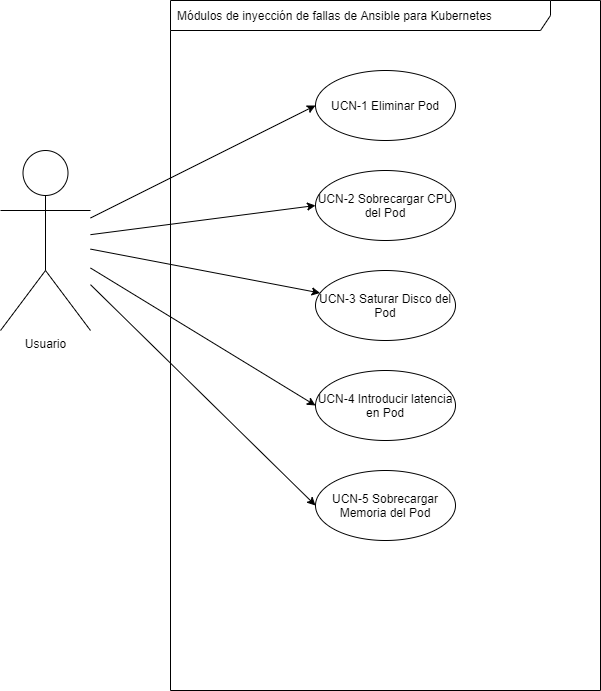
\includegraphics[width=0.70\columnwidth]{images/usecase/ucfaultinjectionfinal.png}
% 	\caption{Diagarama de Casos de Uso (UC) para los módulos de inyección de fallas en Ansible.}
% 	\label{fig:uc01}
% \end{figure}

\begin{figure}[htpb!]
	\centering
	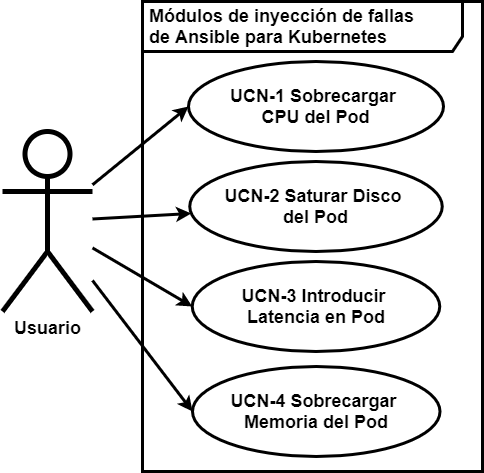
\includegraphics[width=0.43\columnwidth]{images/usecase/ucfaultinjectionF.png}
	\caption{Diagarama de Casos de Uso (UC) para los módulos de inyección de fallas en Ansible.}
	\label{fig:uc01}
\end{figure}

\textbf{Especificaciones de Casos de Uso}\\
% \par\textbf{UCN Eliminar Pod:}

% \begin{table}[htpb!]
% \tiny
% \centering
% \resizebox{\textwidth}{!}{%
% \begin{tabular}{|l|l|l|c|}
% \hline
% \rowcolor[HTML]{38FFF8}
% \textbf{UCN-1}   & \multicolumn{3}{l|}{\cellcolor[HTML]{38FFF8}\textbf{Eliminar Pod}} \\ \hline
% Dependencias     & \multicolumn{3}{l|}{Ninguna.} \\ \hline
% Precondición     & \multicolumn{3}{l|}{\begin{tabular}[c]{@{}l@{}}El usuario posee un ambiente de \\ kubernetes con un nodo de ansible \\ para ejecutar pruebas.\end{tabular}}  \\ \hline
% Descripción      & \multicolumn{3}{l|}{\begin{tabular}[c]{@{}l@{}}El módulo deberá comportarse \\ como se describe en el siguiente caso de uso \\ cuando el usuario desee eliminar uno o \\ varios Pods.\end{tabular}} \\ \hline
% Secuencia normal & Paso & \multicolumn{2}{l|}{Acción} \\ \hline & 1 & \multicolumn{2}{l|}{\begin{tabular}[c]{@{}l@{}}El usuario inicia la ejecución \\ del módulo a través de ansible \\ por consola.\end{tabular}} \\ \hline
%  & 2 & \multicolumn{2}{l|}{\begin{tabular}[c]{@{}l@{}}El usuario ejecuta el comando \\ para eliminar pods con los parámetros \\ necesarios como el namespace de pods a \\ eliminar, el nombre de un pod específico \\ a eliminar o si desea eliminar varios pods \\ aleatoriamente y la cantidad de estos.\end{tabular}} \\ \hline
%  & 3 & \multicolumn{2}{l|}{\begin{tabular}[c]{@{}l@{}}El modulo elimina el pod especifico o \\ la cantidad de pods requerida de manera \\ aleatoria, siguiendo una distribución \\ poisson por un periodo de tiempo que \\ define  $\lambda$ = 10.\end{tabular}} \\ \hline
%  & 4 & \multicolumn{2}{l|}{\begin{tabular}[c]{@{}l@{}}El sistema indica la finalización del módulo \\ sin error.\end{tabular}} \\ \hline
% Postcondición & \multicolumn{3}{l|}{\begin{tabular}[c]{@{}l@{}}El usuario observa cuales pods \\ fueron eliminados por el módulo.\end{tabular}} \\ \hline
% Excepciones & Paso & \multicolumn{2}{l|}{Acción} \\ \hline
%  & 2 & \multicolumn{2}{l|}{\begin{tabular}[c]{@{}l@{}}Si el usuario introduce algún parámetro \\ de forma errónea.\end{tabular}} \\ \hline
%   &  & E.1 & \begin{tabular}[c]{@{}l@{}}La ejecución del comando indica \\ en rojo por consola la falla del \\ parámetro erróneo.\end{tabular} \\ \hline

% \end{tabular}%
% }
% \end{table}

% \begin{table}[htpb!]
% \tiny
% \centering
% \resizebox{\textwidth}{!}{%
% \begin{tabular}{|l|l|l|c|}
% \hline
% \rowcolor[HTML]{38FFF8} 
% \textbf{UCN-1}   & \multicolumn{3}{l|}{\cellcolor[HTML]{38FFF8}\textbf{Eliminar Pod}} \\ \hline
%  &  & E.2 & El módulo finaliza su ejecución. \\ \hline
%  &  & E.3 & Se cancela el caso de uso. \\ \hline
% Comentarios & \multicolumn{3}{l|}{\begin{tabular}[c]{@{}l@{}}Los parámetros necesarios para la ejecución \\ son el nombre del namespace,  el nombre del \\ pod a eliminar o “random poisson” \\ (para eliminar aleatoriamente), la cantidad de \\ pods a eliminar (debe ser mayor o igual a 0 \\ para eliminación aleatoria e igual a 1 para un \\ pod específico) y la ubicación del intérprete \\ de python para ansible (la cual en Linux \\ por defecto es /usr/bin/python3).\end{tabular}} \\ \hline
% \end{tabular}%
% }
% \caption{Especificación de UCN1.}
% \label{tab:UCN1}
% \end{table}

\par\textbf{UCN-1 Sobrecargar CPU del Pod:}

\begin{table}[htpb!]
\tiny
\centering
\resizebox{\textwidth}{!}{%
\begin{tabular}{|l|l|l|l|}
\hline
\rowcolor[HTML]{38FFF8} 
\textbf{UCN-1} & \multicolumn{3}{l|}{\cellcolor[HTML]{38FFF8}\textbf{Sobrecargar CPU del Pod}} \\ \hline
Dependencias & \multicolumn{3}{l|}{Ninguna.} \\ \hline
Precondición & \multicolumn{3}{l|}{\begin{tabular}[c]{@{}l@{}}El usuario posee un ambiente de kubernetes con un nodo de ansible \\ para ejecutar pruebas.\end{tabular}} \\ \hline
Descripción & \multicolumn{3}{l|}{\begin{tabular}[c]{@{}l@{}}El módulo deberá comportarse como  se describe en el \\ siguiente caso de uso  cuando el usuario desee \\ sobrecargar el CPU  de uno o varios Pods.\end{tabular}} \\ \hline
Secuencia normal & Paso & \multicolumn{2}{l|}{Acción} \\ \hline
 & 1 & \multicolumn{2}{l|}{\begin{tabular}[c]{@{}l@{}}El usuario inicia la ejecución del \\ módulo a través de ansible por consola.\end{tabular}} \\ \hline
 & 2 & \multicolumn{2}{l|}{\begin{tabular}[c]{@{}l@{}}El usuario ejecuta el comando para sobrecargar \\ el CPU de un pod con los parámetros necesarios \\ como el namespace del pod, el nombre de un pod \\ específico a sobrecargar o si desea sobrecargar varios\\  pods aleatoriamente, la cantidad de estos además de \\ la duración del experimento y la dirección\\ de red del ambiente de Kubernetes.\end{tabular}} \\ \hline
  & 3 & \multicolumn{2}{l|}{\begin{tabular}[c]{@{}l@{}}El módulo sobrecarga el CPU del pod \\ seleccionado o sobrecarga el cpu de la \\ cantidad de pods requerida de manera \\ aleatoria, siguiendo una distribución poisson \\ por un periodo de tiempo que define $\lambda$  = 10.\end{tabular}} \\ \hline
 & 4 & \multicolumn{2}{l|}{Se ejecuta el módulo de inyección de forma esperada.} \\ \hline
Postcondición & \multicolumn{3}{l|}{\begin{tabular}[c]{@{}l@{}}El usuario observa cuáles pods \\ fueron sometidos al módulo de \\ sobrecarga de CPU.\end{tabular}} \\ \hline
Excepciones & Paso & \multicolumn{2}{l|}{Acción} \\ \hline
 & 2 & \multicolumn{2}{l|}{\begin{tabular}[c]{@{}l@{}}Si el usuario introduce algún \\ parámetro de forma errónea.\end{tabular}} \\ \hline
 &  & E.1 & \begin{tabular}[c]{@{}l@{}}La ejecución del comando indica por \\ consola la falla del parámetro erróneo.\end{tabular} \\ \hline
 &  & E.2 & El modulo finaliza su ejecución. \\ \hline
 &  & E.3 & Se cancela el caso de uso. \\ \hline
 Comentarios & \multicolumn{3}{l|}{{\begin{tabular}[c]{@{}l@{}}Los parámetros necesarios para la  ejecución son el nombre del \\ namespace, el nombre del pod a sobrecargar  o “random poisson” \\ (para sobrecargar pods aleatoriamente), la cantidad de pods \\ a sobrecargar (debe ser mayor o igual a 0 para sobrecarga aleatoria \\ e igual a 1 para un pod específico), la duración de ejecución del módulo \\ (experimento) y la ubicación del intérprete de python para ansible \\ (la cual en Linux por defecto es /usr/bin/python3).\end{tabular}}} \\ \hline
\end{tabular}%
}
\caption{Especificación de UCN-1.}
\label{tab:UCN1}
\end{table}



\vspace{\baselineskip}
\par\textbf{UCN-2 Saturar Disco del Pod:}

\begin{table}[htpb!]
\tiny
\centering
\resizebox{\textwidth}{!}{%
\begin{tabular}{|l|l|l|l|}
\hline
\rowcolor[HTML]{38FFF8} 
\textbf{UCN-2} & \multicolumn{3}{l|}{\cellcolor[HTML]{38FFF8}\textbf{Saturar Disco del Pod}} \\ \hline
Dependencias & \multicolumn{3}{l|}{Ninguna.} \\ \hline
Precondición & \multicolumn{3}{l|}{\begin{tabular}[c]{@{}l@{}}El usuario posee un ambiente de \\ kubernetes con un nodo de ansible \\ para ejecutar pruebas.\end{tabular}} \\ \hline
Descripción & \multicolumn{3}{l|}{\begin{tabular}[c]{@{}l@{}}El módulo deberá comportarse como se \\ describe en el siguiente caso de uso cuando \\ el usuario desee saturar el disco de uno o varios Pods.\end{tabular}} \\ \hline
Secuencia normal & Paso & \multicolumn{2}{l|}{Acción} \\ \hline
 & 1 & \multicolumn{2}{l|}{\begin{tabular}[c]{@{}l@{}}El usuario inicia la ejecución del módulo \\ a través de ansible por consola.\end{tabular}} \\ \hline
 & 2 & \multicolumn{2}{l|}{\begin{tabular}[c]{@{}l@{}}El usuario ejecuta el comando para saturar el disco \\ de un pod con los parámetros necesarios como el \\ namespace del pod, el nombre de un pod específico\\ a saturar el uso del disco o si desea saturar varios pods \\ aleatoriamente, la cantidad de estos, además de la \\ duración del experimento y la dirección\\ de red del ambiente de Kubernetes.\end{tabular}} \\ \hline
 & 3 & \multicolumn{2}{l|}{\begin{tabular}[c]{@{}l@{}}El modulo satura la memoria de disco del pod específico, \\ realizando operaciones de lectura/escritura durante el \\ periodo de tiempo.\end{tabular}} \\ \hline
 & 4 & \multicolumn{2}{l|}{Se ejecuta el módulo de inyección de forma esperada.} \\ \hline
Postcondición & \multicolumn{3}{l|}{\begin{tabular}[c]{@{}l@{}}El usuario observa el incremento en el uso \\ del disco de los pods ocasionado por el módulo \\ de saturar disco.\end{tabular}} \\ \hline
Excepciones & Paso & \multicolumn{2}{l|}{Acción} \\ \hline
 & 2 & \multicolumn{2}{l|}{\begin{tabular}[c]{@{}l@{}}Si el usuario introduce algún parámetro de \\ forma errónea.\end{tabular}} \\ \hline
 &  & E.1 & \begin{tabular}[c]{@{}l@{}}La ejecución del comando indica por consola \\ la falla del parámetro erróneo.\end{tabular} \\ \hline
 &  & E.2 & El modulo finaliza su ejecución. \\ \hline
 &  & E.3 & Se cancela el caso de uso. \\ \hline
Comentarios & \multicolumn{3}{l|}{\begin{tabular}[c]{@{}l@{}}Los parámetros necesarios para la ejecución son \\ el nombre del namespace, el nombre del pod a ser \\ sometido a la saturación de disco  o “random poisson” \\ (para saturar pods aleatoriamente), la cantidad de pods a \\ saturar (debe ser mayor o igual a 0 para saturar aleatoriamente \\ e igual a 1 para un pod específico), la duración de ejecución \\ del módulo (experimento) y la ubicación del intérprete de python \\ para ansible (la cual en Linux por defecto es /usr/bin/python3).\end{tabular}} \\ \hline
\end{tabular}%
}
\caption{Especificación de UCN-2.}
\label{tab:UCN2}
\end{table}


\vspace{\baselineskip}
\par\textbf{UCN-3 Introducir latencia en Pod:}

\begin{table}[htpb!]
\tiny
\centering
\resizebox{\textwidth}{!}{%
\begin{tabular}{|l|l|l|l|}
\hline
\rowcolor[HTML]{38FFF8} 
\textbf{UCN-3} & \multicolumn{3}{l|}{\cellcolor[HTML]{38FFF8}\textbf{Introducir Latencia en Pod}} \\ \hline
Dependencias & \multicolumn{3}{l|}{Ninguna.} \\ \hline
Precondición & \multicolumn{3}{l|}{\begin{tabular}[c]{@{}l@{}}El usuario posee un ambiente de kubernetes \\ con un nodo de ansible para ejecutar pruebas.\end{tabular}} \\ \hline
Descripción & \multicolumn{3}{l|}{\begin{tabular}[c]{@{}l@{}}El módulo deberá comportarse como se \\ describe en el siguiente caso de uso cuando \\ el usuario desee introducir latencia en una \\ aplicación de uno o varios Pods.\end{tabular}} \\ \hline
Secuencia normal & Paso & \multicolumn{2}{l|}{Acción} \\ \hline
 & 1 & \multicolumn{2}{l|}{\begin{tabular}[c]{@{}l@{}}El usuario inicia la ejecución del módulo a través de ansible \\ por consola.\end{tabular}} \\ \hline
 & 2 & \multicolumn{2}{l|}{\begin{tabular}[c]{@{}l@{}}El usuario ejecuta el comando para introducir latencia \\ en la interfaz de red de un pod con los parámetros\\  necesarios como el namespace del pod, el nombre de \\ un pod específico a ser sometido al incremento de latencia, \\ que también es introducido por el usuario, o si desea afectar \\ varios pods aleatoriamente, la cantidad de estos, además de \\ la duración del experimento y la dirección\\ de red del ambiente de Kubernetes.\end{tabular}} \\ \hline
  & 3 & \multicolumn{2}{l|}{\begin{tabular}[c]{@{}l@{}}El módulo induce latencia en la interfaz \\ de comunicación de pods través de comandos.\end{tabular}} \\ \hline
 & 4 & \multicolumn{2}{l|}{\begin{tabular}[c]{@{}l@{}}Se ejecuta el módulo de inyección de \\ forma esperada.\end{tabular}} \\ \hline
 Postcondición & \multicolumn{3}{l|}{\begin{tabular}[c]{@{}l@{}}El usuario observa la respuesta de la aplicación \\ de los pods a otras aplicaciones que fue ocasionada\\  por el módulo que introduce latencia en la interfaz \\ de red de los pods.\end{tabular}} \\ \hline
Excepciones & Paso & \multicolumn{2}{l|}{Acción} \\ \hline
 & 2 & \multicolumn{2}{l|}{\begin{tabular}[c]{@{}l@{}}Si el usuario introduce algún parámetro de \\ forma errónea.\end{tabular}} \\ \hline
 &  & E.1 & \begin{tabular}[c]{@{}l@{}}La ejecución del comando indica por consola \\ la falla del parámetro erróneo.\end{tabular} \\ \hline
 &  & E.2 & El modulo finaliza su ejecución. \\ \hline
 &  & E.3 & Se cancela el caso de uso. \\ \hline
Comentarios & \multicolumn{3}{l|}{\begin{tabular}[c]{@{}l@{}}Los parámetros necesarios para la ejecución son el \\ nombre del namespace, el nombre del pod a ser sometido \\ al incremento de latencia  o “random poisson” (para afectar \\ pods aleatoriamente), la cantidad de pods a afectar (debe ser \\ mayor o igual a 0 para afectar aleatoriamente e igual a 1 para \\ un pod específico), la duración de ejecución del módulo (experimento),  \\ la ubicación del intérprete de python para ansible (la cual en Linux por \\ defecto es /usr/bin/python3) y la “cantidad” de latencia en milisegundos.\end{tabular}} \\ \hline
\end{tabular}%
}
\caption{Especificación de UCN-3.}
\label{tab:UCN3}
\end{table}

\vspace{\baselineskip}
\par\textbf{UCN-4 Sobrecargar Memoria del Pod:}

\begin{table}[htpb!]
\tiny
\centering
\resizebox{\textwidth}{!}{%
\begin{tabular}{|l|l|l|l|}
\hline
\rowcolor[HTML]{38FFF8} 
\textbf{UCN-4} & \multicolumn{3}{l|}{\cellcolor[HTML]{38FFF8}\textbf{Sobrecargar Memoria del Pod}} \\ \hline
Dependencias & \multicolumn{3}{l|}{Ninguna.} \\ \hline
Precondición & \multicolumn{3}{l|}{\begin{tabular}[c]{@{}l@{}}El usuario posee un ambiente de \\ kubernetes con un nodo de ansible \\ para ejecutar pruebas.\end{tabular}} \\ \hline
Descripción & \multicolumn{3}{l|}{\begin{tabular}[c]{@{}l@{}}El módulo deberá comportarse como se \\ describe en el siguiente caso de uso cuando \\ el usuario desee sobrecargar la memoria de uno \\ o varios Pods.\end{tabular}} \\ \hline
Secuencia normal & Paso & \multicolumn{2}{l|}{Acción} \\ \hline
 & 1 & \multicolumn{2}{l|}{\begin{tabular}[c]{@{}l@{}}El usuario inicia la ejecución del módulo a través \\ de ansible por consola.\end{tabular}} \\ \hline
 & 2 & \multicolumn{2}{l|}{\begin{tabular}[c]{@{}l@{}}El usuario ejecuta el comando para sobrecargar la \\ memoria de un pod con los parámetros necesarios como \\ el namespace del pod, el nombre de un pod específico a \\ sobrecargar o si desea sobrecargar varios pods aleatoriamente, \\  la cantidad de estos, además de la duración del experimento\\ y la dirección de red del ambiente de Kubernetes.\end{tabular}} \\ \hline
  & 3 & \multicolumn{2}{l|}{\begin{tabular}[c]{@{}l@{}}El módulo sobrecarga la memoria del pod seleccionado \\ o sobrecarga la memoria de la cantidad de pods requerida \\ de manera aleatoria, siguiendo una distribución poisson por \\ un periodo de tiempo que define $\lambda$  = 10.\end{tabular}} \\ \hline
 & 4 & \multicolumn{2}{l|}{Se ejecuta el módulo de inyección de forma esperada.} \\ \hline
Postcondición & \multicolumn{3}{l|}{\begin{tabular}[c]{@{}l@{}}El usuario observa cuales pods fueron sometidos \\ al módulo de sobrecarga de memoria.\end{tabular}} \\ \hline
Excepciones & Paso & \multicolumn{2}{l|}{Acción} \\ \hline
 & 2 & \multicolumn{2}{l|}{Si el usuario introduce algún parámetro de forma errónea.} \\ \hline
 &  & E.1 & \begin{tabular}[c]{@{}l@{}}La ejecución del comando indica por consola la \\ falla del parámetro erróneo.\end{tabular} \\ \hline
 &  & E.2 & El modulo finaliza su ejecución. \\ \hline
 &  & E.3 & Se cancela el caso de uso. \\ \hline
Comentarios & \multicolumn{3}{l|}{\begin{tabular}[c]{@{}l@{}}Los parámetros necesarios para la ejecución son el nombre \\ del namespace, el nombre del pod a sobrecargar  o “random poisson” \\ (para sobrecargar pods aleatoriamente), la cantidad de pods a sobrecargar \\ (debe ser mayor o igual a 0 para sobrecarga aleatoria e igual a 1 para \\ un pod específico), la duración de ejecución del módulo (experimento) y \\ la ubicación del intérprete de python para ansible (la cual en Linux por \\ defecto es /usr/bin/python3).\end{tabular}} \\ \hline
\end{tabular}%
}
\caption{Especificación de UCN-4.}
\label{tab:UCN4}
\end{table}



\subsection{Desarrollo de test de inyección}

\subsubsection{Integraci\'on de la herramienta Pystol}
\par Pystol es una herramienta open source creada para demostrar la correlación entre la ejecución de una acción de inyección de fallas y el cambio en el comportamiento del clúster basado en Kubernetes. Se us\'o como base los test de esta herramienta tenia implementados, para el diseño y desarrollo de los test de este trabajo especial. Las pruebas de inyecci\'on de fallas desarrolladas puedan ser intregradas usando Ansible, tambien esta pruebas fueron desarrolladas como contribucion al proyecto opensource de la plataforma Pystol y se espera que en un futuro puedan ser integradas a esta.\\

\par Es necesario ejecutar el siguiente script para Linux (ver Figura \ref{fig:initsh}), a fin de instalar la colecci\'on de los test de inyecci\'on de fallas en Ansible, que se presentan mas adelante en este documento:

\begin{figure}[htpb!]
	\centering
	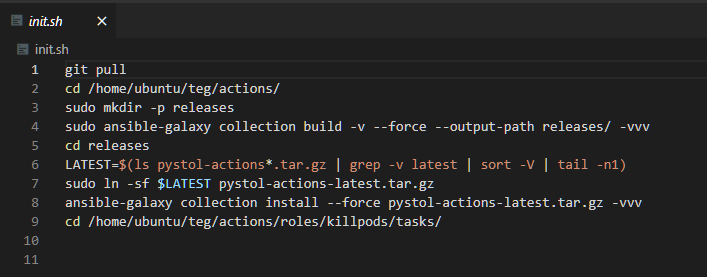
\includegraphics[width=0.95\columnwidth]{images/captures/initsh.PNG}
	\caption{Captura del Script init.sh.}
	\label{fig:initsh}
\end{figure}

\carlos{Al inyectar los fallos debe haber una herramienta  que este generando las peticiones WEB, lectura/escritura, o inyectar trafico. Que herramienta estan utilizando, que parametros de configuracion tiene, por cuanto tiempo estan generando las peticiones?}
 
\carlos{cuantos usuarios concurrentes estan lanzando las peticiones}
 
\carlos{aqui tienen un ejemplo de el criterio para generar el trafico, https://k6.io/docs/test-types/stress-testing/}
 
\carlos{piensen: que algoritmo tiene sentido que el cliente simule? Tiene sentido hacer un stress test, y aparte estamos lanzando Pystol? O buscamos simular el "comportamiento ideal"?}

\subsubsection{Desarrollo de funciones generales}
\par A continuación se explicaran las funciones de código que se reutilizan en cada test de inyección.

\begin{figure}[htpb!]
	\centering
	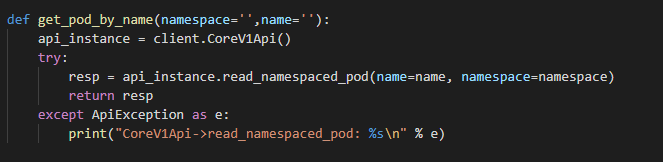
\includegraphics[width=0.90\columnwidth]{images/captures/codigo/Capture_get_pod_by_name.PNG}
	\caption{Captura del código de la función get\_pod\_by\_name().}
	\label{fig:codi01}
\end{figure}

\par En la figura \ref{fig:codi01} se muestra el código de la función  $\textbf{get\_pod\_by\_name(namespace, name)}$ la cual retorna la información de un pod a partir de su nombre, dicha función tiene como parámetros el namespace donde se encuentra el pod y su nombre. Ya que se utiliza la API del cliente de Kubernetes para Python se tiene acceso a la función \textbf{read\_namespaced\_pod(name, namespace)} la cual nos retorna el objeto con los detalles del pod. \\

\par Otra función importante de mencionar es \textbf{run\_module} la cual es básicamente el main de los tests de fallas, aquí se leen todos los parámetros recibidos por el modulo (nombre del pod a afectar, tiempo de la prueba, entre otros según el caso), se seleccionan los pod a afectar y es donde se llama a ejecutar la inyección de la falla.\\

\par También se hace gran uso de la herramienta\carlos{que parametros se han utilizado?} \textbf{stress-ng} el cual fue diseñado para ejercitar varios subsistemas físicos de una computadora, así como las diversas interfaces del kernel del sistema operativo. La herramienta tiene una amplia gama de diferentes mecanismos de estrés (conocidos como "factores de estrés") de los cuales se hizo uso y se explicaran mas adelante.\\

\subsubsection{Desarrollo de test de inyección de latencia en interfaz de red}

\begin{figure}[htpb!]
	\centering
	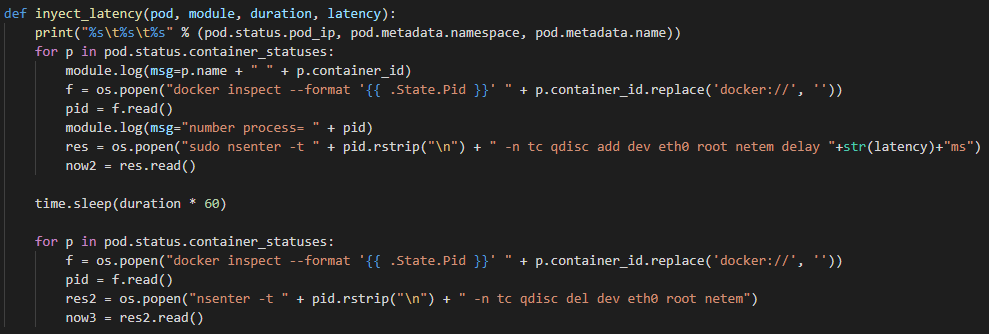
\includegraphics[width=0.95\columnwidth]{images/captures/codigo/Capture_inyect_latency.PNG}
	\caption{Captura del código de la función inyect\_latency().}
	\label{fig:codi02}
\end{figure}

\par En la figura \ref{fig:codi02} se puede observar la función \textbf{ inyect\_latency(pod, module, duration, latency)} la cual esta encargada de inyectar latencia en la interfaz de red de un pod.\\

\par La función recibe por parámetro los detalles del pod a probar, la instancia del modulo de ansible, la duración de la falla respectivamente y la cantidad en ms de latencia que el usuario quiera inyectar. \\

\par Utilizando el paquete os de Python se logra ejecutar comandos de linux en la maquina que corre el nodo y obtener las respuestas que estos devuelven. \\

\par En los detalles del pod se encuentra un atributo llamado container\_statuses el cual es una lista que tiene un tamaño equivalente al numero de contenedores que se ejecutan en el pod a afectar y en cada posición almacena la información del contenedor. Se realizaran ciclos sobre este arreglo para inyectar la latencia en cada contenedor y luego también para retirar dicho estrés.\\

\par Para inyectar la latencia en un contenedor primero se tiene que saber su ID de proceso, el cual se obtiene con el ejecutando el siguiente comando en el nodo \textbf{docker inspect --format '\{\{.State.Pid \}\}' <ID del contenedor>}, una vez tenemos el ID del proceso podemos ejecutar lo siguiente \textbf{sudo nsenter -t <ID del proceso> \ -n tc qdisc add dev eth0 root netem delay <latency>ms} a continuación una explicación por partes del comando:

\begin{itemize}
        \item nsenter -t <ID del proceso> \ -n: nsenter es una herramienta que permite ejecutar comandos en distintos namespaces de linux, con la bandera -t definimos el namespace objetivo pasándole como argumento el ID del proceso y el -n sin argumento lo que indica es que se utilice la red del proceso que se coloco como objetivo.
        \item tc: Herramienta utilizada para controlar el trafico de red en el kernel de Linux.
        \item qdisc add dev eth0 root: Con el comando qdisc podemos configurar la cola de almacenamiento de una interfaz de red, básicamente en esta sección del comando se esta agregando configuración (definida en el próximo punto) sin clase a la raíz del dispositivo eth0.
        \item netem delay <latency>ms: Esta es la configuración que es agregada a la interfaz, la que se menciono en el punto anterior, netem es un emulador de red que facilita agregar características a los paquetes que salen de una interfaz de red seleccionada, en este caso se agrega un retardo de N (latencia que pasa por parámetro el usuario) en milisegundos.\\
    \end{itemize}
    
\par Una vez todos los contenedores tenga agregada la latencia se esperan N segundos (duración de la falla la cual es agregada por el usuario vía parámetro en el modulo), por ultimo se elimina la configuración que agrega el retardo en la red de todos los contenedores.\\ 

\par Para ejecutar este modulo de inyección de fallas de latencia localmente, se configur\'o el siguiente comando:
\begin{itemize}
    \item \textbf{ansible -m include\_role \ -a `name=pystol.actions.networkstresspod' \ -e `$\{$ \\
    `pystol\_networkstresspod\_namespace': `<Namespace de los Pods>', \\
    `pystol\_networkstresspod\_pod': `<Nombre del Pod o aleatorio>', \\
    `pystol\_networkstresspod\_duration': `<Duracion de la Falla', \\
    `pystol\_networkstresspod\_amount': `<Cantidad de Pods>', \\
    `ansible\_python\_interpreter': `/usr/bin/python3', \\
    `pystol\_networkstresspod\_latency': `<Cantidad de Latencia en ms>'$\}$' \ localhost} %\ -vvvv}
\end{itemize}

\subsubsection{Desarrollo de test de inyección de sobrecarga de CPU}

\begin{figure}[htpb!]
	\centering
	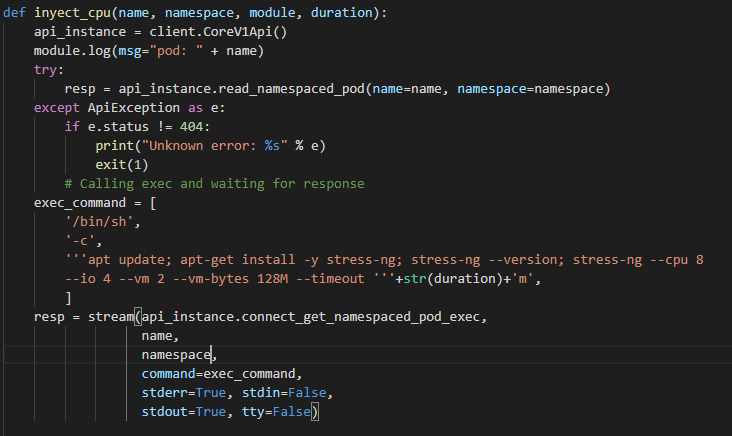
\includegraphics[width=0.95\columnwidth]{images/captures/codigo/Capture_inyect_cpu.PNG}
	\caption{Captura del código de la función inyect\_cpu().}
	\label{fig:codi03}
\end{figure}

\par En la figura \ref{fig:codi03} se puede observar la función \textbf{ inyect\_cpu(name, namespace, module, duration)} la cual esta encargada de inyectar la sobrecarga de CPU en un pod.\\
\par La función recibe por parámetro el nombre y el namespace del pod, la instancia del modulo de ansible y la duración de la falla respectivamente. \\
\par Inicialmente en esta función se crea una instancia de la API de Kubernetes para Python, luego se revisa si ciertamente existe un pod con el nombre y el namespace recibido por parámetros, a continuación se definen los comandos que se ejecutaran en el pod en los cuales se instala la herramienta stress-ng y se ejecuta la falla con el siguiente comando 
\textbf{stress-ng --cpu 8 --io 4 --vm 2 --vm-bytes 128M --timeout <duration>} a continuación una explicación de lo que significa cada bandera que se utiliza:
\carlos{esto no tiene mucho sentido, la prueba correcta sería, un pod con una aplicacion web, luego generan tráfico simulado con un criterio X, en ese momento lanzan la prueba desde ansible que satura el pod, miden como se comporta la aplicacion web, deja de responder? se crea otro pod?}
\begin{itemize}
        \item --cpu 8: Se inician 8 trabajadores que realizaran todos los trabajos de estress de CPU disponibles en stress-ng.
        \item --io 4: Se inician 4 trabajadores que realizan operaciones de entrada y salida en la cache del disco.
        \item --vm 2: Se inician 2 trabajadores que empiezan a hacer operaciones de escritura dentro de la memoria fisica asignada.        
        \item --vm-bytes 128M: Se le asignan 128 megabytes a cada trabajador de la bandera anterior.
        \item --timeout <duration>: Duración de la prueba.\\
    \end{itemize}

\par Por ultimo utilizando \textbf{stream} y \textbf{connect\_get\_namespaced\_pod\_exec} los cuales provienen de la API de Kubernetes, se logran ejecutar en el pod todos los comandos definidos previamente y recibir la respuesta.\\

\par Para ejecutar este modulo de inyección de fallas en CPU localmente, se configur\'o el siguiente comando:
\begin{itemize}
    \item \textbf{ansible -m include\_role \ -a `name=pystol.actions.cpustresspod' \ -e `$\{$ \\   
    `pystol\_cpustresspod\_namespace': `<Namespace de los Pods>',\\
    `pystol\_cpustresspod\_pod': `<Nombre del Pod o aleatorio>',\\
    `pystol\_cpustresspod\_duration': `<Duracion de la Falla>',\\
    `pystol\_cpustresspod\_amount': `<Cantidad de Pods>',\\
    `ansible\_python\_interpreter': `/usr/bin/python3'$\}$' \ localhost} % \ -vvvv}
\end{itemize}


\subsubsection{Desarrollo de test de inyección de sobrecarga de Memoria}

\begin{figure}[htpb!]
	\centering
	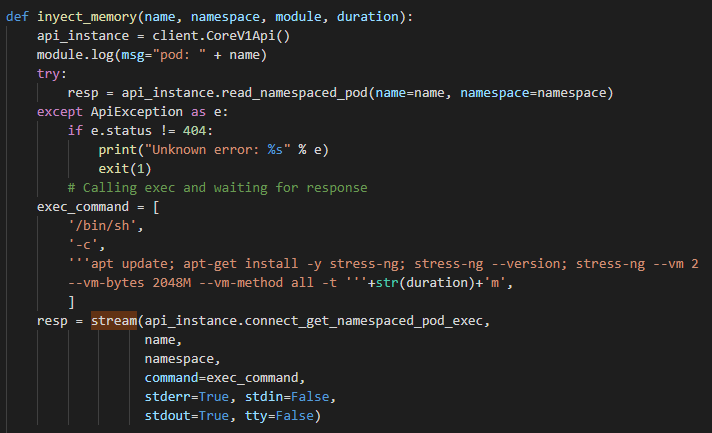
\includegraphics[width=0.95\columnwidth]{images/captures/codigo/Capture_inyect_memory.PNG}
	\caption{Captura del código de la función inyect\_memory().}
	\label{fig:codi04}
\end{figure}

\par En la figura \ref{fig:codi04} se puede observar la función \textbf{ inyect\_memory(name, namespace, module, duration)} la cual esta encargada de inyectar la sobrecarga en la memoria RAM de un pod.\\
\par La función recibe por parámetro el nombre y el namespace del pod, la instancia del modulo de ansible y la duración de la falla respectivamente. \\
\par Inicialmente en esta función se crea una instancia de la API de Kubernetes para Python, luego se revisa si ciertamente existe un pod con el nombre y el namespace recibido por parámetros, a continuación se definen los comandos que se ejecutaran en el pod en los cuales se instala la herramienta stress-ng y se ejecuta la falla con el siguiente comando
\textbf{stress-ng --vm 2 --vm-bytes 2048M --vm-method all -t <duration> } a continuación una explicación de lo que significa cada bandera que se utiliza:
\begin{itemize}
        \item --vm 2: Se inician 2 trabajadores que empiezan a hacer operaciones de escritura dentro de la memoria fisica asignada.        
        \item --vm-bytes 2048M: Se le asignan 2048 megabytes a cada trabajador de la bandera anterior.
        \item --vm-method all: Para que utilice todos los métodos disponibles en stress-ng de pruebas de memoria.
        \item -t <duration>: Duración de la prueba.\\
    \end{itemize}

\par Por ultimo utilizando \textbf{stream} y \textbf{connect\_get\_namespaced\_pod\_exec} los cuales provienen de la API de kubernetes, se logran ejecutar en el pod todos los comandos definidos previamente y recibir la respuesta.\\

\par Para ejecutar este modulo de inyección de fallas en memoria localmente, se configur\'o el siguiente comando:
\begin{itemize}
    \item \textbf{ansible -m include\_role \ -a `name=pystol.actions.memorystresspod' \ -e `$\{$ \\
    `pystol\_memorystresspod\_namespace': `<Namespace de los Pods>', \\
    `pystol\_memorystresspod\_pod': `<Nombre del Pod o aleatorio>', \\
    `pystol\_memorystresspod\_duration': `<Duracion de la Falla>', \\
    `pystol\_memorystresspod\_amount': `<Cantidad de Pods>', \\
    `ansible\_python\_interpreter': `/usr/bin/python3'$\}$' \ localhost} %\ -vvvv}
\end{itemize}



\subsubsection{Desarrollo de test de inyección de sobrecarga de Disco}

\begin{figure}[htpb!]
	\centering
	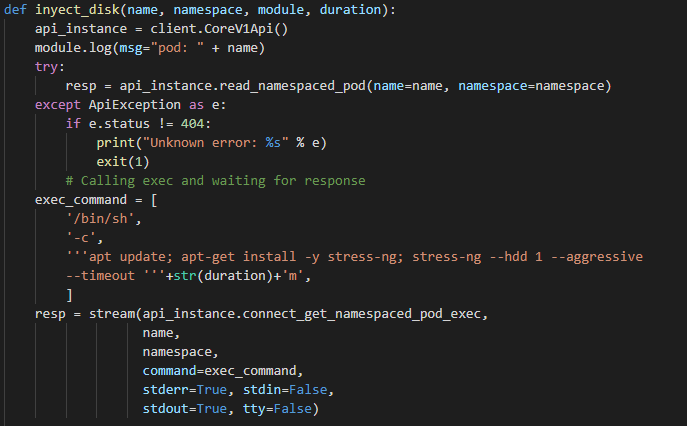
\includegraphics[width=0.95\columnwidth]{images/captures/codigo/Capture_inyect_disk.PNG}
	\caption{Captura del código de la función inyect\_disk().}
	\label{fig:codi05}
\end{figure}

\par En la figura \ref{fig:codi05} se puede observar la función \textbf{ inyect\_disk(name, namespace, module, duration)} la cual esta encargada de inyectar la sobrecarga en el disco.\\
\par La función recibe por parámetro el nombre y el namespace del pod, la instancia del modulo de ansible y la duración de la falla respectivamente. \\

\carlos{que es sobrecarga de disco?}
\par Inicialmente en esta función se crea una instancia de la API de Kubernetes para Python, luego se revisa si ciertamente existe un pod con el nombre y el namespace recibido por parámetros, a continuación se definen los comandos que se ejecutaran en el pod en los cuales se instala la herramienta stress-ng y se ejecuta la falla con el siguiente comando
\textbf{stress-ng --hdd 1 --aggressive --timeout <duration> } a continuación una explicación de lo que significa cada bandera que se utiliza:
\begin{itemize}
        \item --hdd 1: Se inicia un trabajador que escribe, lee y elimina archivos temporales en el disco.        
        \item --aggressive: Para que utilice todas las opciones disponibles en stress-ng que realicen operaciones de entrada y salida en el disco.
        \item --timeout <duration>: Duración de la prueba.\\
    \end{itemize}

\par Por ultimo utilizando \textbf{stream} y \textbf{connect\_get\_namespaced\_pod\_exec} los cuales provienen de la API de kubernetes, se logran ejecutar en el pod todos los comandos definidos previamente y recibir la respuesta.\\

\par Para ejecutar este modulo de inyección de fallas en disco localmente, se configur\'o el siguiente comando:
\begin{itemize}
    \item \textbf{ansible -m include\_role \ -a `name=pystol.actions.diskstresspod' \ -e `$\{$ \\
    `pystol\_diskstresspod\_namespace': `<Namespace de los Pods>', \\
    `pystol\_diskstresspod\_pod': `<Nombre del Pod o aleatorio>', \\
    `pystol\_diskstresspod\_duration': `<Duracion de la Falla>', \\
    `pystol\_diskstresspod\_amount': `<Cantidad de Pods>', \\
    `ansible\_python\_interpreter': `/usr/bin/python3'$\}$' \ localhost} %\ -vvvv}
\end{itemize}
\carlos{hace falta una tabla con los parametros de configuracion}

\subsection{Implementación y despliegue de herramientas del sistema}
\par Una vez teniendo las pruebas de inyección de fallas y el ambiente de estas implementado, fue necesario el despliegue de pods con características especificas para poder observar y caracterizar el comportamiento del cluster de Kubernetes con un solo nodo; también la obtención de métricas y resultados.\\
\subsubsection{Obtenci\'on de m\'etricas de Kubernetes: metrics-server}

\par Las métricas de uso de los recursos, como la CPU del pod y el uso de la memoria de este, están disponibles en Kubernetes a través de la API de métricas. Un usuario puede acceder a estas métricas directamente con un comando o un controlador en el clúster, por ejemplo el controlador encargado de escalar los pods horizontalmente. Metrics-Server es un agregador de datos de uso de recursos y es un componente a nivel de clúster que periódicamente extrae las métricas de todos los nodos de Kubernetes que ofrece Kubelet. A través de la API de métricas, puede obtener la cantidad de recursos que utiliza actualmente un nodo o un pod determinado, esta API no almacena los valores de las métricas, por lo que no es posible obtener valores de uso históricos sin el uso de herramientas de terceros \cite{WEB03}. Al consultar el servidor por linea de comandos se pueden obtener las siguientes métricas: 
\begin{itemize}
    \item \textbf{CPU:} El uso de CPU se informa como el uso promedio, en núcleos de CPU, durante un período de tiempo, este valor se obtiene tomando una tasa sobre un contador de CPU acumulativo proporcionado por el kernel (tanto en Linux como Windows) y Kubelet elige la ventana de tiempo para el cálculo del valor.
    \item \textbf{Memoria:} La memoria se informa como el \textit{working set} o ``conjunto de trabajo'', en bytes, en el instante en que se recopiló la métrica, el \textit{working set} es la cantidad de memoria en uso que no se puede liberar bajo la presión de la memoria. Sin embargo, el cálculo del conjunto de trabajo varía según el sistema operativo del host y por lo general, se produce una estimación. Incluye toda la memoria anónima (no respaldada en archivos), ya que Kubernetes no admite el swap, la métrica también incluye algo de memoria en caché (respaldada por archivos), porque el sistema operativo del host no siempre puede reclamar dichas páginas.
\end{itemize}

\par Para hacer uso del metrics-server por comandos es necesario realizar los pasos a continuación:
\begin{enumerate}
    \item Se ejecuta el siguiente comando para habilitar el servidor de metricas dentro del cluster (es necesario levantar Minikube):
    \begin{itemize}
        \item \textbf{minikube addons enable metrics-server}
    \end{itemize}
    \item Una vez habilitado metrics-server se puede consultar la ultima medicion realizada con:
    \begin{itemize}
        \item \textbf{kubectl top}
        \item \textbf{kubectl top pods} para obtener los recursos utilizados por los pods.
    \end{itemize}
\end{enumerate}

\subsubsection{Implementación y despliegue de pods: Nginx}

\par A fin de medir los efectos adversos que ocasionan estas fallas y también obtener un estado inicial estable considerable, fueron desplegados deployments con imágenes de contenedor de Nginx. Estos deployment de Nginx fueron usados para proveer un entorno de pruebas comprensible, para así obtener métricas entendibles, antes y después de la ejecución de los experimentos de inyección de fallas.\\

\par Para poder insertar fallas y medir sus resultados fueron desplegados 2 Nginx deployments (uno de control y otro pruebas) cada uno con 2 replicas. Ambos deployments poseen 2 pods activos, también se despliegan dos servicios los cuales prestan los deployments en la red local y son expuestos por un puerto asignado por Kubernetes. 

\begin{figure}[htpb!]
	\centering
	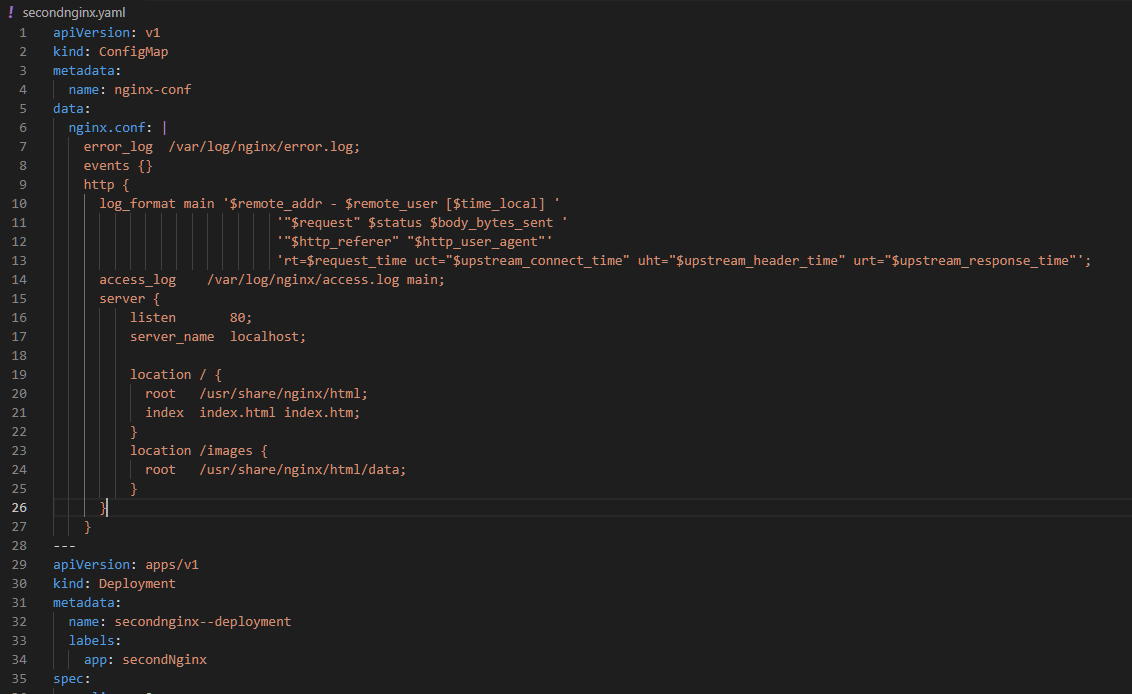
\includegraphics[width=0.95\columnwidth]{images/captures/podnginx/second01.PNG}
	\caption{Archivo de despliegue de deployment .YAML (parte\#1).}
	\label{fig:yml01}
\end{figure}

\begin{figure}[htpb!]
	\centering
	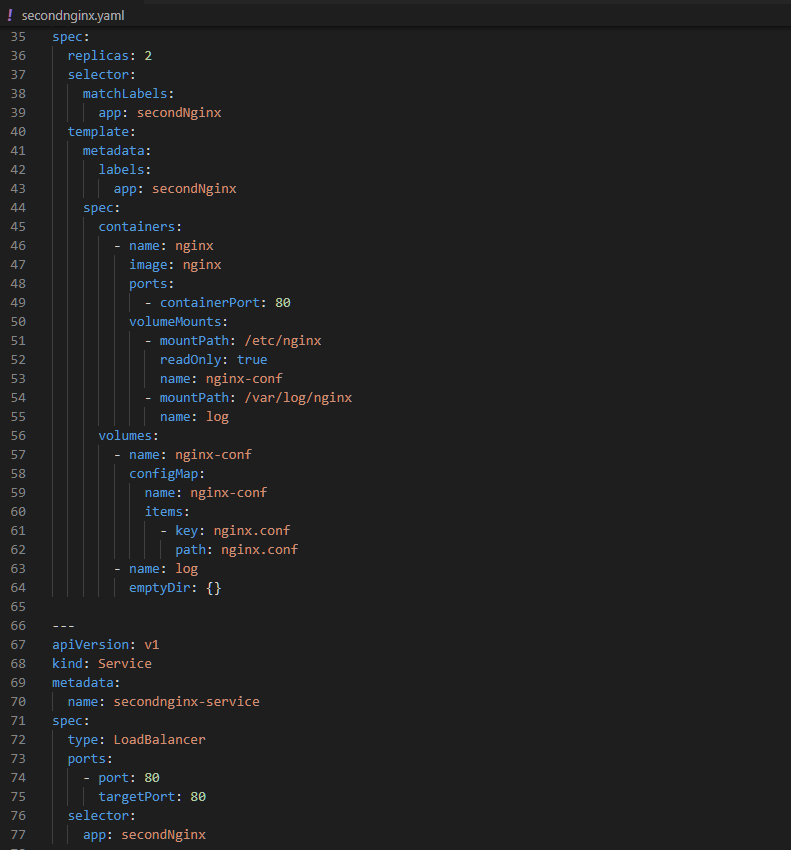
\includegraphics[width=0.95\columnwidth]{images/captures/podnginx/second02.PNG}
	\caption{Archivo de despliegue de deployment .YAML (parte\#2)}
	\label{fig:yml02}
\end{figure}

\par En las figuras \ref{fig:yml01} y \ref{fig:yml02}, se puede observar el archivo .YAML desarrollado para el despliegue de los deployments de Nginx. En dicho el archivo se puede observar características previamente mencionadas, como la creación de 2 replicas de la imagen de Nginx, también se puede ver la creación del servicio y que cada una de estas replicas posee volúmenes del tipo configMap (el cual no es compartido por ambas replicas). En este archivo se configura el uso de los logs de nginx, realizando el cambio necesario dentro del archivo nginx.conf que se encuentra en el volumen de cada pod. Se habilitan los 2 logs, el \textit{error.log} y el \textit{access.log}, el mas relevante sera el log access, ya que se revisara para obtener los tiempos de respuesta por cada solicitud que realiza un cliente al servicio de los deployment. Se le da formato a \textit{access.log} solicitando las variables requeridas para obtener la métrica deseada (el \textit{request time} o tiempo de solicitud, tiempos de respuesta o response time). Es necesario realizar el comando \textbf{kubectl apply -f <deployFile.YAML>} para que se apliquen los cambios y se desplieguen los deployments necesarios con sus respectivos pods y servicios.\\

\par El deployment de Nginx se encarga de servir una pagina simple, en la cual un usuario puede escribir un URL de una imagen para que la pagina la muestre. El documento HTML para el deployment de pruebas cuenta con un peso total de 17628379 bytes (17MB aproximadamente), ambos pods del deployment se encargan de mostrar el mismo sitio por el servicio asignado.\\

\begin{figure}[htpb!]
	\centering
	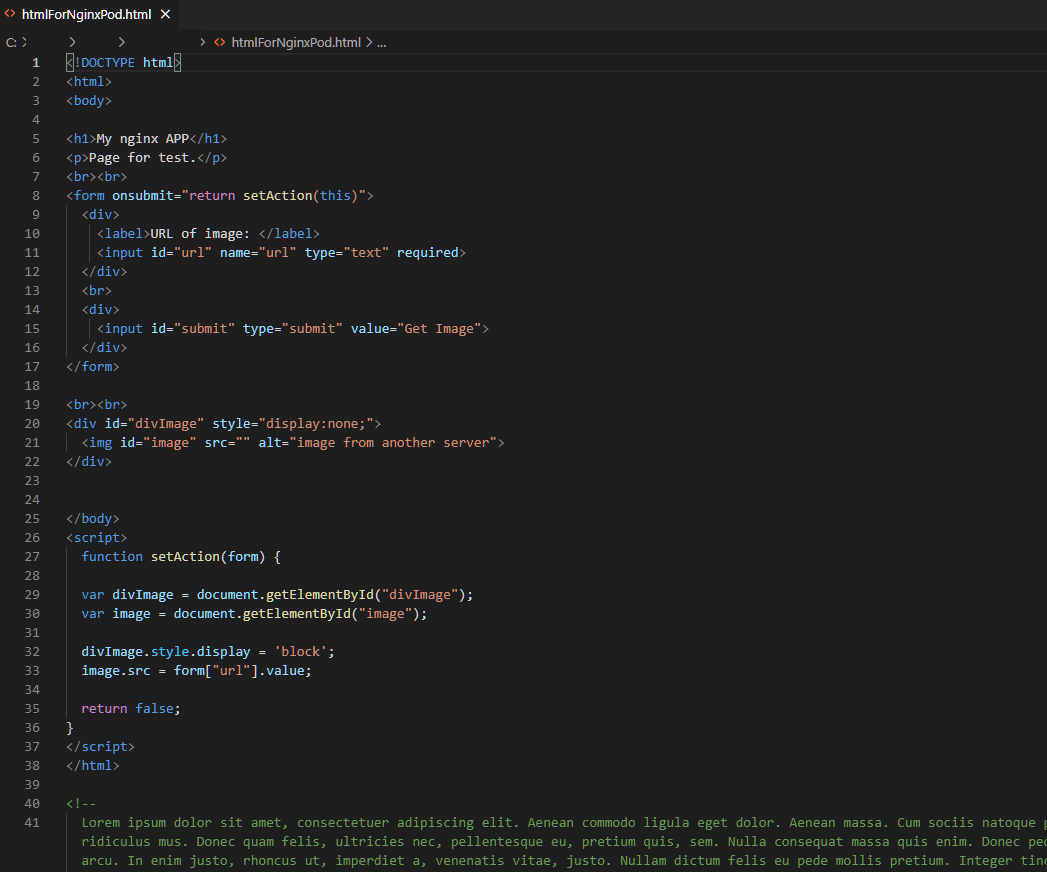
\includegraphics[width=0.95\columnwidth]{images/captures/podnginx/html01.PNG}
	\caption{Archivo Html par los deployments de Nginx.}
	\label{fig:html01}
\end{figure}

\par Se realizo la inserción de una gran cantidad de comentarios (ver Figura \ref{fig:html01}), para incrementar el peso en almacenamiento de la pagina y obtener valores significativos de tiempos de repuesta medibles, es decir, tiempo de respuesta $\textbf{rt > 0.000}$ cuando un cliente realice una solicitud. Para cambiar el index.html de cada pod se uso el comando \textbf{kubectl cp <htmlFileDrirectory>/<htmlFile> <podIdentifier>:/usr/share/nginx/html/index.html} que copia el archivo del equipo al pod. Una vez copiado se puede acceder a la p\'agina, a través de un navegador en un equipo que se encuentre en la red local, para obtener el URL del servicio se ejecuta el comando \textbf{minikube service <serviceName>}, que en este caso es secondnginx-service debido que este es el que se muestra como ejemplo en el .YAML.\\

\par Cada vez que alguien realiza una petición al servicio, dicha solicitud se ve reflejada en el access log de Nginx, el cual puede ser revisado copiando el archivo desde el pod al equipo realizando \textbf{kubectl cp <podIdentifier>:/var/log/nginx/access.log <directoryForCopy>/access.log}, luego se accede al log con uso de un editor de texto como vim o nano y se pueden observar las metricas de request\_time y response\_time.\\ 

\par Así fue implementado en su totalidad el ambiente a usar para probar el funcionamiento de los test, así como, los pods para los experimentos y poder medir métricas simples, de fácil lectura. 
%\subsubsection{Depliegue de pods: Prometheus}
%%%%%%%%%%

\subsection{Evaluaci\'on del sistema de fallas desarrollado}

\par El grupo de experimentos a continuación demostraran que las pruebas de inyección de fallas están comportándose de la manera esperada.\\ 

\par Cabe destacar que todos los experimentos de esta sección se realizaran en una maquina virtual que utiliza un disco HDD, con dos cores de CPU y 4GB de RAM.\\

\par Para medir objetivamente el desempeño del sistema se debe definir un conjunto de indicadores que nos permitan comparar los resultados obtenidos.\\

\par Como el funcionamiento del sistema de inyección de fallas depende de cuatro módulos: latencia, CPU, memoria y disco se utilizaran distintos indicadores para cada modulo los cuales se explican a continuación:
\begin{itemize}
    \item Latencia: Se utilizara el ping para su medición, se expresa en milisegundos (ms) es el tiempo que tardan en comunicarse dos puntos en la red.
    \item Memoria RAM: Se expresara su uso en mebibyte (Mi), su equivalencia en bytes es la siguiente: \[ 1\ mebibyte = 1\ Mi = 2^{20}\ bytes = 1.048.576\ bytes \]
    \item CPU: Se utilizara la unidad de Kubernetes llamada millicpu (m) en el cual se divide un núcleo de CPU en 1000 unidades.
    \item Disco: Se expresara con el porcentaje de operaciones de entrada y salida en disco.
\end{itemize} 

\carlos{todas las tablas de los resultados no tienen sentido, deben mostrar el estado del cluster en funcion del tiempo}
\carlos{RESPONDER PARA CADA PRUEBA:}

\carlos{- Objetivo}
\carlos{- Por que es interesante medir ese aspecto del desempeño del cluster, por ejemplo, por que es interesante medir la latencia}

\carlos{- Cual es la duracion de cada prueba? Donde se configura? Como se ejecuta?}
\par Se cuantific\'o un estado estable inicial, sobre los pods de un despliegue de control antes de realizar cualquier test, el cual proporciono las siguientes métricas iniciales, sobre ambos pods del deployment:
\begin{table}[ht!]
\begin{center}
\begin{tabular}{ |c|c| } 
 \hline
 \multicolumn{2}{|c|}{Estado inicial} \\
 \hline
 \hline
 Métrica & Valor(Aprox.)\\
 \hline
 CPU(millicpu) & 0 mCpu\\
 Memoria(mebibytes) & 3 Mi \\
 Uso Disco(\%) & 1.00 \% \\
 Latencia(milisegundos) & 0.055 ms\\
 %Request Time (rt) & 0.492 s\\
 \hline
\end{tabular}
\end{center}
\caption{Métricas iniciales Deployment.}
\label{tab:tabla40}
\end{table}

\par Los valores de CPU y Memoria se obtienen utilizando la herramienta del metrics-server de Minikube, siendo consultado varias veces antes de los experimentos. Para medir el Request Time o tiempo de solicitud, se accedió al servicio a través de un navegador sin almacenar cache, luego se realizaron dos solicitudes al servicio por minuto, durante 30 minutos, se reviso el access.log de ambos pod del deployment y se calculo el promedio de los tiempos de solicitud en dicho log.


\subsubsection{Probando el estrés por CPU}

\carlos{Aqui hace falta una grafica que muestre el uso del CPU en funcion del tiempo, en un estado normal}
\carlos{Aqui hace falta una grafica que muestra el uso del CPU en funcion del tiempo mientras se ejecuta el fault injection}

\par Se probara la inyección de falla estudiando el uso inicial del CPU en millicpu (antes del estrés) de un pod de Nginx que tiene dos cores de CPU, luego se estresara al agregarle la sobrecarga de CPU y por ultimo se observara el estado (mientras sucede la falla) para compararlo con el inicial y así demostrar que esta funcionando dicha falla.\\

\par Para obtener el indicador en millicpu en cada estado, se utilizara el comando \\ \verb|kubctl top pods| desde la maquina virtual que tiene alojado a Kubernetes, dicho comando básicamente permite ver el consumo de recursos de los pods.\\

\begin{table}[ht!]
\begin{center}
\begin{tabular}{ |c|c| } 
 \hline
 \multicolumn{2}{|c|}{Resultado} \\
 \hline
 \hline
 Estado & CPU(millicpu)\\
 \hline
 Inicial & 0\\
 Falla & 1658\\
 \hline
\end{tabular}
\end{center}
\caption{Tabla comparativa del uso del CPU en los estados del experimento de estrés por CPU.}
\label{tab:tabla41}
\end{table}


\par Con el resultado se puede observar el aumento sustancial del uso del CPU, el pod afectado durante el estrés esta usando aproximadamente el 80\% del CPU, por lo cual esta funcionando correctamente la inyección de fallas.\\

\subsubsection{Probando el estrés por latencia}

\carlos{Aqui hace falta una grafica que muestre la latencia en funcion del tiempo, en un estado normal}
\carlos{Aqui hace falta una grafica que muestra la latencia en funcion del tiempo mientras se ejecuta el fault injection}

\par Se probara la inyección de falla por latencia estudiando el ping inicial (antes del estrés) de un pod de Nginx, luego se estresara al agregarle un ping de 500ms y por ultimo se observara el estado (mientras sucede la falla) para compararlo con el inicial y así demostrar que esta funcionando dicha falla.\\

\par Para obtener el indicador del ping en cada estado, se utilizara el comando \\ \verb|ping -c 4 <IP del pod afectado>| desde la maquina virtual que tiene alojado a Kubernetes, dicho comando básicamente enviara cuatro solicitudes de ICMP hacia la IP del pod afectado y luego mostrara las respuesta de cada solicitud en la cual se podrá observar el tiempo que tarda cada paquete en llegar a su destino y regresar (ping en ms).\\
\begin{table}[ht!]
\begin{center}
\begin{tabular}{ |c|c| } 
 \hline
 \multicolumn{2}{|c|}{Resultado} \\
 \hline
 \hline
 Estado & Ping(promedio)\\
 \hline
 Inicial & 0.055ms\\
 Falla & 500.5ms\\
 \hline
\end{tabular}
\end{center}
\caption{Tabla comparativa del ping en los estados del experimento de estrés por latencia.}
\label{tab:tabla42}
\end{table}

\vspace{\baselineskip}
\par Con el resultado se puede observar el aumento de 500ms en el ping en el estado de falla, por lo cual esta funcionando correctamente el estrés por latencia.\\

\subsubsection{Probando el estrés por memoria RAM}

\carlos{Aqui hace falta una grafica que muestre el uso de la memoria principal en funcion del tiempo, en un estado normal}
\carlos{Aqui hace falta una grafica que muestra el uso de la ram en funcion del tiempo mientras se ejecuta el fault injection}

\par Se probara la inyección de falla estudiando el uso inicial de memoria RAM en mebibyte (antes del estrés) de un pod de Nginx, luego se estresara al agregarle la sobrecarga de memoria RAM y por ultimo se observara el estado (mientras sucede la falla) para compararlo con el inicial y así demostrar que esta funcionando dicha falla.\\

\par Para obtener el indicador en mebibyte en cada estado, se utilizara el comando \\ \verb|kubctl top pods| desde la maquina virtual que tiene alojado a Kubernetes, dicho comando básicamente permite ver el consumo de recursos de los pods.\\
\begin{table}[ht!]
\begin{center}
\begin{tabular}{ |c|c| } 
 \hline
 \multicolumn{2}{|c|}{Resultado} \\
 \hline
 \hline
 Estado & Memoria(mebibytes)\\
 \hline
 Inicial & 2\\
 Falla & 2059\\
 \hline
\end{tabular}
\end{center}
\caption{Tabla comparativa del porcentaje de uso de la memoria RAM en los estados del experimento de estrés por memoria.}
\label{tab:tabla43}
\end{table}

\vspace{\baselineskip}
\par Con el resultado se puede observar el aumento sustancial del uso de la memoria RAM, por lo cual esta funcionando correctamente la inyección de fallas.\\

\subsubsection{Probando el estrés por disco}

\carlos{Aqui hace falta una grafica que muestre el uso del disco  funcion del tiempo, en un estado normal}
\carlos{Aqui hace falta una grafica que muestra el uso del disco en funcion del tiempo mientras se ejecuta el fault injection}

\par Se probara la inyección de falla estudiando el porcentaje de escritura y lectura inicial del disco (antes del estrés) de un pod de Nginx, luego se estresara al agregarle muchas operaciones al disco y por ultimo se observara el estado (mientras sucede la falla) para compararlo con el inicial y así demostrar que esta funcionando dicha falla.\\

\par Para obtener el indicador en porcentaje en cada estado, se utilizara el comando \\ \verb+iostat -dxy 2 1 | awk '/sda/{print $NF}'+ desde el pod que se utilizara para la prueba, dicho comando básicamente nos mostrara el porcentaje de escritura y lectura del disco sda.\\

%-dxy es estadisticas ampliadas (-x) por dispositivos (-d) omitiendo el primer reporte desde el arranque del sistema (y), 2 seg de espera 1 repeticion y mandamos a imprimir la ultima columna de la fila de sda.  

\begin{table}[ht!]
\begin{center}
\begin{tabular}{ |c|c| } 
 \hline
 \multicolumn{2}{|c|}{Resultado} \\
 \hline
 \hline
 Estado & E/S Disco(porcentaje)\\
 \hline
 Inicial & 1.00\\
 Falla & 96.80\\
 \hline
\end{tabular}
\end{center}
\caption{Tabla comparativa del porcentaje de E/S del disco en los estados del experimento de estrés por disco.}
\label{tab:tabla44}
\end{table}

\par Con el resultado se puede observar el aumento sustancial de las operaciones de escritura y lectura en el disco, por lo cual esta funcionando correctamente la inyección de fallas.\\



\section{Evaluacion del sistema de fallas en un entorno de Kubernetes}

\carlos{Cada experimento debe llevar una grafica en funcion del tiempo (duracion del experimento) donde se pueda apreciar el comportamiento habitual y el fallo que estan inyectando}.

\carlos{que criterio estan utilizando para generar ese "trafico", sobrecarga, o latencia?}

\par Una vez desarrollado el sistema de inyección de fallas, se realizaron varios experimentos para estudiar el comportamiento de Kubernetes al sufrir fallas. En esta sección se explican los experimentos realizados y se ilustran los resultados obtenidos.\\


\par Se medira objetivamente el desempeño del sistema con el tiempo de solicitud el cual es la duracion total empleada por Nginx para procesar una solicitud y se expresa en segundos. Dicha metrica permitira comparar los resultados obtenidos utilizando distintos casos de prueba.\\


% \par Esta sección se dividirá en dos partes, la primera en la que se estudiara el correcto funcionamiento de las inyecciones de fallas y la segunda parte en la que se observara y analizará el comportamiento de Kubernetes al sufrir fallas en sus pods.\\


% \subsection{Experimentos del comportamiento de Kubernetes}

% \par En el grupo de experimentos a continuación se busca estudiar el comportamiento de Kubernetes ante fallas.\\ 

\par Se preparo un pod de Nginx que servirá un documento HTML que ocupa 16.8 MB de espacio en disco, a su vez Nginx esta configurado para almacenar los logs de acceso en el cual tendremos la métrica de tiempo de solicitud, dicha variable se estará utilizando para representar el tiempo en segundos que tardo procesar la solicitud y así estudiar el rendimiento durante una falla.\\

\par Se creo un servicio de Kubernetes que servirá dos replicas del pod anteriormente descrito con el fin de comprobar si Kubernetes pudo realizar correctamente el balanceo de carga.\\

\par Cabe destacar que todos los experimentos de esta sección se realizaran en una maquina virtual que utiliza un disco HDD, con dos cores de CPU y 4GB de RAM.\\

\par Se determino una metrica inicial, sobre los pods de un despliegue, previo a realizar cualquier test o caso, el cual proporciono el siguiente valor promedio del tiempo de solicitud (rt), sobre ambos pods del deployment:
\begin{table}[ht!]
\begin{center}
\begin{tabular}{ |c|c| } 
 \hline
 \multicolumn{2}{|c|}{Estado inicial} \\
 \hline
 \hline
 Tiempo de Solicitud & Valor Promedio Inicial\\
 \hline
 Request Time (rt) & 0.492 s\\
 \hline
\end{tabular}
\end{center}
\caption{Tiempo de Solicitud inicial.}
\label{tab:tabla406}
\end{table}

\subsubsection{Caso \#1: Falla de CPU en una replica}

\carlos{como han medido el rendimiento? en funcion del tiempo de respuesta de la aplicacion? que aplicacion está funcionando?}

\par Se inyecto la falla de CPU en una replica durante 5 minutos, a continuación el resultado en el rendimiento del servicio.\\

\begin{table}[ht!]
\begin{center}
\begin{tabular}{ |c|c| } 
 \hline
 \multicolumn{2}{|c|}{Resultado} \\
 \hline
 \hline
 Estado & Tiempo de solicitud(segundos)\\
 \hline
 Inicial & 0.492\\
 Falla & 1.300\\
 \hline
\end{tabular}
\end{center}
\caption{Tabla comparativa del tiempo de solicitud en los estados del caso \#1.}
\label{tab:tabla45}
\end{table}


\par Se pudo observar que el pod afectado utilizo entre 1500 y 1700 de mCPU durante la falla. También se observ\'o que, Kubernetes logro hacer un balanceo de carga ya que la replica que respondió las solicitudes no fue la que se encontraba afectada con la falla del CPU, sin embargo, se pudo notar un leve aumento en el tiempo de solicitud porque el CPU del nodo en general se vio comprometido con la falla.\\

\subsubsection{Caso \#2: Falla de CPU en dos replicas}

\par Se inyecto la falla de CPU en las dos replicas durante 15 minutos, a continuación el resultado en el rendimiento del servicio.\\

\begin{table}[ht!]
\begin{center}
\begin{tabular}{ |c|c| } 
 \hline
 \multicolumn{2}{|c|}{Resultado} \\
 \hline
 \hline
 Estado & Tiempo de solicitud(segundos)\\
 \hline
 Inicial & 0.492\\
 Falla & 10.037\\
 \hline
\end{tabular}
\end{center}
\caption{Tabla comparativa del tiempo de solicitud en los estados del caso \#2.}
\label{tab:tabla46}
\end{table}

\par Se pudo observar un aumento considerable del tiempo de solicitud, Kubernetes repartió el total del CPU disponible entre las 2 replicas, cada una con un uso entre 800 y 900 de mCPU (entre 1600 y 1700 total entre ambas) sin embargo esto no resuelve la falla simplemente realizo un balanceo del recurso en el nodo.\\

\subsubsection{Caso \#3: Falla de disco en una replica}

\par Se inyecto la falla de disco en una replica durante 5 minutos, a continuación el resultado en el rendimiento del servicio.\\

\begin{table}[ht!]
\begin{center}
\begin{tabular}{ |c|c| } 
 \hline
 \multicolumn{2}{|c|}{Resultado} \\
 \hline
 \hline
 Estado & Tiempo de solicitud(segundos)\\
 \hline
 Inicial & 0.492\\
 Falla & 1.900\\
 \hline
\end{tabular}
\end{center}
\caption{Tabla comparativa del tiempo de solicitud en los estados del caso \#3.}
\label{tab:tabla47}
\end{table}

\par Se pudo notar que Kubernetes respondió las solicitudes con ambas replicas (la que poseía la falla y la que no, es decir, no hubo balanceo en esta falla), en ambas replicas se pudo notar un leve aumento en el tiempo de solicitud ya que ambas replicas comparten el mismo disco del nodo, aunque cada una posee su propio volumen y solo era afectado el uso de disco en el pod con falla.\\

\subsubsection{Caso \#4: Falla de disco en dos replicas}

\par Se inyecto la falla de disco en las dos replicas durante 15 minutos, a continuación el resultado en el rendimiento del servicio.\\

\begin{table}[ht!]
\begin{center}
\begin{tabular}{ |c|c| } 
 \hline
 \multicolumn{2}{|c|}{Resultado} \\
 \hline
 \hline
 Estado & Tiempo de solicitud(segundos)\\
 \hline
 Inicial & 0.492\\
 Falla & 3.700\\
 \hline
\end{tabular}
\end{center}
\caption{Tabla comparativa del tiempo de solicitud en los estados del caso \#4.}
\label{tab:tabla48}
\end{table}

\par Se pudo observar un leve aumento (a diferencia de las otras pruebas sobre ambos pods) del tiempo de solicitud, ambas replicas dieron respuesta a las solicitudes, Kubernetes no se pudo recuperar de esta falla durante el tiempo que duro el experimento.\\

\subsubsection{Caso \#5: Falla por latencia en una replica}

\par Se inyecto la falla por latencia en una replica durante 5 minutos, a continuación el resultado en el rendimiento del servicio.\\

\begin{table}[ht!]
\begin{center}
\begin{tabular}{ |c|c| } 
 \hline
 \multicolumn{2}{|c|}{Resultado} \\
 \hline
 \hline
 Estado & Tiempo de solicitud(segundos)\\
 \hline
 Inicial & 0.492\\
 Falla & 0.820\\
 \hline
\end{tabular}
\end{center}
\caption{Tabla comparativa del tiempo de solicitud en los estados del caso \#5.}
\label{tab:tabla49}
\end{table}

\par Se pudo observar que Kubernetes logro hacer un balanceo de carga ya que la replica que respondió las solicitudes no fue la que se encontraba con latencia inyectada, dicha replica sin fallas no se vio afectada por el estrés que se le realizo a su replica hermana, no hubo incremento en el tiempo de respuesta del servicio debido al balanceo.\\

\subsubsection{Caso \#6: Falla por latencia en las dos replicas}

\par Se inyecto la falla por latencia en dos replicas durante 15 minutos, a continuación el resultado en el rendimiento del servicio.\\

\begin{table}[ht!]
\begin{center}
\begin{tabular}{ |c|c| } 
 \hline
 \multicolumn{2}{|c|}{Resultado} \\
 \hline
 \hline
 Estado & Tiempo de solicitud(segundos)\\
 \hline
 Inicial & 0.492\\
 Falla & 6.820\\
 \hline
\end{tabular}
\end{center}
\caption{Tabla comparativa del tiempo de solicitud en los estados del caso \#6.}
\label{tab:tabla50}
\end{table}

\par Se pudo observar un aumento considerable del tiempo de solicitud, ambas replicas se encontraban afectadas con 500ms de latencia, Kubernetes no se pudo recuperar de esta falla durante el tiempo que duro el experimento.\\

\subsubsection{Caso \#7: Falla de memoria RAM en una replica}

\par Se inyecto la falla de memoria RAM en una replica durante 5 minutos, a continuación el resultado en el rendimiento del servicio.\\

\begin{table}[ht!]
\begin{center}
\begin{tabular}{ |c|c| } 
 \hline
 \multicolumn{2}{|c|}{Resultado} \\
 \hline
 \hline
 Estado & Tiempo de solicitud(segundos)\\
 \hline
 Inicial & 0.492\\
 Falla & 1.592\\
 \hline
\end{tabular}
\end{center}
\caption{Tabla comparativa del tiempo de solicitud en los estados del caso \#7.}
\label{tab:tabla51}
\end{table}

\par Se pudo observar al pod afectado con un mayo de 2100 MiB de memoria. También que Kubernetes logro hacer un balanceo de carga ya que la replica que respondió las solicitudes no fue la que se encontraba con la falla, sin embargo, se pudo notar un leve aumento en el tiempo de solicitud del servicio, porque la memoria del nodo en general se vio comprometido con la falla.//

\subsubsection{Caso \#8: Falla de memoria RAM en dos replicas}

\par Se inyecto la falla de memoria RAM en las dos replicas durante 15 minutos, a continuación el resultado en el rendimiento del servicio.\\

\begin{table}[ht!]
\begin{center}
\begin{tabular}{ |c|c| } 
 \hline
 \multicolumn{2}{|c|}{Resultado} \\
 \hline
 \hline
 Estado & Tiempo de solicitud(segundos)\\
 \hline
 Inicial & 0.492\\
 Falla & 4.164\\
 \hline
\end{tabular}
\end{center}
\caption{Tabla comparativa del tiempo de solicitud en los estados del caso \#8.}
\label{tab:tabla52}
\end{table}

\par Se pudo observar un aumento considerable del tiempo de solicitud, ambas replicas poseían entre 1700 y 2000 MiB de memoria en uso cada una, no los 2048 mínimos de la falla (el total de uso entre ambos no supero los 4096 MiB total del nodo), Kubernetes no se pudo recuperar de esta falla durante el tiempo que duro el experimento y se observo notificaciones de procesos encargados de inyectar fallas detro de los pods, siendo eliminados por el sistema operativo del nodo, debido al evento OOM (\textit{Out of Memory}).\\

		%\input{chaptern}
		\chapter{Conclusiones y Trabajos futuros}

%%%%%%%%%%%%%%%%%%%%%%%%%%%%%%%%%%%%%%%%%%%%%%%%
\section{Conclusiones}

\par Una vez desarrolladas las 4 fases divididas en capítulos que conforman la presente investigación, se puede concluir lo siguiente:\\
\par Es necesario que las organizaciones que prestan servicios en la nube, sometan a prueba sus sistemas desplegados basados en entornos de computo híbrido, antes, durante y después de su desarrollo, debido al auge que \'estos poseen en la actualidad, mas aun hacen uso de recursos de infraestructura como son los de hardware tales como CPU, memoria y disco, entre otros. Igualmente, señalar la importancia de los recursos de red en este tipo de despliegues, para proveer una buena calidad en la prestación de estos servicios. \\

\par Por lo anteriormente expuesto, en el capitulo 2 de este trabajo se realiz\'o la recopilación y el estudio de las bases teóricas contentivas de las diversas definiciones y conceptos existentes de las herramientas, tecnologías y disciplinas utilizadas por las organizaciones antes referidas. Asimismo, se indicaron las características de la herramientas esenciales para el desarrollo de este estudio como son Kubernetes y Ansible comparándolas con su competencia. Por otra parte, se describieron las disciplinas que permiten comprobar la fiabilidad de sistemas basados en las tecnologías previamente mencionadas, que se encuentren en sus fases desarrollo y producción, como es la inyección de fallas y su forma mas actual que es la ingeniería del caos (Chaos Engineering). Todo este conocimiento fue relevante y pertinente, con el fin de lograr la solución el problema objeto de esta investigación. \\

\par En lo concerniente a las metodologías de desarrollo, se expusieron las metodologías pesadas y las ligeras, tomando en consideración las ventajas de unas sobre otras, para realizar la selección mas adecuada. De modo que, se seleccion\'o la metodología ligera Kanban con todas sus modificaciones necesarias para su uso en esta trabajo, puesto que permite la definición de las tareas ejecutadas para la implementación del proyecto. Es importante destacar, que en el tablero Kanban se definió las actividades necesarias para realizar la implementación del entorno de pruebas, diseño de test de inyección, desarrollo de test de inyección basados en colecciones y roles de Ansible. Además, se planificaron los experimentos que evaluaron el funcionamiento de las pruebas y observaron el comportamiento del cluster de Kubernetes de un solo nodo, por lo cual la  aplicación de esta metodología que se caracteriza por el trabajo en equipo, result\'o exitosa por no ser rígida. \\ 

\par En cuanto a las herramientas seleccionadas para poder implementar un ambiente de pruebas, se evidenci\'o que Kubernetes es la herramienta óptima para desplegar los microservicios debido a su amplia aceptacion en la actualidad, así como también, por el fácil acceso a la documentación y el gran soporte que posee. En relación con Ansible, su uso se basa en los conocimientos previos que se dominan de la herramienta, y proporciona estupendas características para su uso. De ahí que, fue posible la implementación de la arquitectura propuesta en el capitulo 4, tanto en AWS como en un equipo local, con la configuración mínima planteada empleando herramientas de software libre.\\ 

\par De igual modo, se estableció el entorno donde se realizaron las pruebas de inyección de fallas, documentándose cada uno de los pasos seguidos. Así que, se diseñaron las pruebas que van a afectar los recursos de CPU, memoria, disco y red sobre los objetos seleccionados (Pods de Kubernetes), siguiendo los artefactos creados como guía para el desarrollo de los tests, que fueron implementados con el lenguaje de programación Python y se definen documentos en .YAML. Asimismo, se manejaron paquetes de software accesibles en el ambiente de Linux, como lo es stress-ng, con mecanismos denominados ``estresadores'' diseñados para estresar los recursos al forzar al hardware y software de un equipo, lo cual permitió aumentar el consumo de memoria, CPU y uso de disco exitosamente en los pods. Posteriormente, se utiliz\'o el control de tr\'afico tc que provee el sistema Linux para limitar el uso de la interfaz y simular problemas en los recursos de red, que al ser medidos con un simple ping brindan resultados, tales como el incremento de la latencia en los pods.\\

\par En la fase experimental de este trabajo, se presenta el desarrollo, evaluacion y aplicacion de un sistema de inyeccion de fallas dirigido a Kubernetes. En los resultados obtenidos se evidenció que la herramienta Kubernetes posee mecanismos de resistencia a las mismas, tales como el balanceo de carga en los servicios con réplicas, donde Kubernetes daba prioridad de respuesta del servicio desde el pod que no se encontraba en un estado ``enfermo''. De igual forma, aplica balanceo en los recursos, evitando que algún pod acapare el uso del CPU o la memoria si se excede de los límites, y en caso de eventos como presión en la memoria RAM (si algún pod supera el límite configurado) o del disco en el nodo, puede llegar a reiniciar o cancelar la ejecución de pods. También se constató, que existen capacidades como configurar limites de recursos dentro de los pods, que permiten evitar casos de abuso de recurso dentro del nodo por los mismos pods.\\

\par Para concluir, se diseñaron e implementaron los tests para simular fallos en entornos de cómputo híbrido (en especifico Kubernetes de un solo nodo). A su vez, que se logró desplegar un entorno de pruebas y se caracterizó la respuesta de éste a dicha simulación, consiguiendo cumplir con los objetivos propuestos en la sección \ref{sec:41} en casi toda su totalidad, solo difiriendo en la falta de recopilación de datos en casos de pérdida de paquetes debido a que no se notó ninguna así como tampoco, se consiguió la interrupción del servicio, pero si se alcanzó a deteriorar la calidad de la prestación del mismo.


%%%%%%%%%%%%%%%%%%%%%%%%%%%%%%%%%%%%%%%%%%%%%%%%
\section{Trabajos futuros}
\par Se proponen los siguientes trabajos futuros:

\begin{itemize}
\item Creación de mas parámetros en las fallas para que el usuario pueda personalizar mas el estrés que quiera aplicar.
\item Implementar una interfaz de usuario que permita controlar las fallas con un mayor nivel de usabilidad y simplicidad.
\item Diseñar un sistema de reportes, esto permitirá al usuario conocer mas a fondo lo que sucedió antes, durante y después de que fue inyectada la falla.
\end{itemize}


	\backmatter
		\bibliographystyle{IEEEtran}
		\renewcommand\bibname{Referencias}
		%\bibliographystyle{plain}     %You may prefer \bibliographystyle{alpha}
		%\bibliographystyle{alpha}
		%\bibliographystyle{babalpha}
		\bibliography{books}
		%\nocite{*}
		%\chapter{Anexos}

%%%%%%%%%%%%%%%%%%%%%%%%%%%%%%%%%%%%%%%%%%%%%%%%
Documentos, tablas, cronogramas, c\'alculos, planos etc. que dificulten la lectura del informe y que han sido citados en \'este. Agregar \# c\'odigo fuente	%opcional
\end{document}